\documentclass[12pt,          % font size: 11pt or 12pt
               phd,           % degree:    ms or phd
               onehalfspacing % spacing: onehalfspacing or doublespacing
               ]{ncsuthesis}

%%----------------------------------------------------------------------------%%
%%------------------------------ Import Packages -----------------------------%%
%%----------------------------------------------------------------------------%%

\usepackage{booktabs}  % professionally typeset tables
\usepackage{amsmath}
\usepackage{textcomp}  % better copyright sign, among other things
\usepackage{xcolor}
\usepackage{lipsum}    % filler text
\usepackage{longtable}
%\usepackage{subfig}    % composite figures
%\usepackage{natbib}    % ability to use citet,citep
\usepackage[backend=biber, natbib=true, style=apa]{biblatex}
\addbibresource{StudentName-thesis.bib}
%\usepackage{fancyhdr}  % creates headers
%\pagestyle{fancy}


%%---------------------------------------------------------------------------%%
%%  Bibliography 
%% or use BibTeX
%\bibliography{StudentName-thesis}
%% \bibliographystyle{apalike}


% Citations should be of the form ``author year''  not ``author, year''
% \bibpunct{(}{)}{;}{a}{}{,} % changes apalike bst into AMS format
 
%%----------------------------------------------------------------------------%%
%%---------------------------- Formatting Options ----------------------------%%
%%----------------------------------------------------------------------------%%
%%

%% -------------------------------------------------------------------------- %%
%% Disposition format -- any titles, headings, section titles
%%  These formatting commands affect all headings, titles, headings,
%%  so sizing commands should not be used here.
%%  Formatting options to consider are
%%     +  \sffamily - sans serif fonts.  Dispositions are often typeset in
%%                    sans serif, so this is a good option. 
%%     +  \rmfamily - serif fonts
%%     +  \bfseries - bold face
%\dispositionformat{\sffamily\bfseries}   % bold and sans serif
\dispositionformat{\bfseries}            % bold and serif

%% -------------------------------------------------------------------------- %%
%% Formatting for centered headings - Abstract, Dedication, etc. headings
%%  This is where one might put a sizing command.
%%  \MakeUppercase can be used to typeset all headings in uppercase.
\headingformat{\large\MakeUppercase}   % All letters uppercase
%\headingformat{\large}                % Not all uppercase
%\headingformat{\Large\scshape}        % Small Caps, used with serif fonts.

%% Typographers recommend using a normal inter-word space after
%% sentences. TeX's default is to add an wider space, but \frenchspacing
%% gives a normal spacing. Comment out the following line if you prefer wider spaces between sentences.
\frenchspacing

%% -------------------------------------------------------------------------- %%
%%  Optional packages
%%    A number of compatible packages to improve the look and feel of
%%    your document are available in the file optional.tex 
%%    (For example, hyperlinks, fancy chapter headings, and fonts)
%% To use these options, uncomment the next line and see optional.tex
%%  Optional Packages to consider.   These packages are compatible with
%%    ncsuthesis.  

%% -------------------------------------------------------------------------- %%
%% Fancy chapter headings
%%  available options: Sonny, Lenny, Glenn, Conny, Rejne, Bjarne
%\usepackage[Sonny]{fncychap}
\usepackage[Rejne]{fncychap}

%%----------------------------------------------------------------------------%%
%% Hyperref package creates PDF metadata and hyperlinks in Table of Contents
%%  and citations.  Based on feedback from the NCSU thesis editor, 
%%  the links are not visually distinct from normal text (i.e. no change
%%  in color or extra boxes).
\usepackage[
  pdfauthor={Change author in optional.tex},
  pdftitle={Change title in optional.tex},
  pdfcreator={pdftex},
  pdfsubject={NC State ETD Dissertation},
  pdfkeywords={change key words in optional.tex},
  colorlinks=true,
  linkcolor=black,
  citecolor=black,
  filecolor=black,
  urlcolor=black,
]{hyperref}


%% -------------------------------------------------------------------------- %%
%% Microtype - If you use pdfTeX to compile your thesis, you can use
%%              the microtype package to access advanced typographic
%%              features.  By default, using the microtype package enables
%%              character protrusion (placing glyphs a hair past the right 
%%              margin to make a visually straighter edge)
%%              and font expansion (adjusting font width slightly to get 
%%              more favorable justification).
%%              Using microtype should decrease the number of lines
%%              ending in hyphens.
\usepackage{microtype}


%%----------------------------------------------------------------------------%%
%% Fonts 

%% ETD guidelines don't specify the font.  You can enable the fonts
%%  by uncommenting the appropriate lines.  Using the default Computer 
%%  Modern fonts is *not* required.  A few common choices are below.
%%  See http://www.tug.dk/FontCatalogue/ for more options.

%% Serif Fonts -------------------------------------------------
%%  The four serif fonts listed here (Utopia, Palatino, Kerkis,
%%  and Times) all have math support.


%% Utopia
\usepackage[T1]{fontenc}
\usepackage[adobe-utopia]{mathdesign}

%% Palatino
%\usepackage[T1]{fontenc}
%\usepackage[sc]{mathpazo}
%\linespread{1.05}

%% Kerkis
%\usepackage[T1]{fontenc}
%\usepackage{kmath,kerkis}

%% Times
%\usepackage[T1]{fontenc}
%\usepackage{mathptmx}


%% Sans serif fonts -------------------------

%\usepackage[scaled]{helvet}  % Helvetica
%\usepackage[scaled]{berasans} % Bera Sans



%solve bug from fancyhdr in optional
%http://nw360.blogspot.com/2006/11/latex-headheight-is-too-small.html
%\setlength{\headheight}{26.94345pt} % corrected error in Overleaf
%\fancyhead[L]{\vspace{1mm}} % only puts chapter title in headers

%%----------------------------------------------------------------------------%%
%%---------------------------- Content Options -------------------------------%%
%%----------------------------------------------------------------------------%%
%% Size of committee: 3, 4, 5, or 6 -- this number includes the chair
\committeesize{5}

%% Members of committee
%%  Each of the following member commands takes an optional argument
%%   to specify their role on the committee.
%%  For co-chairs, use the commands:
%%      \cochairI{Doug Dodd}
%%      \cochairII{Chris Cox}
%%
\chair{Rubén Rellán Álvarez}
\memberI{Rubén Rellán Álvarez}
\memberII{James Holland}
\memberIII{Jung-Ying Tzeng}   % unnecessary if committeesize=3
\memberIV{Rafael Guerrero}    % unnecessary if committeesize=3, 4

%% Student writing thesis, \student{First Middle}{Last}
\student{Fausto Villafrade}{Rodríguez Zapata} % a full middle name

%% Degree program e.g. Marine, Earth, and Atmospheric Science
\program{Genetics}

%%!!!!!! To Change Year !!!!!!%%
% If year of graduation is not same as current year (common for December graduates
% thanks to the Grad Schools odd graduation rules) go into ncsuthesis.cls and change 
% \the\year in the line:
% \newcommand{\ncsu@year}{\the\year}
% to the year of graduation. E.g.:
% \newcommand{\ncsu@year}{2020}

%% Thesis Title
%%  Keep in mind, according to ETD guidelines:
%%    +  Capitalize first letter of important words.
%%    +  Use inverted pyramid shape if title spans more than one line.
%%
%%  Note: To break the title onto multiple lines, use \break instead of \\.
%\thesistitle{A North Carolina State University Sample \LaTeX{} Thesis \break 
%with a Title So Long it Needs a Line Break}
\thesistitle{Genomic Insights Into the Role of Phospholipid Metabolism and Soil Phosphorus Availability in Maize Adaptation to Highlands}

%% Degree year. Necessary if your degree year doesn't equal the current year.
%\degreeyear{1995}

%% While your here make sure to change the PDF characteristics in optional.tex!!!

%%----------------------------------------------------------------------------%%
%%---------------------------- Personal Macros -------------------------------%%
%%----------------------------------------------------------------------------%%

%% A central location to add your favorite macros.

%% A few examples to get you started.
\newcommand{\uv}[1]{\ensuremath{\mathbf{\hat{#1}}}}
\newcommand{\bo}{\ensuremath{\mathbf{\Omega}}}
\newcommand{\eref}[1]{Eq.~\ref{#1}}
\newcommand{\fref}[1]{Fig.~\ref{#1}}
\newcommand{\tref}[1]{Table~\ref{#1}}

%% Add commonly used words
\newcommand{\mex}{\textit{mexicana}\xspace}
\newcommand{\hpc}{\textit{HPC1}\xspace}
\newcommand{\invfour}{\textit{Inv4m}\xspace}
\newcommand{\parv}{\textit{parviglumis}\xspace}

%% code inline frormatiing 
\newcommand{\code}{\texttt}

%%---------------------------------------------------------------------------%%
\begin{document}

%%---------------------------------------------------------------------------%%
\frontmatter

%% ------------------------------ Abstract ---------------------------------- %%
\begin{abstract}

Maize had no major artificial phosphorus input during its evolution in domestication and breeding until modern industrial agriculture.
Currently yield  relies on a steady but limited supply of mined phosphate fertilizer.
Even so,  traditional farmers in Mexico still successfully grow varieties with no addition of industrial fertilizer. Understanding the nature of the genetic variation underlying this adaptation can contribute to the production of phosphorus efficient crops that could lower costs and water pollution from leached fertilizers.
In this study I establish genome environment associations (GEA) between soil phosphorus availability, from interpolated soil profile maps, and the genetic diversity of a collection of ~2000 open-pollinated varieties in Mexico. Here I find evidence of association between a chromosomal inversion, inv4m, and multiple soil phosphorus parameters, specially, water soluble phosphorus and phosphorus retention.
Although this inversion is presumed to be adaptive to high elevation in Mexico no current measurements of fitness exists where inv4m has been experimentally isolated from background genetic variation. To test whether inv4m is adaptive, I used a segregating HIF population for inv4m, derived from a cross of the temperate inbred B73 and  the Mexican Andosol variety MICH21, grown in the field under high and low phosphorus treatments.
In addition to this I built both an expression and a phospholipid profile from a developmental series of leaves. Complementing the GEA approach I made a QTL search for seed phosphorus content using ionomics. or this I used 8 families of BC2S3 RILs, derived from parents traditionally cultivated in Mexican Andosols and the tropical line CML530.
Results show that inv4m accelerates flowering independent of phosphorus treatments at our test field in Pennsylvania. This the first direct experimental evidence of the adaptive contribution of  inv4m, however the adaptation is rather global  in character, with respect to soil phosphorus availability.
As inv4m does not show the pattern of Gene X Environment interaction expected in the case of local adaptation. Currently I am doing the gene expression analysis o test the efect of inv4m on gene expression pre-reproductive leaves. In our multiparental population I was able to detect 2 QTLs for seed phosphorus content in chromosomes 7 and 8, furthter analyses are required to characterize possible candidates. 
\end{abstract}


%% ---------------------------- Copyright page ------------------------------ %%
%% Comment the next line if you don't want the copyright page included.
\makecopyrightpage

%% -------------------------------- Title page ------------------------------ %%
\maketitlepage

%% -------------------------------- Dedication ------------------------------ %%
%\begin{dedication}
% \centering To my parents.
%\end{dedication}

%% -------------------------------- Biography ------------------------------- %%
\begin{biography}
The author was born in a small town \ldots
\end{biography}

%% ----------------------------- Acknowledgements --------------------------- %%
%\begin{acknowledgements}
%Thanks to family, advisor, committee, office friends, etc. ...
%\end{acknowledgements}


\thesistableofcontents

\thesislistoftables

\thesislistoffigures


%%---------------------------------------------------------------------------%%
\mainmatter

% Chapters can remove or add
% \setcounter{chapter}{-1}
\chapter{Introduction}
\label{chap-zero}

% Please add the following required packages to your document preamble:
% \usepackage{booktabs}
% \usepackage{graphicx}
% Please add the following required packages to your document preamble:
% \usepackage{booktabs}
% \usepackage{graphicx}
\begin{table}[]
\caption{\textbf{Key Locations Showing Diverse Phosphorus conditions}}
\label{tab:locations}
\resizebox{\textwidth}{!}{%
\begin{tabular}{@{}lllllllll@{}}
\multicolumn{1}{c}{\textbf{Site}} &
  \multicolumn{1}{c}{\textbf{Relevant Germplasm}} &
  \multicolumn{1}{c}{\textbf{\begin{tabular}[c]{@{}c@{}}Soil\\ pH\end{tabular}}} &
  \multicolumn{3}{c}{\textbf{Soil Phosphorus}} &
  \multicolumn{2}{c}{\textbf{Soil Classification}} &
  \multicolumn{1}{c}{\textbf{Section}} \\ \cmidrule(lr){4-8}
\multicolumn{1}{c}{} &
  \multicolumn{1}{c}{} &
  \multicolumn{1}{c}{} &
  \multicolumn{1}{c}{\textbf{\begin{tabular}[c]{@{}c@{}}ppm\\ (mg/kg)\end{tabular}}} &
  \multicolumn{1}{c}{\textbf{\begin{tabular}[c]{@{}c@{}}Method\\ (notes)\end{tabular}}} &
  \multicolumn{1}{c}{\textbf{Retention}} &
  \multicolumn{1}{c}{\textbf{\begin{tabular}[c]{@{}c@{}}WRB\\ Group\end{tabular}}} &
  \multicolumn{1}{c}{\textbf{\begin{tabular}[c]{@{}c@{}}USDA\\ Order\end{tabular}}} &
  \multicolumn{1}{c}{} \\ \midrule
\begin{tabular}[c]{@{}l@{}}Puerto Vallarta\\ (Bahía de Banderas)\\ Nayarit, México\\ 20°47'2" N 105°14'31" W\end{tabular} &
  \begin{tabular}[c]{@{}l@{}}Grown: \\ PT (MEXI210, AN26)\\ B73\\ PTxB73 RILs\\ AIR (SMS)\end{tabular} &
  7.3 &
  28 &
  Olsen &
  Low &
  Phaeozem &
  Mollisol &
  \begin{tabular}[c]{@{}l@{}}HPC1\\ Kernel Ionomics\end{tabular} \\
 &
   &
   &
   &
   &
   &
   &
   &
   \\
\begin{tabular}[c]{@{}l@{}}Metepec\\ (Toluca)\\ Estado de México, México\\ 19°13'41" N 99°33'1" W\end{tabular} &
  \begin{tabular}[c]{@{}l@{}}Grown:\\ PT (MEXI210, AN26)\\ B73\end{tabular} &
  5.9 &
  91 &
  Bray &
  Low &
  Phaeozem &
  Mollisol &
  HPC1 \\
 &
   &
   &
   &
   &
   &
   &
   &
   \\
\begin{tabular}[c]{@{}l@{}}Ames\\ (Boone)\\ Iowa, USA\\ 42°1'20" N 93°46'36" W\end{tabular} &
  \begin{tabular}[c]{@{}l@{}}Bred: \\ B73\end{tabular} &
  6.2-6.8 &
  13-18 &
  \begin{tabular}[c]{@{}l@{}}Bray\\ (Optimum)\end{tabular} &
  Low &
  Phaeozem &
  Mollisol &
  HPC1 \\
 &
   &
   &
   &
   &
   &
   &
   &
   \\
\begin{tabular}[c]{@{}l@{}}Santa Mónica\\ (Ocuilán)\\ Estado de México, México\\ 18°58'10" N 99°23'57" W\\ 2445 masl\end{tabular} &
  \begin{tabular}[c]{@{}l@{}}Collected:\\ PT (MEXI210, AN26)\end{tabular} &
  6.3 &
  30 &
  Bray &
  Very High &
  Andosol &
  Andisol &
  \begin{tabular}[c]{@{}l@{}}HPC1\\ Kernel ionomics\end{tabular} \\
 &
   &
   &
   &
   &
   &
   &
   &
   \\
\begin{tabular}[c]{@{}l@{}}Rock Springs\\ Pennsylvania, USA\\ 40°42'36" N 77°57'0" W\end{tabular} &
  \begin{tabular}[c]{@{}l@{}}Grown:\\ B73 \\ PTxB73 RILs\\ B73xMICH21 NILs\end{tabular} &
  6.8 &
  \begin{tabular}[c]{@{}l@{}}5 \\ 35\end{tabular} &
  \begin{tabular}[c]{@{}l@{}}Mehlich 3\\ (Low P)\\ (High P)\end{tabular} &
  Low &
  Luvisol &
  Alfisol &
  Inv4m \\
 &
   &
   &
   &
   &
   &
   &
   &
   \\
\begin{tabular}[c]{@{}l@{}}Zacapu\\ Michoacán, México\\ 19°48'0" N 101°47'0" W\\ 2038 masl\end{tabular} &
  \begin{tabular}[c]{@{}l@{}}Collected:\\ MICH21\end{tabular} &
  6.4 &
  54 &
  Bray &
  Very High &
  Andosol &
  Inceptisol &
  Inv4m \\
 &
   &
   &
   &
   &
   &
   &
   &
   \\
\begin{tabular}[c]{@{}l@{}}Santander de Quilichao\\ Cauca, Colombia\\ 3°4'18" N 76°29'54" W\end{tabular} &
  \begin{tabular}[c]{@{}l@{}}Bred:\\ CML530\end{tabular} &
  4.5 &
  5-8 &
  Bray &
  High &
  Acrisol &
  Ultisol &
  Kernel Ionomics \\
 &
   &
   &
   &
   &
   &
   &
   &
   \\
\begin{tabular}[c]{@{}l@{}}Carimagua\\ Meta, Colombia\\ 4°34'25" N 71°20'10" W\end{tabular} &
  \begin{tabular}[c]{@{}l@{}}Grown:\\ CML530\end{tabular} &
  5.2 &
  10 &
  Bray &
  Very high &
  Ferralsol &
  Oxisol &
  Kernel Ionomics \\
 &
   &
   &
   &
   &
   &
   &
   &
   \\
\begin{tabular}[c]{@{}l@{}}Clayton\\ North Carolina, USA\\ 35°40'9" N 78°29'38" W\end{tabular} &
  \begin{tabular}[c]{@{}l@{}}Grown:\\ CML530\\ AIR (TMVB)\end{tabular} &
  6.2 &
  205-622 &
  \begin{tabular}[c]{@{}l@{}}Mehlich 3\\ (Range)\end{tabular} &
  Very high &
  Nitisol &
  Ultisol &
  Kernel Ionomics
\end{tabular}%
}
\end{table}

%% Following sections are examples... not required
%--
\section{Definitions}
\label{sec:def}
%--

Define common terms used throughout the dissertation... 

E.g. African Easterly Waves (AEWs) are waves in the atmosphere over Africa of wavelength ...

%--
\section{Motivations}
\label{sec:mot}
%--

Motivations for studying topic

%--
\section{Background}
\label{sec:back}
%--

Background literature on topic


\begin{figure}[htp]
\centering
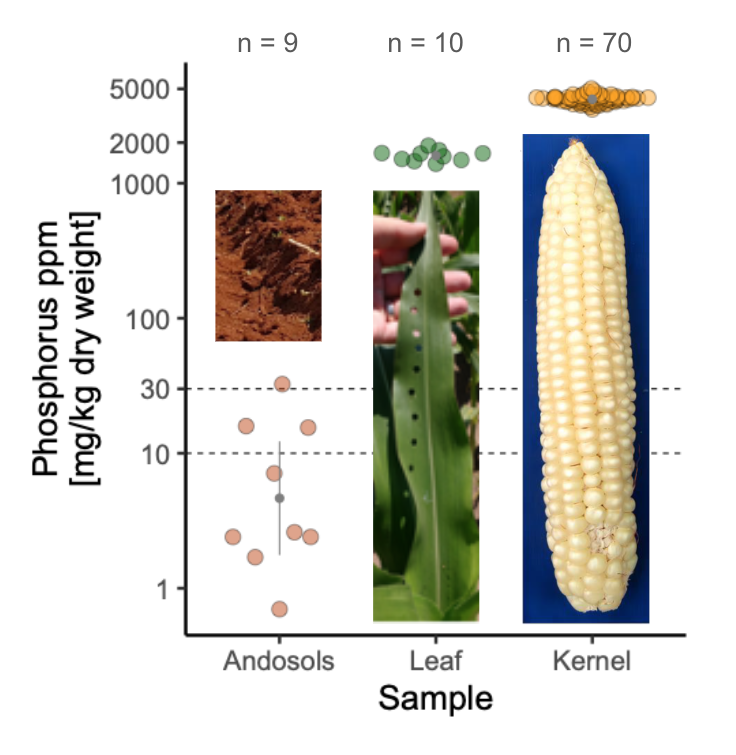
\includegraphics[width=0.5\linewidth]{Chapter-0/figs/P_soil_tissue.png}
\caption[Available phosphorus in soil and total phosphorus in maize tissues]
{\textit{\textbf{Available phosphorus in soil and total phosphorus in maize tissues.}}}
\label{fig::P_soil_tissue}
\end{figure}

%----------
\section{Open Questions and Theories}
\label{sec:que}
%----------

In this section I will present the open questions on the problem I am investigating. 

% \subsection{}
% \label{sec:QTaew-conv}

Background on theories

In summary we will attempt to address the following questions with regard to ...:
\begin{enumerate}
\item Question 1?
\item Question 2?
\item Question 3?
\end{enumerate}

\chapter{A Highland Teosinte Introgression Modulates Phosphatidylcholine Levels and is Associated with Maize Flowering Time}
\label{chap-one}

\newrefsection

\section{Disclaimer}

\section{Abstract}

%%%%%%%%%%%%%%%%%%%%%%%%%%%%%%%%%%%%%%%%%%%%%%%%%%%%%%%%%%%%%%%%%%%%%%%5%
\section{Background}
%%%%%%%%%%%%%%%%%%%%%%%%%%%%%%%%%%%%%%%%%%%%%%%%%%%%%%%%%%%%%%%%%%%%%%%5%

%How do organisms adapt to high elevations
Elevation gradients are associated with changes in environmental factors that impose substantial physiological constraints on an organism. 
Adaptation to highland environments is achieved via the selection of genetic variants that improve their ability to withstand lower oxygen availability \citep{Yi2010-se, Bigham2010-is}, increased ultraviolet (UV) radiation \citep{Yang2017-gs} and lower temperatures \citep{Cicconardi2020-gs}.
In particular, cold temperatures reduce thermal time accumulation, measured in growing degree days (GDDs), \citep{Gilmore1958-dx} and select for accelerated development and maturity as a compensatory mechanism \citep{Hatfield2015-od}.
%Maize domestication and expansion
Following domestication from teosinte \parv (\textit{Zea mays} ssp. \parv) \citep{Matsuoka2002-bg} in the lowland, subtropical environment of the Balsas River basin (Guerrero, M\'exico), cultivated maize (\textit{Zea mays} ssp. \textit{mays}) expanded throughout M\'exico and reached the highland valleys of central M\'exico around 6,500 years ago \citep{Piperno2001-ea}.

%Contribution of mexicana to highland maize adaptation.
In M\'exico, highland adaptation of maize was aided by substantial adaptive introgression from a second teosinte subspecies, teosinte \mex (\textit{Zea mays} ssp. \mex), that had already adapted to the highlands of M\'exico thousands of years after its divergence from teosinte \parv \citep{Hufford2013-gs, Gonzalez-Segovia2019-jy}. 
Adaptation to low temperature and soils with low phosphorus content in highland environments drove \mex genetic divergence from the lowland \parv \citep{AguirreLiguori2019-fl}.
Phenotypically, the most evident signs of \mex introgression into maize are the high levels of stem pigmentation and pubescence \citep{Lauter2004-eq} that are thought to protect against high UV radiation and low temperatures. 
The ability to withstand low temperatures and efficiently photosynthesize during the early stages of seedling development are key factors in maize highland adaptation \citep{Hardacre1980-tq}.
Indeed, recent transcriptome deep sequencing (RNA-seq) analysis showed that the inversion \textit{Inv4m}, introgressed from \mex, strongly affects the expression of genes involved in chloroplast physiology and photosynthesis \citep{Crow2020-gene}.  
Given the slow accumulation of GDDs in typical highland environments, selection has favored shorter generation  times in highland adapted maize \citep{Gates2019-xu}.
By the time maize reached the Mexican highlands, its range had already expanded far to the South, including the colonization of highland environments in the  Andes \citep{Athens2016-ep, Grobman2012-pm}. 
Andean maize adaptation occurred largely independently of \mex introgression \citep{Takuno2015-uj, Wang2020-mp}, and there is no known wild teosinte relative in South America. 
These multiple events of maize adaptation to highland environments make maize a good system to study the evolutionary and physiological mechanisms of convergent adaptation \citep{Takuno2015-uj, Wang2020-mp}.

%Photoperiod adaptation
In comparison to its southward expansion, the northward migration of maize into the modern-day United States, where summer daylengths are longer, occurred at a much slower pace \citep{Da_Fonseca2015-zh, Swarts2017-ge} due to delayed flowering of photoperiod-sensitive tropical maize lines \citep{Hung2012-ms}.
A host of evidence suggests that maize cultivation in northern latitudes was enabled by the selection of allelic variants that led to a reduction in photoperiod sensitivity to allow flowering under longer photoperiods \citep{Liang2018-af, Guo2018-on, Coles2010-db, Huang2018-ga, Yang2013-lg, Salvi2007-ku, Hung2012-ms}.
Some of the early flowering alleles that conferred an adaptive advantage in highland environments are the result of \mex introgressions into highland maize \citep{Guo2018-on}.
Maize first entered into the US via the Mexican highlands \citep{Da_Fonseca2015-zh}, and these early flowering alleles show further evidence of selection in northern latitudes \citep{Guo2018-on}, consistent with a likely role for \mex introgression(s) in maize adaptation to shorter daylength. 
When introduced into Northern Europe, photoperiod-insensitive maize from the Northern US and Canada thrived as it was already pre-adapted to northern latitudes and lower temperatures \citep{Brandenburg2017-ii}.
The genetic, physiological, and phenotypic basis of these adaptations, however, is quite limited.

Plant phospholipids, as well as other glycerolipids such as sulfolipids, galactolipids, and non-polar lipids such as triacylglycerols, are involved in plant responses to low temperatures.
Phospholipid levels are increased in plants exposed to low temperatures \citep{Degenkolbe2012-wf} and levels of unsaturated fatty acids in glycerolipids are reduced \citep{Welti2002-uk, Lynch1987-ln}, which may help maintain the fluidity of cell membranes.
Under stressful conditions, the proportions of differently shaped lipids are modulated to maintain membrane flexibility while preventing membrane leakage. 
For instance, phosphatidylcholines (PCs) are rectangular polar lipids that are well suited for the formation of bilayer membranes because the size of their glycerol backbone, choline headgroup and fatty acid tails are similar.
By contrast, lyso-phosphatidylcholine (LPC) is a triangular PC with a single acyl group that cannot form a bilayer because its headgroup is much larger than its fatty acid \citep{Jouhet2013-fv}.
LPCs do allow for some membrane movement, but high LPC concentrations act as a detergent \citep{Henriksen2010-cm} and can facilitate cell leakage and damage at low temperatures, effects that would be prevented by higher PC levels.
In cold-adapted maize temperate lines and \textit{Tripsacum} species (a distant maize relative), genes involved in  phospholipid biosynthesis show accelerated rates of protein sequence evolution, further supporting an important role for phospholipid metabolism across several species during cold adaptation \citep{Yan2019-tx}. 
Finally, multiple phospholipids can bind to Arabidopsis (\textit{Arabidopsis thaliana}) FLOWERING LOCUS T (FT) and accelerate flowering.
Recent work has shown that phosphatidylglycerol binds and sequesters FT in companion cells in low temperatures, while higher temperatures release it to the shoot apical meristem \citep{Susila2021-dz}.
There, it interacts with certain species of PC, the most abundant phospholipid in plant cells \citep{Gu2017-nd},  through an unknown mechanism \citep{Nakamura2014-qf}. 
Consistent with this observation, glycerolipid levels in maize have predictive power for flowering time \citep{Riedelsheimer2013-bd}. 

Here, we identified an adaptive teosinte \mex introgression that alters highland maize phospholipid metabolism and leads to early flowering.
Using genome scans and linkage mapping, we identified \textit{High PhosphatidylCholine1} (\hpc), a gene encoding a phospholipase A1, as a driver of high PC levels in highland maize. 
Data from thousands of genotyped landrace test-crosses grown in common garden experiments at different elevations in M\'exico showed a strong genotype-by-environment effect at the \hpc locus, where the highland allele leads to higher fitness in the highlands and reduced fitness at lower elevations.
Furthermore, we determined that the highland \hpc allele, which was introgressed from teosinte \mex, was carried northward and is now present in maize cultivars grown in the Northern US and European Flint lines.
These results suggest that the \hpc highland allele has a beneficial effect in cold, high-latitude environments, where early flowering is advantageous


%%%%%%%%%%%%%%%%%%%%%%%%%%%%%%%%%%%%%%%%%%%%%%%%%%%%%%%%%%%%%%%%%%%%%%%5%
\section{Methods}
%%%%%%%%%%%%%%%%%%%%%%%%%%%%%%%%%%%%%%%%%%%%%%%%%%%%%%%%%%%%%%%%%%%%%%%5%

\subsection{Plant Materials}
The diversity panels and mapping populations used in this manuscript for population genetics measures of selection, QTL mapping and G x E analysis have been described previously by \citep{Wang2020-mp}, \citep{Gates2019-xu}, \citep{Romero_Navarro2017-cn}, \citep{Janzen2021-lz} and \citep{Perez-Limon2022-lg}. 

\subsection{Genome Scan for Local Adaptation}
In order to conduct genome scans for signatures of adaptation we used the \textit{pcadapt} \citep{Luu2017-ws} package.
\textit{pcadapt} identifies adaptive loci by measuring how strongly loci are contributing to patterns of differentiation between major axes of genetic variation.
Under simple models \textit{pcadapt} captures major patterns of $F_{ST}$  but is conducted in a way that does not require population delimitation \citep{duforet2014genome}.
As the genome scan comparison requires a focal SNP to be compared to the first K principal components of the genotype data, it can be biased by large regions of low recombination that drive the major axes of variation in the principal components.
Thus, when SNPs from these low recombination regions are compared against principal components driven by linked loci spurious signals may arise.
To prevent this bias from occurring, we used custom scripts to calculate the principal component step separately based upon all the chromosomes except for the chromosome of the focal SNPs being tested.
The genotype data we used for this analysis was GBS data from roughly 2,000 landraces of Mexican origin collected by CIMMYT (www.cimmyt.org) as part of the SeeDs of discovery initiative (https://www.cimmyt.org/projects/seeds-of-discovery-seed/).
From this, we calculated the strength of association between each SNP and the first five principal components (excluding the chromosome of the focal SNP) using the communality statistic as implemented in \textit{pcadapt} version 3.0.4.


\subsection{Glycerolipid pathways selection}
We compiled a list of genes pertinent to glycerolipid metabolism starting with a search of all genes belonging to the \textit{Zea mays} 'Glycerophospholipid metabolism' and 'Glycerolipid metabolism' KEGG pathways \citep{kanehisa2019} (map identifiers: zma00564 and zma00561). 
With the NCBI Entrez gene identifiers in KEGG we retrieved the AGPv4 transcript identifiers used in Corncyc 8.0 \citep{portwood2019, walsh2016} from an id cross reference \href{https://www.maizegdb.org/search/gene/download_gene_xrefs.php?relative=v4}{file} found in MaizeGDB   \citep{portwood2019}.
This resulted in a list of 300 genes comprising 51 Corncyc pathways. 
Then we discarded Corncyc pathways  tangentially connected to the KEGG glycerolipid metabolism list (sharing just one enzyme with the initial KEGG list) or that we judged to belong to different biological processes (e.g 'long chain fatty acid synthesis','anthocyanin biosynthesis'). 
Finally, we added manually the 'phosphatidylcholine biosynthesis V' pathway that was missing. 
The list of 30 selected Corncyc pathways included genes outside the initial KEGG search results and raised the number of genes to 557. 
In addition to these, 37 genes were found to have an enzymatic activity related to phospholipid metabolism but not placed into any particular pathway, i.e orphan enzymes, consisting mostly of alcohol dehydrogenases. 
Sixteen additional genes found in KEGG were not annotated at all in Corncyc probably due to differences between AGPv4 and RefSeq pseudogene annotation of the maize genome. 
The list of all possible candidates coming either from KEGG or Corncyc that were orphan enzymes or were unannotated in Corncyc amounted to 597 genes (Sup. File 2). 
This process is documented in the \verb|0_get_glycerolipid_genes.R| script of the \verb|pgplipid| R package accompanying this paper \citep{fausto_rodriguez_zapata_2020_4323410}.

\subsection{Population Branch Excess Analysis}
Population Branch Excess quantifies changes in allele frequencies in focal populations relative to two independent “outgroup” populations.
We used \textit{Zea mays spp. parviglumis} as one of the outgroup populations for all four highland groups.  
The other outgroup was  Mexican lowlands  in the case of Southwestern US , Mexican highlands and Guatemalan highlands; and South American lowlands in the case of the Andes population. 
We used calculated PBE SNP values for the four populations (described in detail in \citep{Wang2020-mp}) and we tested for selection outliers SNPs in the 594 phosphoglycerolipid-related candidate genes and the 30 Corncyc pathways (556 genes).
We first defined PBE outlier SNPs as the top 5\% of the PBE score distribution; this fraction corresponds to approximately 50000 out of ~1 million genotyped SNPs in each population. 
Following \citep{Wang2020-mp}, we defined a gene as a PBE outlier if it contained an outlier SNP within the coding sequence or 10 kb upstream/downstream. 
Then we tested for over-representation of genes selected in particular subsets of populations using Fisher's exact test with the 32,283 protein-coding genes from the maize genome as background. 
For each pathway, we first selected all SNPs within coding regions and 10 kb upstream and downstream of genes in the pathway and we calculated the mean pathway PBE score. 
We then constructed a null distribution by drawing 10,000 samples without replacement of $n$ SNPs from those found within 10 kb upstream and downstream of all protein-coding genes and we obtained the mean PBE for this null distribution. 
With the set of PBE outliers for glycerolipid metabolism in the four populations, we tested for evidence of physiological or pleiotropic constraint using the $C_\chi^2$ statistic \citep{yeaman2018}. 

\subsection{QTL analysis of phospholipid levels}
We analyzed glycerophospholipid QTLs in a mapping population of 57 RILs (BC1S5) from the cross B73 x PT.
These RILs were grown in a highland site in Metepec, Edo de M\'exico at 2,600 masl during the summer of 2016 and in Puerto Vallarta, Jalisco at 50 masl during the winter of 2016/17. 
We analyzed the samples using UHPLC-QTOF, as above, and 67 leaf lipid species were identified.
For QTL analysis we calculated the mean across all fields of individual lipid mass signal. 
We also used as phenotypes the sum total of the following lipid classes: diacylglycerols, triacylglycerols, PCs and  LPCs.  
Furthermore,  we also included the log base 10 transformed ratios of LPCs/PCs and the ratios of their individual species. 
We did a simple single marker analysis  with ``scanone`` using Haley-Knott  regression, and assessed the QTL significance with 1,000 permutations.

\subsection{CRISPR-Cas9 editing of \hpc and analysis of the effect of \textit{hpc1\textsuperscript{CR}} mutant on flowering time}
CRISPR/Cas9 was used to create a \hpc mutant through Agrobacterium \textit{Agrobacterium tumefaciens}-mediated transformation of background line B104 \citep{Wu2020-nq, Char2017-uk}. 
RNA guides (gRNAs) were designed as described in \citep{Brazelton2015-co} for the B73 reference genome v4. 
The B104 and B73 sequence for \hpc were identical. 
The gRNA cassette was cloned into pGW-Cas9 using Gateway cloning. 
Two plants from the T\textsubscript{0} transgenic events were identified through genomic PCR amplification and Sanger sequencing and were self-pollinated. 
In the next generation, several plants were allowed to self.
Plants were genotyped using forward primer CAGTTCTCATCCCATGCACG and reverse primer CCTGATGAGAGCTGAGGTCC.


\subsection{Haplotype network analysis of \hpc in Mexican maize landraces and teosintes}
We extracted SNP genotypes for \hpc from the TIL teosinte accessions in the HapMap 3 imputed data \citep{Bukowski2017-ng} and the 3700 Mexican landraces in the SeeD dataset. 
With the set of 1060 accessions that were homozygous at all sites in this genomic region we calculated a haplotype network depicting the minimal spanning tree for haplotypes covering 90\% of the input accessions with the R package \code{pegas} \citep{paradis2010}, and haplotype frequencies for three elevation classes in the landraces (0--1,000; 1,000--2,000 and >3,000 masl).
\subsection{Clustering analysis of \hpc in maize inbred lines and teosintes}
Using v3 of the B73 genome, \hpc SNPs were obtained from PT (this paper), the 282 diversity panel \citep{Flint-Garcia2005-hb}, teosinte inbred lines and the German inbred lines from HapMap 3 \citep{Bukowski2017-ng}. 
The selection was made to have a good representation of tropical, temperate and European inbred lines together with teosintes and PT lines.
SNPs were aligned using Geneious2020.0.5 and a neighbor-joining cluster analysis was generated. 
To facilitate visualization and interpretation of the tree we condensed cluster branches from lines with identical haplotypes and from similar geographic locations. 
The full tree is available as Sup. file 9. 
\subsection{Expression analysis of candidate genes and association with flowering traits in the 282 diversity panel}
We used gene expression RNA-seq data obtained from the 282 diversity panel at different developmental stages \citep{Kremling2018-gn} and BLUP values of several flowering and photoperiod sensitivity traits \citep{Hung2012-ms} to study the correlation of \hpc expression values with flowering time traits.  

\clearpage

\section{Results}

%%%%%%%%%%%%%%%%%%%%%%%%%%%%%%%%%%%%%%%%%%%%%%%%%%%%%%%%%%%%%%%%%%%%%%%%%%%%%%%%%%%%%%%
\subsection{Genes involved in PC/LPC conversion show strong highland selection signals} 
%%%%%%%%%%%%%%%%%%%%%%%%%%%%%%%%%%%%%%%%%%%%%%%%%%%%%%%%%%%%%%%%%%%%%%%%%%%%%%%%%%%%%%%
We selected a set of 597 maize glycerolipid genes from their functional annotations (see Materials and Methods) to identify selection signals using the Population Branch Excess (PBE) \citep{Pool2017-oa} statistic across four highland populations: Southwestern US (SWUS), Mexican highlands (MH), Guatemalan highlands (GH) and Andes (AN) (\cref{Fig1}E) \citep{Wang2020-mp}. 
We identified a significant excess of genes that are targets of selection in more than two populations ($ p< 3 \times 10^{-5}$, \ref{Fig1}F).
The most over-represented intersection of selected glycerolipid genes was between the SWUS, MH and GH populations ($p = 1  \times 10 ^{-15} $, \cref{Fig1}F), suggesting that genes were specifically selected in these three populations relative to the AN population and/or that there was closer kinship among SWUS, MH, and GH populations than the AN population and thus weaker statistical independence.
From all annotated glycerolipid genes, 23 were consistently PBE outliers across all four highland populations ($p =<1  \times  ^{-10}$, \cref{Fig1}F).
We then assigned a PBE value to each of the 30 glycerolipid metabolism pathways (using a 10 kb window around each constituent gene)  and compared their average PBE value with a genome-wide random sampling distribution of PBE values within genic regions. 
From these, we established that 'phospholipid remodeling' and 'PC acyl editing' exhibit significantly higher PBE values in all four populations, indicating a possible role for phospholipid remodeling in maize highland adaptation
(\cref{Fig1}G). 

\begin{figure}[ht]
\centering
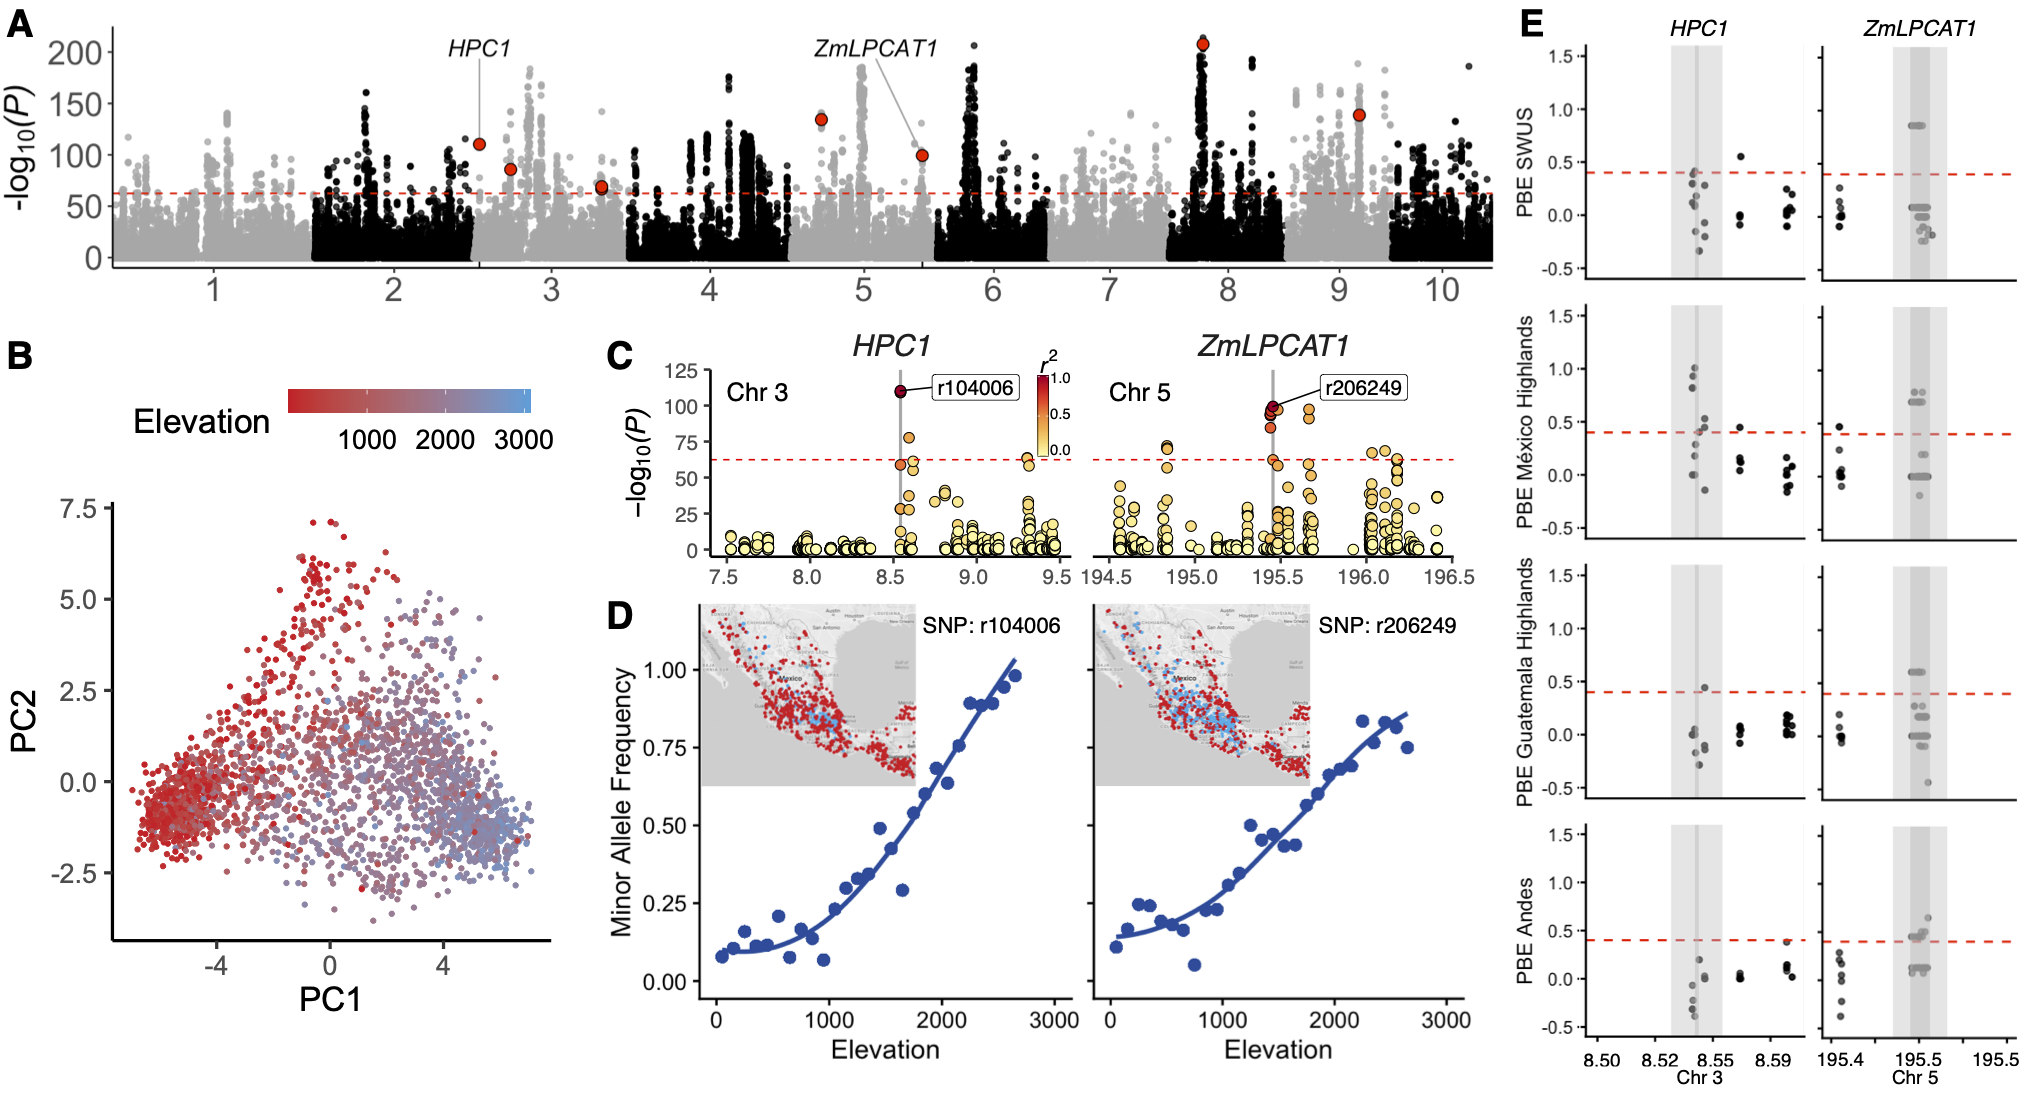
\includegraphics[width=0.8\paperwidth]{Chapter-1/figs/Fig_2.png}
\caption[Evidence of highland selection in genes determining PC/LPC ratios]{\textbf{\textit{Evidence of highland selection in genes determining PC/LPC ratios.}}
 \textbf{(A)} Association with genetic principal component 1 (PC1) from \textit{pcadapt} analysis of Mexican landraces (open pollinated varieties), dashed marks the top 5\% $-log_{10}(P)$. 
 Red points show SNPs in glycerolipid metabolism genes that are also PBE outliers for Mexican highlands (Supplementary Table 2). 
 From these, \hpc and \textit{ZmLPCAT1} are the top genes with orthologs catalyzing PC/LPC interconversion. 
 \textbf{(B)} Scatter plot of the \textit{pcadapt} first two genetic principal components illustrating that PC1 correlates with elevation.
 \textbf{(C)} Extended region from (A) of the 1 Mb interval around \hpc and \textit{ZmLPCAT1}. Linkage disequilibrium ($r^2$) with the peak SNP for each gene are illustrated by the color scale; both peak SNPs are located in the coding sequence. 
\textbf{(D)} Elevation clines for the peak SNPs from (C), the insets show the geographic distribution of the highland (blue) and lowland (red) alleles.
\textbf{(F)} Population Branch Excess of SNPs in \textit{ZmLPCAT1} and \hpc. Dark grey, coding sequence; light grey, 10 kb upstream and downstream; dashed line is the threshold for the top 5\% PBE value outliers.} 
\label{Fig2}
\end{figure}
\clearpage
We considered two possible explanations for the extent of convergent selection in highland populations (see explanations in \citep{Wang2020-mp, yeaman2018}). 
Adaptation may be conferred by a small number of genes, thereby imposing a \textit{physiological} constraint on the sources of adaptation leading to convergence. 
Alternatively, adaptation may be the result of many genes, but deleterious \textit{pleiotropic} effects restrict the number of genes that can be targeted by selection, also leading to convergence.  
Using Yeaman's $C_{hyper}$ statistic \citep{yeaman2018}, which quantifies these two modes of convergent adaptation, we determined that the overlap among putative adaptive genes in the four highland populations cannot be explained merely by physiological constraints ($C_{hyper} = 3.96$, Supplementary Table 1). 
A certain degree of pleiotropic constraint is therefore likely.
Overlap between adaptation candidates was higher for the SWUS, MH and GH population pairs ($C_{hyper} = 4.79$) than between the Andean and SWUS, MH and GH pairs ($C_{hyper} = 3.14$).

To further understand selection at the gene level, we used genotyping by sequencing (GBS) data from 2,700 Mexican maize landraces, generated by the SeeD project \citep{Romero_Navarro2017-cn, Gates2019-xu}, to run a \textit{pcadapt} \citep{Luu2017-ws} analysis to determine how loci might contribute to observed patterns of differentiation along major principal components of genetic variation. 
The first \textit{pcadapt} principal component separated Mexican landraces based on the elevation of their geographical origin (\cref{Fig2}B).
Using this first principal component, we identified outlier single nucleotide polymorphisms (SNPs) across the genome that are significantly associated with genetic variation along elevation and potentially involved in local adaptation (\cref{Fig2}A).
From the list of $\approx 600$ maize glycerolipid-related genes, 85 contained SNPs that were \textit{pcadapt} outliers for association with the first genetic principal component (top 5\% $-log_{10}(P)$), and of which eight were also PBE outliers for Mexican highlands (\cref{Fig2}A, Supplementary table 2, Sup. File 2). 
These eight selection candidates, supported by two different sources of evidence, included two genes coding for putative enzymes whose orthologs are known to directly catalyze PC/LPC interconversion reactions. 
The first gene, Zm00001d039542, with a $-log_{10}(P)$ of $110.28$, encoded a putative phospholipase A1 that we name \textit{High PhosphatidylCholine 1}, \hpc.
The second gene, Zm00001d017584, with a $-log_{10}(P)$ of $99.31$, encoded a predicted \textit{Lyso-Phosphatidylcholine Acyl Transferase 1} that we will refer as \textit{ZmLPCAT1}. (\cref{Fig2}C). 
Although these two types of enzymes catalyze broadly opposite reactions (degradation vs biosynthesis of PC) they are unlikely to catalyze strictly reverse reactions in the Lands cycle. 
A1 phopholipases attack the phosphatidylcholine at the \textit{sn-1} carbon, while LPC acyl transferases usually acylate \textit{sn-2} \citep{wang2012,richmond2011}.
Instead, plant PLA1 enzymes like \hpc are better known for their role in the first step of jasmonic acid biosynthesis \citep{wang2018b, Ishiguro2001-ob}.

\begin{figure}[!ht]
\centering
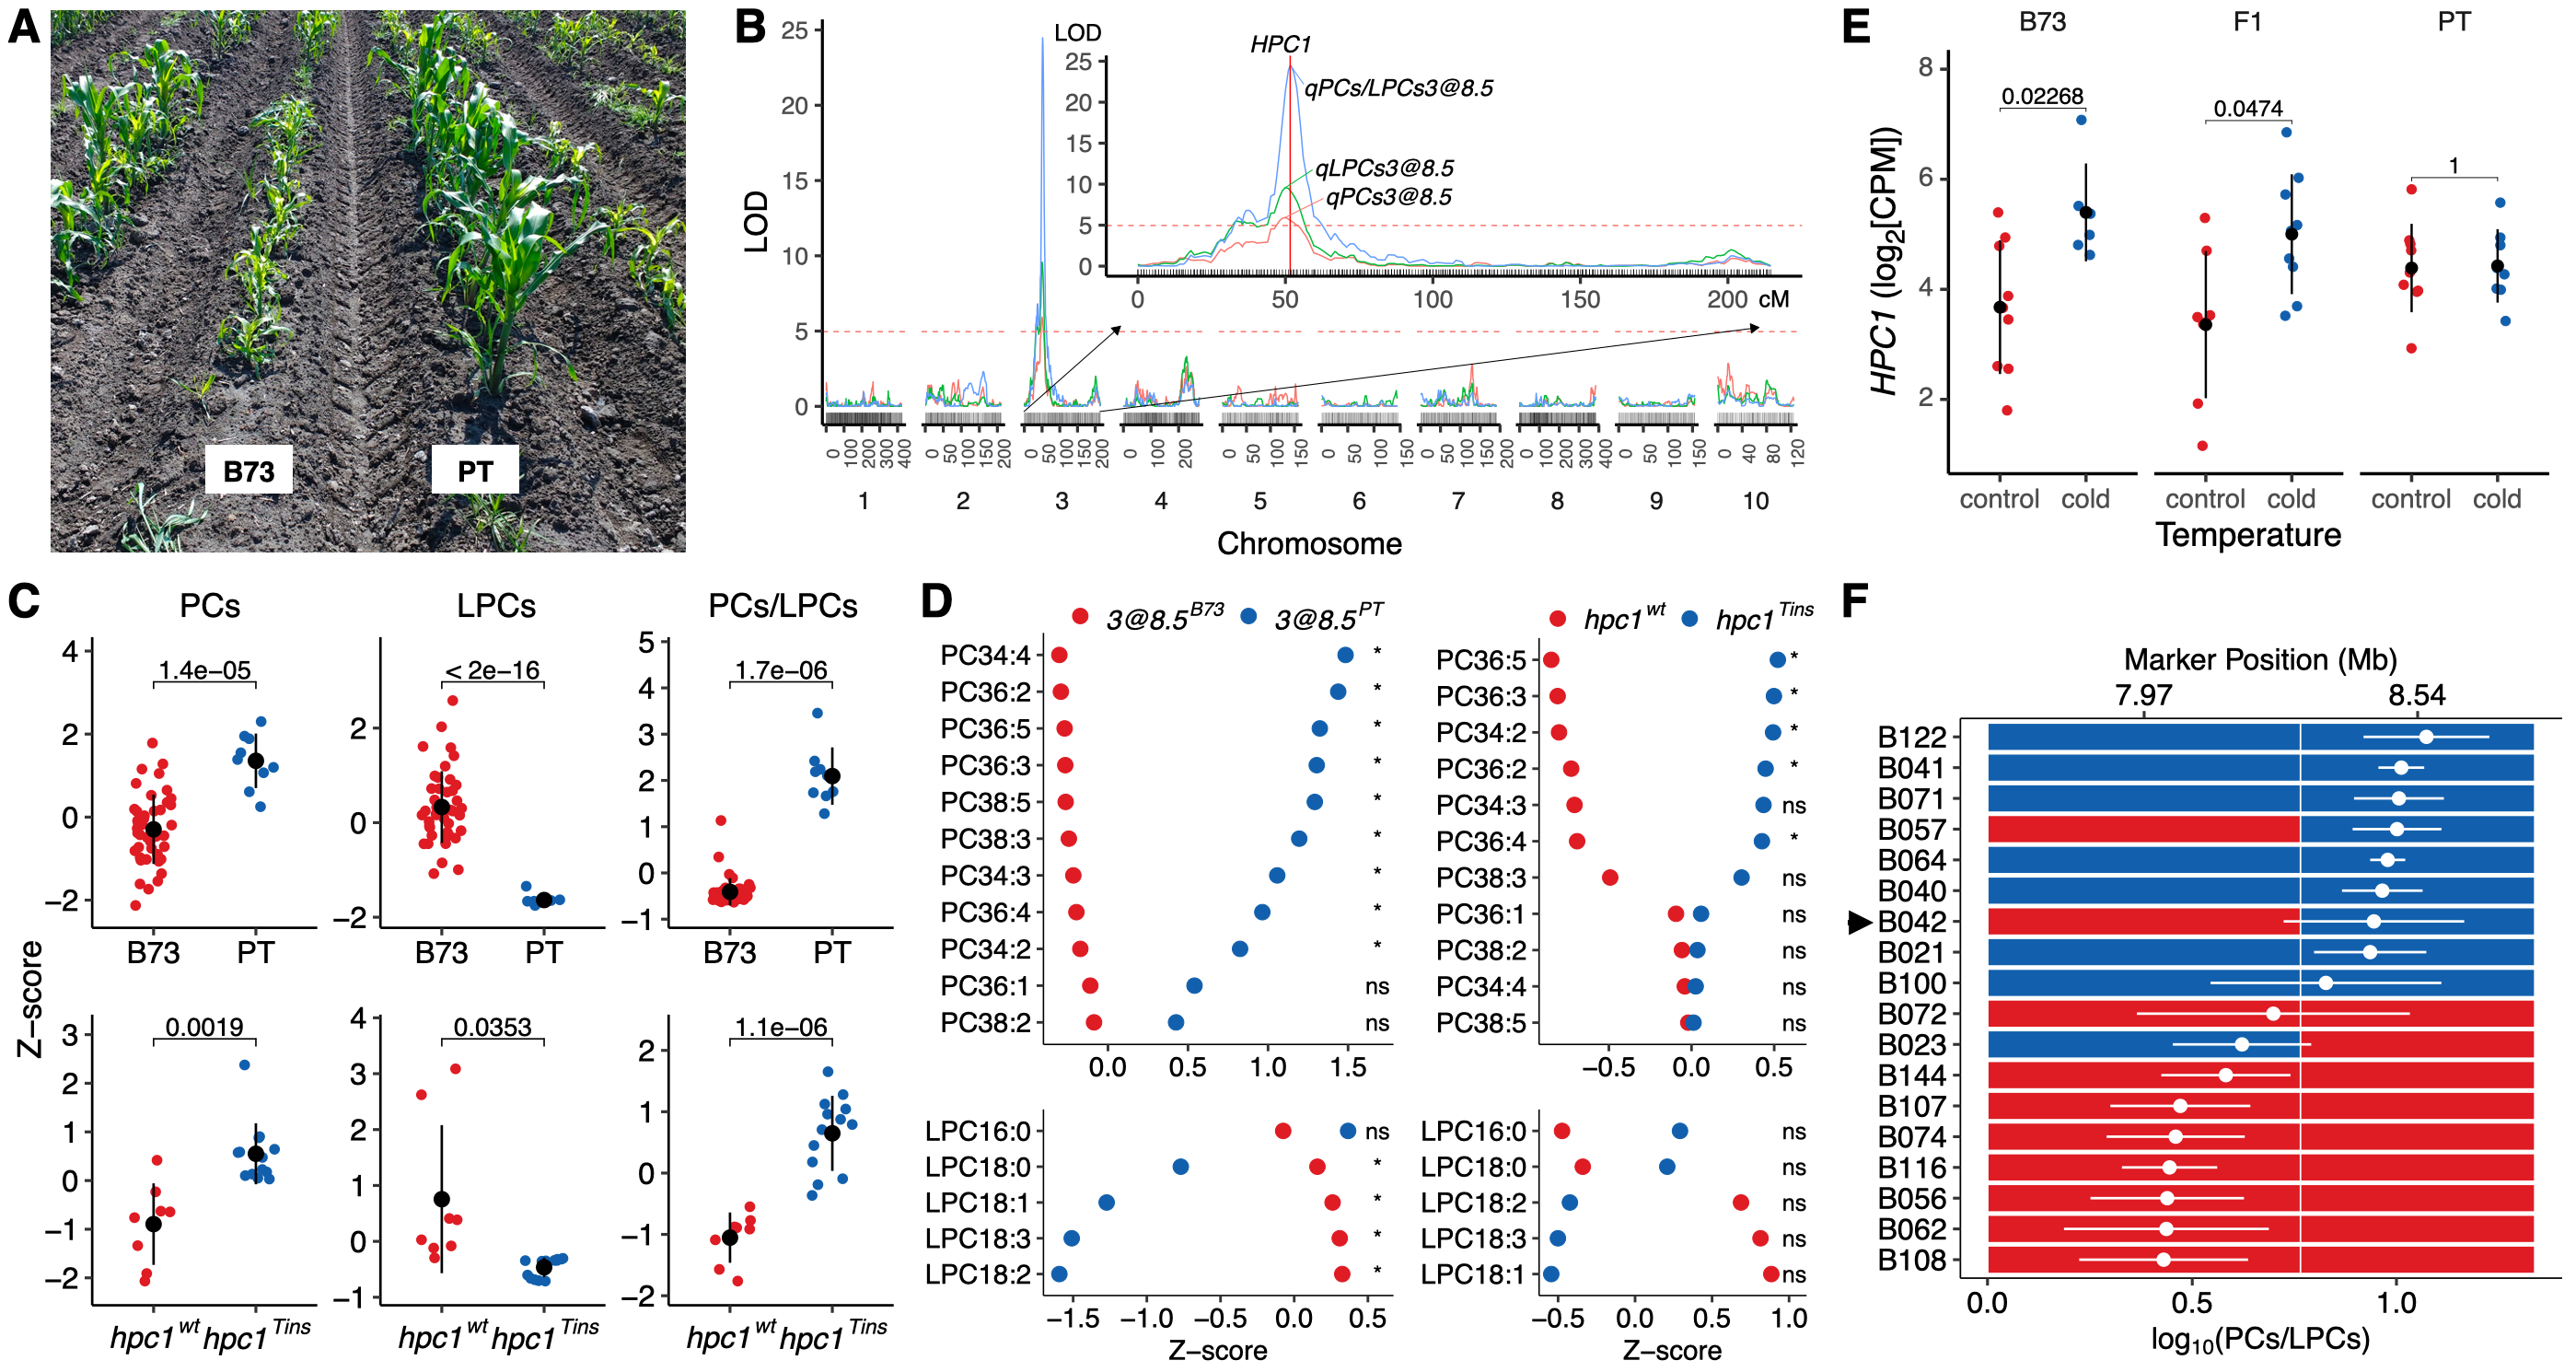
\includegraphics[width=0.8\paperwidth]{Chapter-1/figs/Fig_3.png}
\caption[\hpc defines a major QTL explaining PC/LPC conversion]{\textbf{\hpc defines a major QTL explaining PC/LPC conversion.} 
\textbf{(A)} PT and B73 plants growing in the highland Metepec field. 
\textbf{(B)} QTL analysis identified overlapping major QTLs around 8.5 Mb on chromosome 3 for PC and LPC levels and PC/LPC ratio, using data collected from plants grown in highland and lowland fields. 
The QTL peaks coincide with the physical location of \hpc. 
\textbf{(C)} Effect sizes for PCs, LPCs and PC/LPCs (z-score normalized) in RILs that are either homozygous for B73 or PT at 8.5 Mb on chromosome 3 (top row) and CRISPR-Cas9 \textit{hpc1\textsuperscript{Tins}} mutant and wild-type plants (bottom row).
Significant differences were tested by \textit{t}-test; the resulting \textit{p}-values are shown. 
\textbf{(D)} Effect sizes for individual PC and LPC species (z-score normalized) in RILs at 8.5 Mb on chromosome 3 (left) or the CRISPR/Cas9 \textit{hpc1\textsuperscript{Tins}} mutant (right). \textit{*} Significant difference at $p < 0.05$ (\textit{t}-test, after Benjamini \& Hochberg correction), \textit{ns} not significant.
\textbf{(E)} \hpc expression analysis in B73, PT and their F\textsubscript{1} hybrids grown in standard and cold temperatures in a growth chamber. Significant differences were tested by \textit{t}-test with Benjamini \& Hochberg correction; the resulting \textit{p}-values are shown.
\textbf{(F)} PC/LPC ratio for several RILs. RIL B042 (indicated by the black arrow) bears a recombination event 500 bp upstream of the \hpc translation start codon.
In panels (C-F), phenotypes associated with the B73 haplotype are in red; the equivalent values for the PT haplotype are in blue.}
\label{Fig3}
\centering
\end{figure}

Both genes showed strong changes in elevation-dependent allele frequency (\cref{Fig2}D) across Mexican landraces.
\hpc was not an outlier for branch excess between the Andean and the South American lowland accessions.
By contrast, \textit{ZmLPCAT1} was indeed a PBE outlier for all four populations, which may indicate parallel/convergent selection for this gene between Mesoamerican and Andean landraces.
Importantly, both \hpc and \textit{ZmLPCAT1} are annotated as part of pathways with outlier PBE values in all highland populations for ‘phospholipid remodelling’ and ‘PC acyl editing’ (Fig.\cref{Fig1}F, Sup. File 2). 
Taken together, these two independent population genetic approaches show that pathways involved in phospholipid remodelling,  including genes controlling the PC/LPC ratio like \hpc and \textit{ZmLPCAT1}, show strong selection signals in highland maize. 
These results indicate that selection on phospholipid metabolite levels (\cref{Fig1}B-D) is supported at the gene-level by outlier PBE and principal component analysis values \textit{pcadapt} in genes controlling phospholipid biosynthesis and degradation.

%%%%%%%%%%%%%%%%%%%%%%%%%%%%%%%%%%%%%%%%%%%%%%%%%%%%%%%%%%%%%%%%%%%%%%%%%%%%%%%%%%%%
\subsection{A major QTL explaining PC to LPC conversion overlaps \hpc}
%%%%%%%%%%%%%%%%%%%%%%%%%%%%%%%%%%%%%%%%%%%%%%%%%%%%%%%%%%%%%%%%%%%%%%%%%%%%%%%%%%%%
To further characterize the genetic architecture of phospholipid biosynthesis in highland maize, we developed a recombinant inbred line (RIL) BC1S5 population derived from a cross between the temperate inbred line B73 and the Mexican highland landrace Palomero Toluqueño (PT), using B73 as the recurrent parent (75\% B73, 25\% PT) \citep{Perez-Limon2022-lg}.

The parental PT accession is a popcorn landrace (\textit{palomero} means popcorn in Spanish) from the Toluca Valley in M\'exico (\textit{Mexi5} CIMMYTMA 2233) (\cref{Fig3}A). 
We grew the HiLo diversity panel and the B73 x PT BC1S5 RIL population in the same highland and lowland common gardens and collected samples for glycerolipid analysis.
The locally adapted PT landrace displayed higher fitness than B73 in the highland field (\cref{Fig3}A), probably due to adaptation to low temperatures in this highland environment.  
In the Mexican highlands, values of 5 GDDs per day are typical, while 15-20 GDDs/day are common in lowland environments. 


We detected major quantitative trait loci (QTLs) for the sum of LPC species levels, PC species levels, and the PC/LPC ratio that all mapped to the same locus on chromosome 3, around 8.5 Mb (\cref{Fig3}B). 
We tested for epistatic interactions for LPC levels, PC levels, and the PC/LPC ratio through a combination of R/qtl \code{scantwo} and \code{stepwise} functions \citep{Broman2003-ac}.
The three QTLs \textit{qLPCs3@8.5}, \textit{qPCs3@8.5} and \textit{qPCs/LPCs3@8.5} were robust against environmental effects and were detected in both the highland and lowland environments.
The additive effect of the PT allele at these QTLs was associated with high levels of PCs, low levels of LPCs, and consequently high PC/LPC ratios, while the B73 allele had the opposite effect (\cref{Fig3}C, top panel).
Individual PC and LPC species QTLs at this locus \cref{figure:Sup:QTL_effect_sp} showed the same additive effect for the PT allele as the sum of each class (PCs, LPCs, and PCs/LPCs) of species (\cref{Fig3}C, top panel. 
All individual LPC QTLs at the \textit{qLPCs3@8.5} locus corresponded to LPCs that contained at least one double bond in their fatty acid (\cref{figure:Sup:QTL_effect_sp}, Sup. file 3).
\textit{qPCs3@8.5} was driven mainly by PC species with more than two fatty acid double bonds, such as PC 36:5 (\cref{Fig3}D and \cref{figure:Sup:QTL_effect_sp} A-D, Supplementary file 3).
We then sought to identify candidate genes underlying the QTLs on chromosome 3.
The PC/LPC ratio QTL had the highest significance, with a logarithm of the odds (LOD) of 24.5, and explained the most phenotypic variance (87\%). 
The underlying QTL interval contained 72 genes within its 1.5 LOD drop confidence interval (7.9-10 Mb). 
We hypothesized that the metabolic phenotypes we observed might be due to a gene involved in PC-LPC conversion.  
The maize genome encodes 75 putative phospholipases (\cref{figure::Sup:HPC1_misc}A), of which half are predicted to be phospholipase A1-type (PLA1) (\cref{figure::Sup:HPC1_misc}B).  
Notably, \hpc mapped within the interval (position on chromosome 3: 8,542,107 bp to 8,544,078 bp), making it a high confidence candidate causal gene (\cref{Fig3}B). 
HPC1 was predicted to have phospholipase A1-Igamma1 activity and can be classified as a PC-hydrolyzing PLA1 Class I phospholipase based on its two closest Arabidopsis orthologs (encoded by \textit{At1g06800} and \textit{At2g30550}) \citep{Ryu2004-iv}. 
PLA1-type phospholipases hydrolyze phospholipids in the \textit{sn-1} position and produce a lyso-phospholipid and a free fatty acid (\cref{figure::Sup:HPC1_misc}B). 
In B73, \hpc was one of the most highly expressed phospholipase genes, with expression almost exclusively restricted to vegetative leaves (V4-V9) (\cref{figure:Sup:B73_expression}A) \citep{Stelpflug2016-vr}, which was the biological material we sampled for glycerolipid analysis. 
In B73 leaves, \hpc was also the most highly expressed gene within the QTL interval (\cref{figure::Sup:HPC1_misc}C) \citep{Stelpflug2016-vr}.
Class I phospholipases are chloroplast-localized proteins; in agreement, we identified a chloroplast transit peptide (CTP) at the beginning of the predicted HPC1 sequence using the online tool ChloroP \citep{Emanuelsson1999-rs}.
We validated the chloroplast localization of HPC1 by transiently expressing a construct encoding the HPC1 CTP fragment fused to green fluorescent protein (GFP) in \textit{Nicotiana benthamiana} leaves (\cref{figure:Sup:HPC1_organelle}).

The effect of \hpc on PC/LPC levels may be caused by misregulation of \hpc expression in highland landraces and/or by a mutation affecting HPC1 enzymatic activity. 
To distinguish between these two possibilities, we analyzed \hpc expression in B73, PT, and the corresponding F\textsubscript{1} hybrid plants grown at high and low temperatures to simulate highland and lowland conditions, respectively (\cref{Fig3}E). 
Under cold conditions, \textit{HPC1-B73} was up-regulated, but \textit{HPC1-PT} was not (\cref{Fig3}E). 
The lack of up-regulation in cold conditions of \hpc may explain the high PC/LPC levels in PT.
However, \hpc expressed to the same levels in B73 and PT under control conditions.
In the F\textsubscript{1} hybrids, \hpc expression was consistent with a dominant B73 effect.
We also observed a dominant B73 effect at the metabolic level when we analyzed B73 x PT RILs that are heterozygous at the \hpc locus
(\cref{figure::Sup:HPC1_misc}D).
Variation in \hpc may also affect enzymatic activity of the HPC1-PT variant. 
To test this hypothesis we sequenced three B73 x PT RILs (B021, B042, B122) that are homozygous for the \textit{HPC1-PT} allele.
We discovered a recombination point between 493 and 136 bp upstream of the \hpc translation start codon (\cref{Fig3}F, \cref{figure:Sup:hpc1_promoter}) in RIL B042, resulting in a chimeric locus with the coding region from PT combined with a promoter segment from B73.
PC/LPC levels in RIL B042 were similar to other RILs that are homozygous for the PT haplotype at the 8.54 Mb marker at the QTL peak (\cref{Fig3}F). 
This result supports the hypothesis that the metabolic effect in the B73 x PT RILs is likely due to an impaired function of the HPC1-PT enzyme rather than to changes in the \textit{HPC1-PT} regulatory region.
However, regulatory variants in the first 500 bp of the promoter may also impact expression levels in RILB042.

If \hpc is the underlying causal gene of this QTL, the observed metabolic phenotypes would be consistent with a reduction or loss of HPC1-PT enzyme function, leading to higher levels of PCs and lower levels of LPCs in the PT background. 
To test this hypothesis we generated mutants in \hpc via clustered regularly interspaced short palindromic repeats (CRISPR)/CRISPR-associated nuclease (Cas9)-mediated genome editing (\cref{figure:Sup:CRISPR_effect}A) in the B104 inbred, a temperate stiff stalk inbred derived from the Iowa Stiff Stalk Synthetic population like B73. 
We identified two transgenic mutants, hereafter designated \textit{hpc1\textsuperscript{CR T ins}} and \textit{hpc1\textsuperscript{CR T del}} (\cref{figure:Sup:CRISPR_effect}A).
We then measured PC and LPC species in wild-type and mutant plants grown under long day conditions.  
The phospholipid profiles of the \textit{hpc1\textsuperscript{CR}} plants 
replicated those of the \textit{PT} allele in the RILs (\cref{Fig3} C-D bottom panels and \cref{figure:Sup:CRISPR_effect}B), confirming that the \textit{HPC1-PT} allele impairs HPC1 function and thus underlies the QTL on chromosome 3 around 8.5 Mb. 
Lastly, we \textit{in vitro} translated HPC1-B73 and HPC1-PT  versions of the protein in a cell-free system and incubated them with various phospholipid substrates. 
We then measured the amount of phospholipid substrate and lyso-phospholipid product for each compound (\cref{figure:Sup:MS_spectra}). 
This experiment confirmed that both HPC1 variants have PLA1 activity and suggested that HPC1-B73 may have higher activity on substrates like PC36:4 that show stark differences in abundance between highland and lowland lines, as well as in \textit{hpc1\textsuperscript{CR}} lines.
Together, the RIL and CRISPR mutant results showed that \hpc underlies a major metabolic QTL explaining PC/LPC ratio. 
A mutation in the flap-lid domain of HPC1 affecting substrate accessibility likely leads to impaired function in the highland PT allele.

%%%%%%%%%%%%%%%%%%%%%%%%%%%%%%%%%%%%%%%%%%%%%%%%%%%%%%%%%%%%%%%%%%%%%%%%%%%%%%%%%%%%%%%%%%%%%%%%%%%%%%%% 
\subsection{\hpc shows strong elevation-dependent antagonistic pleiotropy in Mexican landrace fitness phenotypes}
%%%%%%%%%%%%%%%%%%%%%%%%%%%%%%%%%%%%%%%%%%%%%%%%%%%%%%%%%%%%%%%%%%%%%%%%%%%%%%%%%%%%%%%%%%%%%%%%%%%%%%$$
Our selection and QTL analysis provided strong evidence that \hpc is under selection in highland maize and controls phospholipid metabolism. 
To evaluate the possible fitness effects of HPC1 variation in locally adapted landraces across M\'exico, we re-analyzed phenotypic data from a previously reported F1 association mapping panel \citep{Romero_Navarro2017-cn, Gates2019-xu} composed of about 2,000 landrace F1s grown in 23 common garden environments across an elevation gradient.  
We then fitted a model to estimate the effect of variation at \textit{HPC1-PT} on the relationship between fitness traits and elevation \citep{Runcie2019-Gr}.
\hpc was a clear outlier in a genome wide association study (GWAS) of genotype-by-elevation fitness traits like flowering time and yield (\cref{figure:Sup:GxE_scan}A-B), indicating that elevation-dependent variation at \hpc not only has an effect on phospholipid levels but also on fitness traits.
Indeed, variation at \hpc showed significant genotype $\times$ elevation effects for several fitness traits (\cref{Fig5}A). 
The effect of \hpc on flowering time revealed antagonistic pleiotropy between highland and lowland environments (\cref{Fig5}A). 
The highland \textit{HPC1-PT} allele was associated in low elevations with delayed flowering, increasing days to anthesis (DTA) by about one day.
Meanwhile the same allele exhibited accelerated flowering at high elevation (with a decrease in DTA of almost one day, \cref{Fig5}A).
Variation at \hpc also displayed conditional neutrality on fresh ear weight and grain weight per hectare traits: the highland allele had no effect in lowland environments but was associated with greater values in highland environments (\cref{Fig5}A).
We also checked previous reports for associations between \hpc and flowering time in other populations through the MaizeGDB \citep{Woodhouse2021-wd} genome browser. 
We in fact found a significant flowering time SNP in the \hpc coding sequence (\cref{Fig5}B) for the Nested Association Mapping (NAM) population \citep{Wallace2014-yy}. 
This additive flowering time locus is only 6 bp from the focal SNP we used to test  $G \times E$ at \hpc in the SEEDs panel (\cref{Fig4}). 
Variation at this SNP correlated with a reduction in flowering time of 8.5 hours, relative to B73, and explained 1.12\% of the trait variance, which is about one third of the largest effect observed for flowering time variation in the NAM population. 

\begin{figure}[htp]
\centering
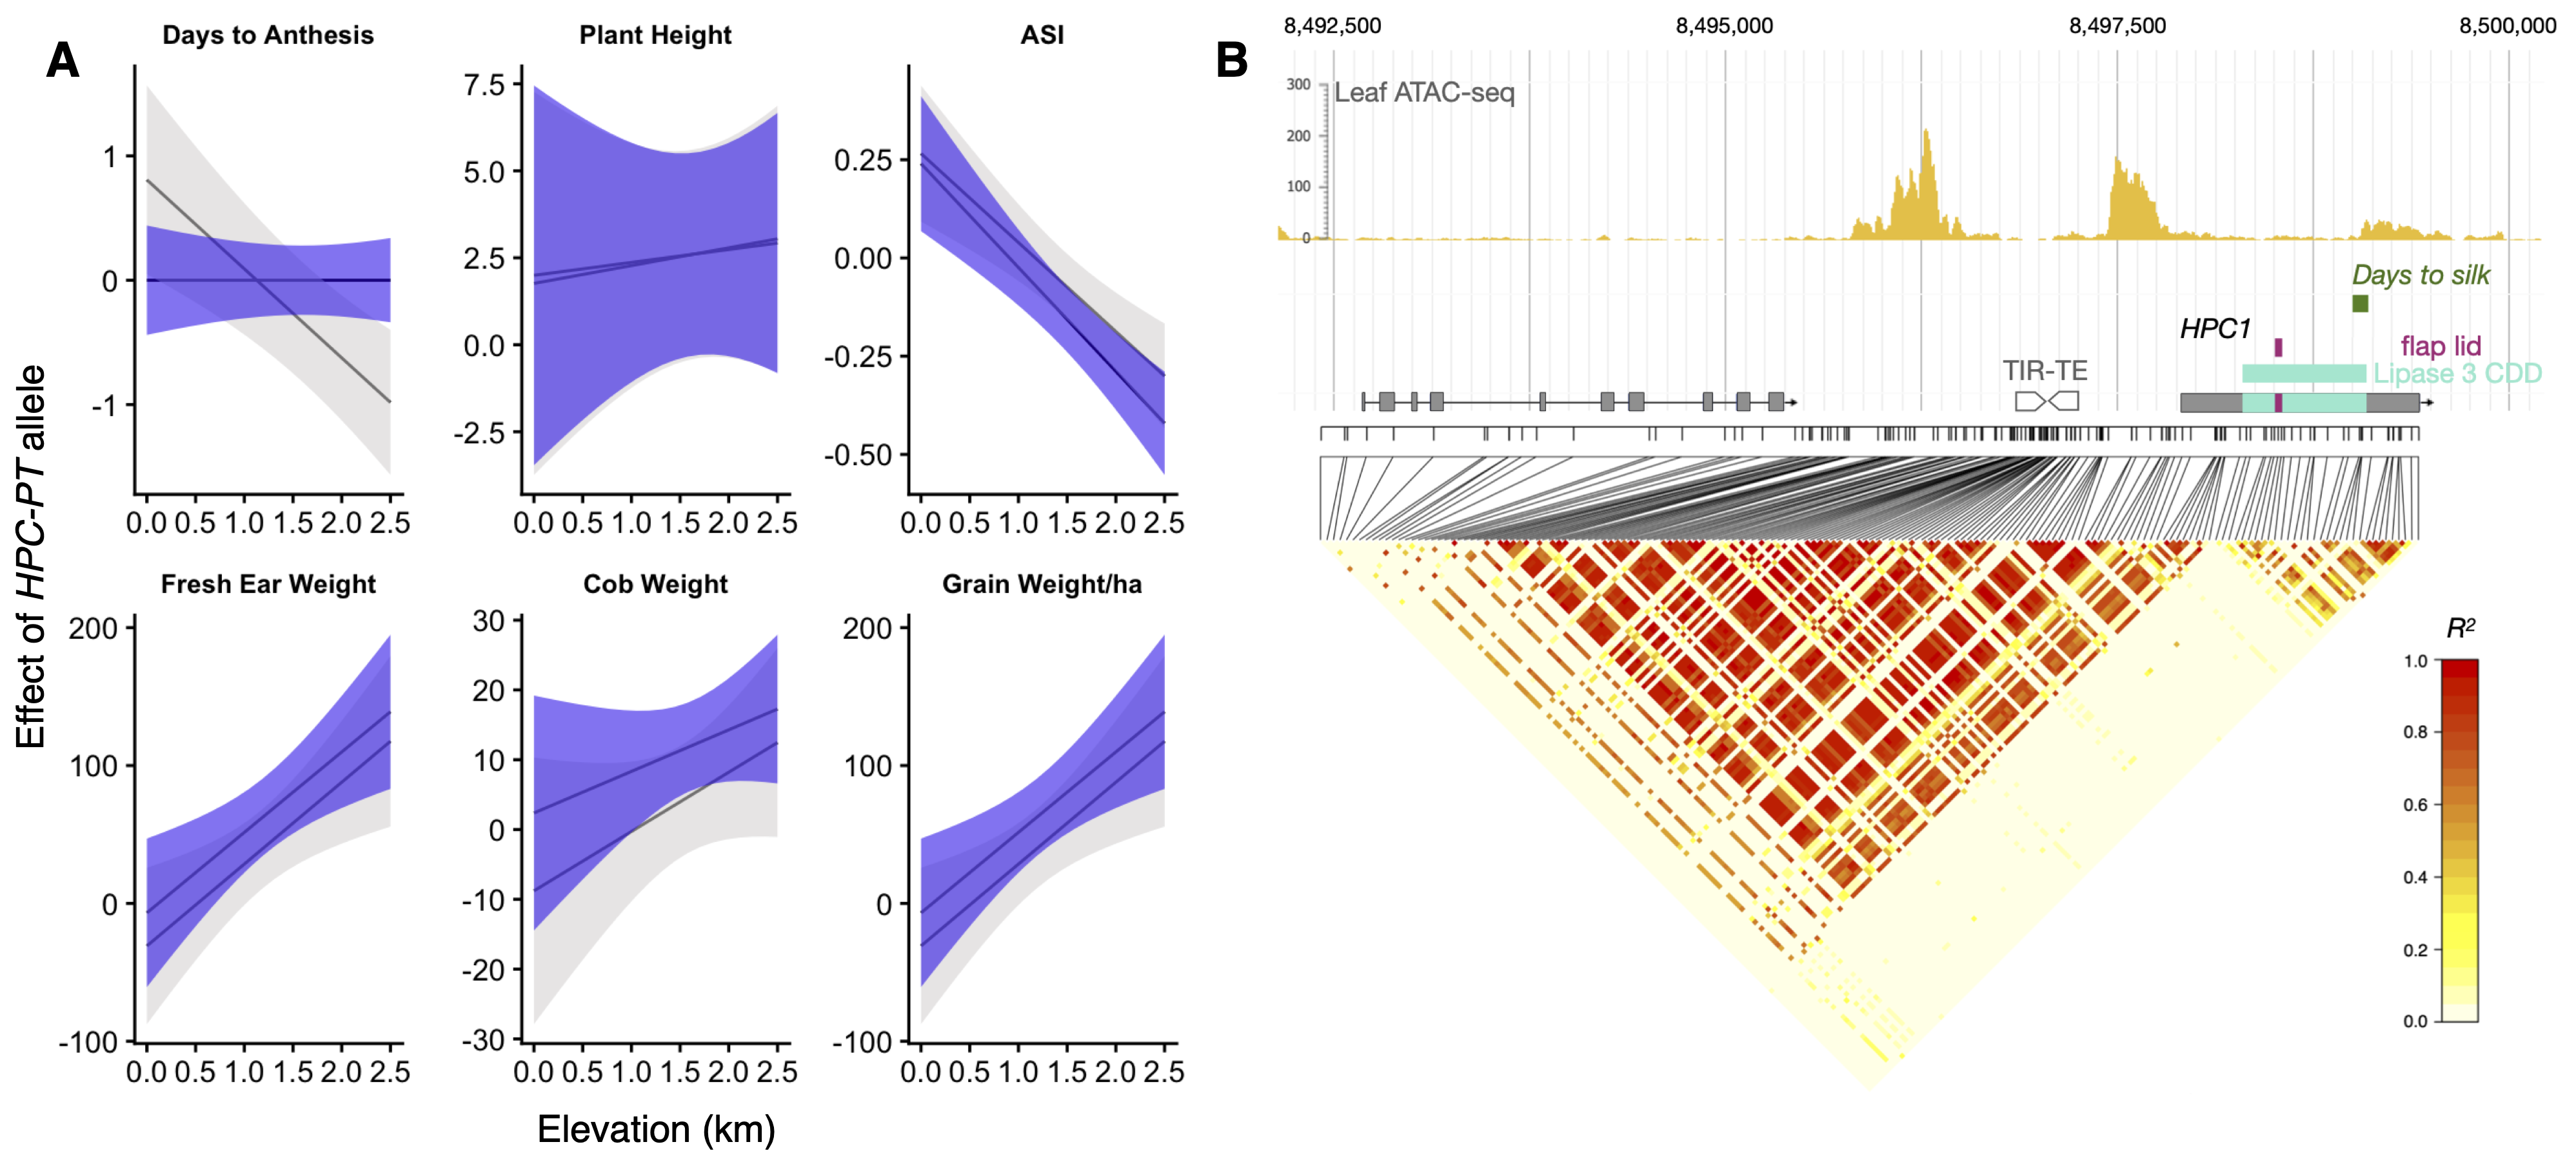
\includegraphics[width=0.8\paperwidth]{Chapter-1/figs/Fig_5.png}
\caption[Fitness effects of the \textit{HPC1-PT} allele and \hpc LD analysis.]{\textbf{Fitness effects of the \textit{HPC1-PT} allele and \hpc LD analysis.} \textbf{(A)}
We used best linear unbiased predictions (BLUPs) and GBS data from 2,700 landrace topcrossess from \citep{Gates2019-xu}, evaluated in 23 common gardens at different elevations in M\'exico. 
We modeled each trait as a function of the \textit{HPC1-PT} genotype, trial elevation, and tester line, with controls for main effects and responses to elevation of the genomic background. 
Gray lines and ribbons show estimates of the effect of the highland allele of \textit{HPC1-PT} as a function of common garden elevation ± 2 standard errors of the mean, using the \textit{GridLMM} package \citep{Runcie2019-Gr}. 
Purple lines show estimates of the \textit{HPC1-PT} effect in a model that also adjusts for effects of days to anthesis. ASI, anthesis to silking interval. 
\textbf{(B)} Linkage disequilibrium and genomic features of \hpc and upstream region. 
LD heatmap drawn with \citep{zhou2019} from HapMap 3 data. 
Top track shows leaf ATAC-seq peaks in B73, data from \citep{Ricci2019-zj}.
The regions coding for the lipase and flap-lid domains are highlighted on the \texit{HPC1} gene model. 
See \ref{Fig4}A for further details.
Days to Anthesis indicates the GWAS SNP on the lipase domain from \citep{Wallace2014-yy}.
TIR-TE, terminal inverted repeat transposable element.
Tracks obtained from MaizeGDB B73 V5 browser \citep{Woodhouse2021-wd}.}
\label{Fig5}
\end{figure}

We then used genetic marker data from the HapMap 3, which includes the NAM parents, \citep{Bukowski2017-ng} to analyze linkage disequilibrium (LD) of the \hpc region (\cref{Fig4}B).
We detected a strong LD block of about 150 bp in length in the coding sequence that includes the focal SNP mentioned above (\cref{Fig5}A,B). 
We identified another LD block covering the 5' region of \hpc and the promoter region up to 2 kb upstream of \hpc (\cref{Fig5}B). 
Interestingly, this second LD block on the promoter overlapped with two strong ATAC-seq (assay for transposase-accessible chromatin followed by sequencing) peaks identified in B73 (\citep{Ricci2019-zj}, \cref{Fig5}B).
These results confirmed that the SNPs associated with fitness traits like flowering time on the \hpc coding sequence are not linked to other SNPs upstream of the \hpc coding sequence.
However, the SEEDs data set lacks GBS markers for several kb upstream of \hpc, raising the possibility of a second regulatory variant in the promoter (\cref{Fig4}B) that might have an effect on \hpc expression. 
We further evaluated the possible effect of \hpc on flowering using both \textit{hpc1\textsuperscript{CR}} mutants in long-day conditions during the Summer of 2021 in Raleigh, NC. 
Although the mutants showed high PC/LPC ratios, we observed no significant difference in flowering time relative to the wild type (\cref{figure:Sup:CRISPR_effect}C). 
As shown in (\cref{Fig4}A) the effect of the \hpc allele on flowering time has a strong G x E pattern and we only observe a significant effect in very high or low elevations. 
We speculate that the absence of significant differences in the B104 CRISPR mutants in Raleigh conditions could partly be explained by the strong G X E effect of \hpc and/or genetic background effects. 

In summary, the SNPs in the short, lipase-domain-encoding LD block of \hpc show strong genotype x elevation fitness effects in both Mexican landraces grown across multiple altitudes and the NAM population.
The phospholipid changes induced by \hpc have physiological effects that may explain the strong selection of \hpc in highland environments.
%%%%%%%%%%%%%%%%%%%%%%%%%%%%%%%%%%%%%%%%%%%%%%%%%%%%%%%%%%%%%%%%%%%%%%%
\subsection{\textit{HPC1-PT} was introgressed from teosinte \mex and is conserved in Flint inbred lines}
%%%%%%%%%%%%%%%%%%%%%%%%%%%%%%%%%%%%%%%%%%%%%%%%%%%%%%%%%%%%%%%%%%%%%%
We explored the segregation of the V211I SNP among other highland maize varieties.
We detected the PT allele at high frequencies in highland landraces from M\'exico and Guatemala. 
In addition, the PT allele segregated in Southwestern US landraces. 
The B73 allele was fixed in lowland Mexican, South American, and Andean landraces (\cref{Fig6}A). 
These results were consistent with our PBE results (\cref{Fig2}F).
The PT allele was also present in one fourth of all teosinte \parv accessions tested and in both \mex accessions reported in Hapmap 3 \citep{Bukowski2017-ng} (\cref{Fig6}A). 
This observation prompted us to examine whether the PT allele was the result of post-domestication introgression from teosinte \mex during maize highland colonization, or whether it was selected from \parv standing variation.
To test for introgression from \mex, we used \(f_d\) data from \citep{Gonzalez-Segovia2019-jy} and established that the genomic region containing \hpc shows signatures of introgression from \mex into highland maize (\cref{Fig6}B).
We then performed a haplotype network analysis using SNP data from the \hpc coding region of 1,160 Mexican accessions from the SeeD Dataset \citep{Romero_Navarro2017-cn} that are homozygous for all SNPS across the coding region and the teosinte inbred lines (TILs) from Hapmap 3 \citep{Bukowski2017-ng}.   
We identified nine haplotype groups that cluster mainly based on elevation (\cref{Fig6}C). 
The two major groups, II and VI, contained mainly lowland and highland landraces, respectively. 
The two \mex teosinte inbred lines (TIL08 and 25) belonged to group IV  (\cref{Fig6}C) together with highland landraces primarily collected in the Trans-Mexican Volcanic Belt (30/36 from the highlands of Jalisco, Michoacán, M\'exico, Puebla, and Veracruz).
We then examined whether this \mex haplotype (denoted \textit{ZxHPC1}) that is introgressed into Mesoamerican highland maize was also present in modern maize inbred lines. 

To this end, we performed a neighbor-joining cluster analysis using Hapmap 3 \citep{Bukowski2017-ng} inbred lines including those from the 282 inbred panel, Teosinte inbred lines, German lines, and PT. 
We identified two main groups, one containing the \textit{HPC1-PT} haplotype and the other containing the \textit{HPC1-B73} haplotype.
PT and the teosinte \mex inbred lines TIL08 and TIL25 clustered together with Northern European Flint inbred lines such as EP1, UH008, and UH009 (\cref{Fig6}D). 
Other Northern US flints, e.g., CM7, were also closely related to the \mex \textit{ZxHPC1} haplotype. 
These data suggest that after introgression into highland maize, the \textit{ZxHPC1} haplotype was maintained in Flint materials adapted to cold environments in the Northern US, Canada, and Europe. 
We then used a large gene expression dataset consisting of multiple developmental stages of the 282-maize diversity panel \citep{Kremling2018-gn} and phenotypic datasets collected from the same panel grown in long days and short days.
Notably, \hpc expression levels were highly correlated with flowering time in both long and short days. 
Lines carrying the \textit{HPC1-PT} allele were characterized by lower \hpc expression and earlier flowering times relative to lines carrying the \textit{HPC1-B73} allele (\cref{Fig6}E).
Taken together, these data show that \hpc was introgressed from teosinte \mex into highland maize and that this introgression was carried over into high latitude-adapted modern inbred lines with low \hpc expression and early flowering.
\begin{figure}[!ht]
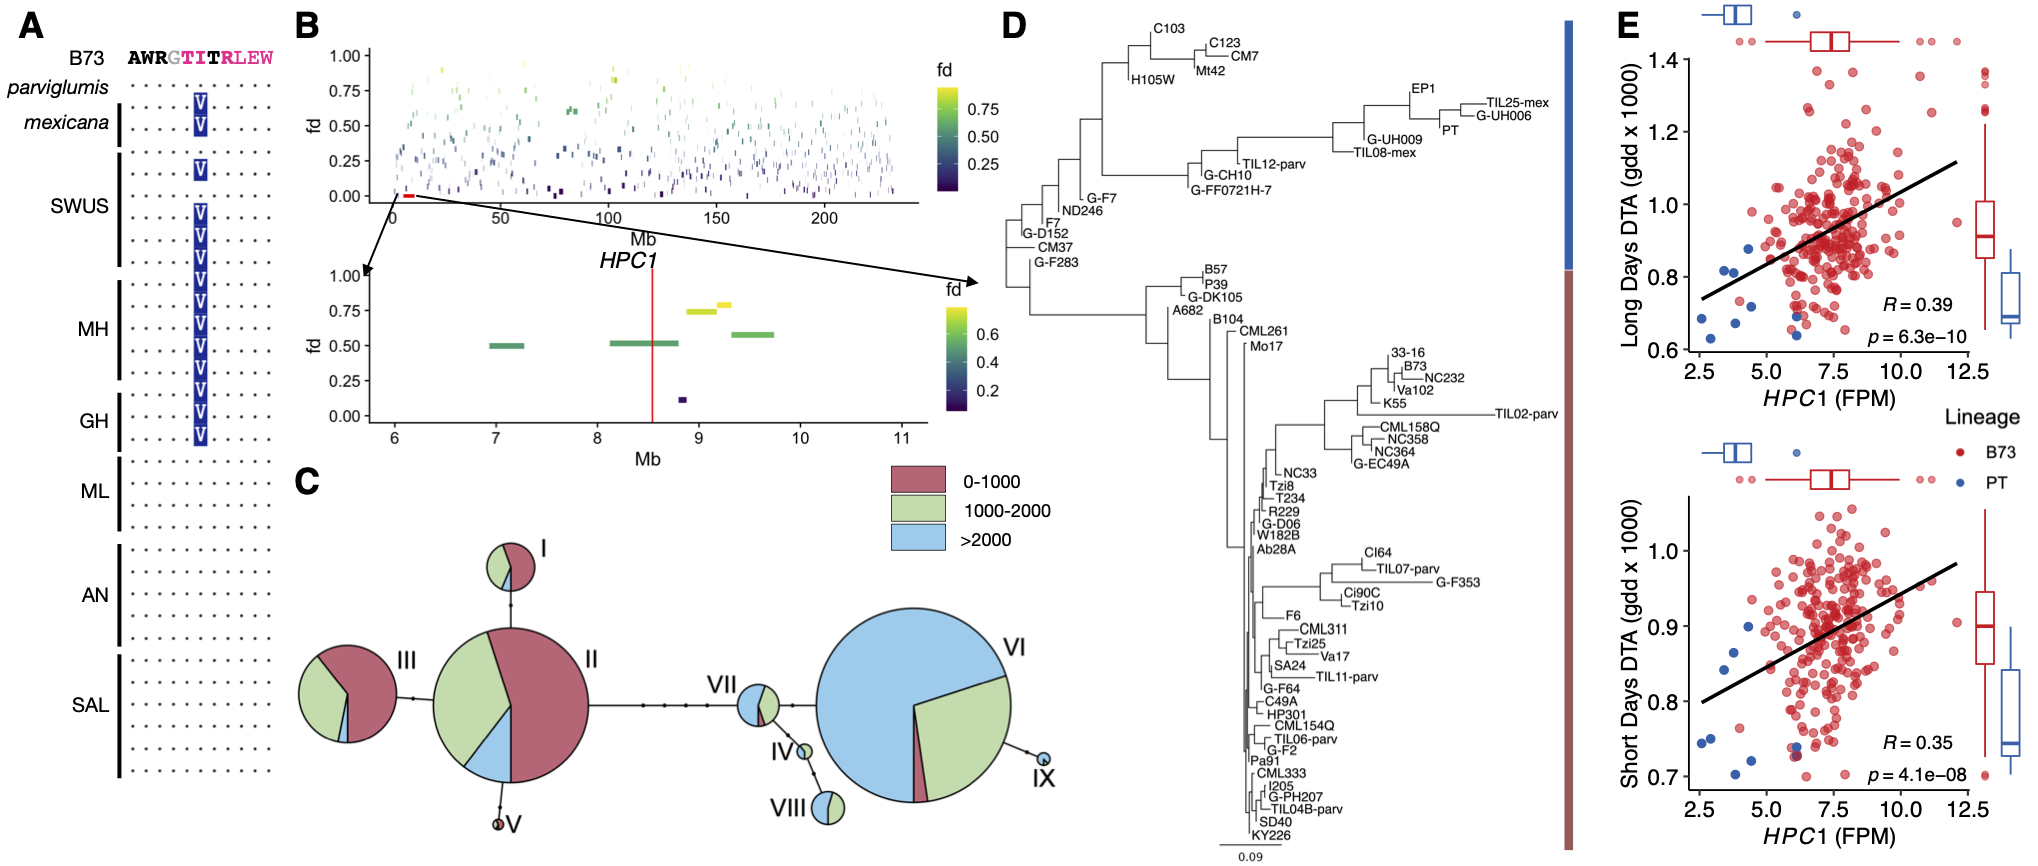
\includegraphics[width=0.8\paperwidth]{Chapter-1/figs/Fig_6.png}
\caption[Introgression of teosinte \mex into maize \hpc.]{\textbf{Introgression of teosinte \mex into maize \hpc.}  
\textbf{A)} Alignments around the V211I polymorphism in the flap-lid domain of HPC1 in B73, \mex and \parv and landraces of the Southwestern US (SWUS), Mexican Highland (MH) and Lowlands (ML), Guatemalan Highlands (GH), Andes (AN) and South America Lowlands (SAL).
\textbf{B)} \(f_d\) analysis of the \mex introgression. Data were obtained from \citep{Gonzalez-Segovia2019-jy}. 
\textbf{C)} Haplotype network analysis of SNPs within the \hpc coding region, using 1,060 Mexican homozygous individuals from the SeeD dataset. Haplotypes are color-coded by elevation: red: 0-1000 masl, green: 1000-2000 masl, blue >2000 masl.
\textbf{D)} Cluster analysis of the \hpc coding region using a sample of Hapmap3 inbred lines and the PT landrace.
\textbf{E)} Correlation between \textit{HPC1-PT} expression and days to anthesis (DTA) in plants grown in short or long days. 
Inbred lines from the PT lineage shown in panel C are indicated in blue and inbred lines from the B73 lineage are in red;
data from \citep{Kremling2018-gn}.}
\label{Fig6}
\end{figure}

\section{Discussion}

Understanding the genetic, molecular, and  physiological basis of crop adaptation to different environments and the role that wild relatives have played in these processes is relevant for the identification of favorable genetic variation that can be used to improve modern crops.
The repeated events of maize adaptation to highland environments constitute an excellent natural experiment to study local adaptation. 
Recent studies \citep{Wang2020-mp, Takuno2015-uj, Crow2020-gene} have helped expand our understanding of the genetic basis underlying maize highland adaptation. 
However, the responsible molecular, physiological, and genetic mechanisms underlying maize highland adaptation and the possible role of highland maize traits in modern, commercial varieties remain largely unknown.
Phospholipids are key structural components of plant membranes that also function as signaling molecules during adaptation to stresses that would be prevalent in highland environments \citep{Ryu2004-iv, Nakamura2017-vb} such as low phosphorus availability \citep{Veneklaas2012-ls, Cruz-Ramirez2004-ib, Lambers2012-an} and low temperatures \citep{Degenkolbe2012-wf, Welti2002-uk, Marla2017-ph}. 
In Arabidopsis and rice (\textit{Oryza sativa}, phospholipid species regulate flowering time via interactions with \textit{Arabidopsis} FT and rice Heading date 3a (Hd3a), respectively \citep{Nakamura2014-qf, Susila2021-dz, Qu2021-wc}. 
Flowering time is a major driver of maize adaptation to highland environments \citep{Romero_Navarro2017-cn, Gates2019-xu, Mercer2019-vj} and to northern latitudes \citep{Hung2012-ms, Swarts2017-ge}.

Genes involved in the biosynthesis and degradation of phospholipids appeared to have been repeatedly selected in several highland maize populations of North America, Central America, and South America (Figures \cref{Fig1} and \cref{Fig2}). 
\textit{ZmLPCAT1} and \hpc were two such genes with the strongest, repeated signals of selection, as measured by PBE and \textit{pcadapt} in highland populations (\cref{Fig2}). 
In a previous study, \textit{ZmLPCAT1} exhibited high $F_{ST}$ values when highland and lowland landraces were compared \citep{Takuno2015-uj}.
In temperate inbred lines, \hpc was up-regulated while \textit{ZmLPCAT1} was down-regulated by cold stress (\cref{figure:Sup:B73_expression}B-C) \citep{Waters2017-nat}.
These expression patterns are in agreement with the high and low PC/LPC ratios observed in our experiments. 
Furthermore, we determined here that \hpc is up-regulated in B73 and B73 x PT F\textsubscript{1} hybrids after cold exposure. 
By contrast, the \textit{HPC1-PT} and \textit{HPC1-B73} alleles were expressed to comparable levels in control conditions, and the \textit{HPC1-PT} allele was not induced upon cold conditions (\cref{Fig3}E).
Selection at these two loci is likely to have driven the high PC/LPC ratio we observed in highland Mexican landraces (\cref{Fig1}). 

Our QTL analysis of the PC/LPC ratios in a B73 x PT mapping population and in the \textit{hpc1\textsuperscript{CR}} mutant alleles demonstrates that the highland \textit{HPC1-PT} allele results in an enzyme with impaired function that alters highland Mexican maize PC metabolism, leading to higher PC/LPC ratios (\cref{Fig3}, \cref{figure:Sup:CRISPR_effect}B). 
Adaptive loss-of-function mutations can be an effective way to gain new metabolic functions in new environmental conditions \citep{Hottes2013-np}.
Taking advantage of the conserved lipase domain of HPC1 in bacteria, we used a new method that can identify how genetic variation in DNA regions encoding protein domains is correlated with optimal growth temperature of bacteria \citep{Jensen2021-iv, Jensen2021-zm}.
The probable causal SNP in HPC1 changed an amino acid in the flap-lid domain of HPC1 (\cref{Fig5}A) that may affect substrate  accessibility and/or substrate binding (\cref{Fig5}A). 
Indeed, the flap-lid domain has been the target of biotechnological modification for lipases \citep{Khan2017-ua}.
The region encoding the flap-lid domain was located at a recombination point that separates two clear LD blocks. 
The first LD block covered a 2-kb promoter region of \hpc and the first 600 bp of \hpc, while the second covered the rest of the \hpc coding sequence. 
In fact, this pattern is characteristic of selective sweeps that leave two LD blocks on either side of the adaptive mutation sweep \citep{Kim2004-pa}. 
LD analysis together with the open chromatin detected by ATAC-seq that overlaps the same promoter region (\cref{Fig4}B) and the correlation between \hpc expression and flowering time (\cref{Fig6}E) presented here suggest a possible transcriptional regulation of \hpc that may act additively with the coding sequence variation we described. 

Why were the metabolic changes induced by HPC1 variation selected for in highland maize?
PC metabolism is intimately connected to multiple stress responses and developmental pathways; alterations in PC amounts and PC/LPC ratios affect overall plant fitness.
The \textit{qPC/LPC3@8.5} QTL is driven by individual QTLs for PC and LPC species with high levels of unsaturated fatty acids (\cref{Fig3}D).
Several of these species, like PC 36:5 and LPC 18:1 (\cref{Fig3}D, Sup. File 3), have been shown to display similar patterns during Arabidopsis cold acclimation \citep{Welti2002-uk} and sorghum (\textit{Sorghum bicolor}) low temperature responses \citep{Marla2017-ph}.
PC 36:5 also showed high $Q_{ST}$ values when comparing highland and lowland landraces from both Mesoamerica and South America (\cref{Fig1}C-D, Sup. File 5).
In maize, \hpc expression is under the control of the circadian clock \citep{Khan2010-iv} with a peak at the end of the day. 
In Arabidopsis, highly unsaturated PC (34:3, 34:4, 36:5, 36:6) species increase in the dark \citep{Maatta2012-ip}. 
This peak in contents coincides in maize with low \hpc expression levels during the same dark hours \citep{Khan2010-iv}.
PC, and lipid metabolism in general, is also intimately connected to flowering time. 
For instance, PCs were shown to bind to Arabidopsis FT in the shoot apical meristem to hasten flowering \citep{Nakamura2014-qf, Nakamura2019-ht} by unknown cellular mechanisms. 
Similarly, PG species can sequester FT in phloem companion cells in low temperatures \citep{Susila2021-dz} and then release FT into the phloem later after temperatures increase, allowing FT reach the shoot apical meristem.   
In agreement with an effect of lipids on flowering time, overexpression of a gene encoding a secretory phospholipase D delayed heading time in rice \citep{Qu2021-wc}.
In line with a role for phospholipids in flowering, we established that genetic variation at SNPs within the region of \hpc encoding the lipase domain exhibits a strong interaction with elevation for the highland \textit{HPC1-PT} allele. 
This variation leads to a delay in flowering time in low elevations and an acceleration at high elevations, both of which close to one day in amplitude. 
Interestingly, the effect of the highland \hpc allele exhibited typical conditional neutrality in yield-related traits, with higher fitness conferred by the \textit{HPC1-PT} allele in highlands (\cref{Fig4}A). 
In the NAM population, we identified another SNP mapping to the region encoding the lipase domain that is associated with a hastening of flowering time by eight hours with respect to B73 \citep{Wallace2014-yy}, further supporting the role of \hpc in controlling flowering time. 
Analysis of \hpc CRISPR mutant alleles in the B104 background grown in Raleigh displayed a PC/LPC phenotype that mimicked the highland allele (\cref{figure:Sup:CRISPR_effect}A-B) but not a flowering time phenotype, probably due to the strong G x E effect of \hpc and/or genetic background effects. 

The strong G x E effect we observed in \hpc is similar to the well-known teosinte \mex introgression \textit{inv4m} \citep{Crow2020-gene}. 
In fact, our analysis showed that \hpc is indeed another introgression from teosinte \texit{mexicana} (\cref{Fig6}A-C). 
Recent analysis using sympatric teosinte and maize populations across elevation gradients in Mexico further supports the introgression of \mex at \hpc and shows that the \mex ancestry of \hpc increases at a rate of +0.079 per 100 m of elevation \citep{Calfee2021-mr}.
We further demonstrated that the \texit{mexicana} intogression at \hpc is conserved in high latitude-adapted Flint lines from both Europe and the USA (\cref{Fig6}D).
\textit{HPC1} in inbred lines carrying the highland \textit{ZxHPC1} \mex haplotype was expressed at low levels and resulted in earlier flowering (\cref{Fig6}E) \citep{Kremling2018-gn}.  

Adaptation to higher latitudes involved a reduction of photoperiod sensitivity and flowering time that enabled maize to thrive in longer day conditions characteristic of the growing season at high latitudes \citep{Hung2012-ms, Swarts2017-ge, Yang2013-lg, Huang2018-ga}.
Additive mutations in the regulatory region of the gene \textit{ZCN8} \citep{Lazakis2011-nq}, including a teosinte \mex introgression, lead to higher expression of \textit{ZCN8}, which contributes to maize adaptation to long days in temperate conditions \citep{Guo2019-pn}.
\textit{ZCN8} is a close ortholog of Arabidopsis \textit{FT}, whose encoding protein interacts with several species of phospholipids to modulate flowering time \citep{Nakamura2014-qf, Susila2021-dz}. 
A similar interaction was also demonstrated for the rice FT ortholog Hd3a, \citep{Qu2021-wc} and we hypothesize that the same may be occurring in maize. 
Comparison of docking simulations of phospholipids with ZCN8 using the Arabidopsis FT crystal structures as a model \citep{Nakamura2019-ht} showed similar PC interactions in ZCN8 (\cref{figure:Sup:Docking}).
We corroborated this interaction via mass spectrometry analysis of lipids bound to ZCN8 heterologously produced in yeast (\cref{figure:Sup:ZCN8-PC}). 

In summary, we used a combination of genomic scans, linkage mapping, lipidomics and reverse genetics to identify and clone the adaptive gene \hpc, introgressed from teosinte  \mex, in highland maize landraces. 
HPC1 variants lead to a major reorganization of phosphatidylcholine metabolism. 
We showed that the fitness advantage conferred by the \hpc highland \mex allele is due, at least in part, to its association with flowering time. 
This effect may have contributed to adaptation of maize to colder, higher latitudes.

Our work is the first to identify the important role of a gene controlling phospholipid metabolism in plant local adaptation and further supports the emerging role of phospholipid metabolism in fine-tuning flowering time across different plant species \citep{Nakamura2014-qf, Susila2021-dz, Guo2019-pn}.
This study highlights the largely underappreciated role of highland maize and highland teosinte \mex in modern maize.

\printbibliography[heading=subbibintoc, title=References,]

% \chapter{Gene Discovery through Plant Genome Environment Associations:
The Case for Enhanced Machine Learning Models of Global Soil Phosphorus Availability}
\label{chap-two}

\newrefsection

\section{Abstract}

\section{Background}

\section{Methods}
\subsection*{Building and Validating a Model of Global Plant Available Phosphorus Distribution }

To find associations between soil phosphorus environment and the genetic diversity of crops, we first compiled public datasets on global phosphorus distribution and improved upon them using random forest models.
We aimed to  build a global model for two plant available phosphorus parameters. Soil phosphorus content as extracted with the Olsen method (Olsen1950); And Soil phosphorus as extracted with the Bray method 1 (Bray1950).
We intended at first to use the Olsen predictions by( Mcdowell 2023), but the correlation for LAC and African soil profile samples was close to 0 (Supplementary Figure 1). So we decided to refine the predictions by partitioning the global model in two, one model for each, the Nothern hemisphere (latitude >35) and one for the Southern hemisphere (latitude <= 35).
We used a set 20000 non-redundant georeferenced soil measurements, and interpolations,  for Olsen and  25000 profiles for Bray as compiled by McDowell2023. 
Then we retrieved maps for 15 predictors of available phosphorus as described by (He2020).The predictors were as follows: Mean Annual Temperature and Mean Annual Precipitation from BioClim 2.0 (FickHijmas2017); pH, soil organic carbon, bulk density, WRB soil groups and  USDA taxonomy big groups from SoilGrids 250 (Hengl2019, Hengl2017, WRB2023, USDA2015), biomes fom resolve Ecoregions (Dienerstein2017), Mean Annual Net Primary Production from MODIS (Running \& ZHao 2015), slope and elevation from EarthEnv (Amatulli2018), soil depth  from Land-Atmosphere Interaction Research Group (Shangguan2017), and lithology from GLiM(Hartmann2012) (details on Suplementary file S1).
The different map files we curated and matched in resolution and projection, so that at the end we have 15 10km (0.8883 x0.9993 decimal degrees) latitude longitude WGS84 rasters. To not give  overwhelming regression leverage to datapoints in long tails of skewed distributions, the predictors with heavily skewed distributions to the right were transformed  with log2, as were the two outcome variables, and then back transformed following Mcdowell2023.
We prefered to use this limited amount of covariates as their prediction value, computation time savings, and interpretability have been shown by He2020. 
Then we filled the gaps in the predictor variables for the Mcdowell Samples by using the highest resolution raster possible.
After this we aimed for building two independendent models for the northern and southern datasets. We used the R package Random Forest (randomf2020) with default hyperparameters, but including subsampling strata  for each of the Geo3 Major regions and getting an ensemble model out of 15 rounds of replication, with 4 fold cross validation (70\% training data, 30\% testing data). 
The two ensemble models were then used to make global predictions at 10 km resolution on their own domains (North vs South) and merged in a single raster.
Given the the local lack of sampling in Africa and Latin America, we checked the correlation of our Olsen and Bray Models with other proxies of available phosphorus in those regions, which are expected to correlate given their similar chemistry. The correlation of  our model predictions were checked with 1) In the case of Africa a model of water soluble phosphorus measured by mass spectrometry, isDASOIL (Miller2021, Hengle2017a) and  extractable phosphorus with the Hedley method in the case of Latin America and the Caribbean (Hou2019). 

To measure linear correlations between distinct previously reported phosphorus parameters and our model predictions, we transformed  each parameter according to their distributiion (Supplementary table 2)  and  added logit transformed probabilities of  soil phosphorus retention class from (Batjes2011).

Because of the crops used in this study we were interested in confirming that our plant samples were collected from soils that had reasonable predictor space overlap with the training data. For this we used a Factor Analysis dimensionality reduction approach, and did a MANOVA test for differences between the crop groups and the South Data set on this projection of the covariate space.

\subsection*{inv4m plant population, growth conditions,experimental design and phenotype measurements}

\subsection*{RNAseq tissue sampling, RNA extraction and Sequencing}

\subsection*{Differential Expression Analysis}

\subsection*{Gene Regulatory Network Analysis}

\subsection*{Lipid Analysis}

\section{Results}
\subsection{Enhanced Global Model of Olsen and Bray Phosphorus improve accuracy for the Southern Hemisphere}
After building on the work of He2020 and Macdowell2023, we increased the predictive value of the soil mapping models for Olsen and Bray extractable phosphorus in the Southern hemisphere. Our two hemisphere model increased the Pearson correlation $r$ from 0.0 to 0.7 (0 and 0.5 R2) for observed and predicted values of Olsen P, and  from 0.0 to 0.84 (0 to 0.7 R2) for observed and predicted values of Bray P (Observed-Predicted correlations table 1) in the Southern data.  [Compare mean squared root error]. In addition to this we see good overlap with the training data set for both Africa and LAC (Figure 1C) (MANOVA test), which allows us to make reasonable interpolations. A similar approach increased the total phosphorus predictive value as well from 0.81 to 0.91 (0.65 and 0.81 R2), marginally improving previously reported data for Africa (Hengl2017a), where we expect even less over-fit because of the better sampling and increased mixing of data points in the predictor space.

Appart from the predictive value,  the relative importance of  predictors in our models is congruent with the chemical understanding of how phosphorus goes into soil solution.
Phosphorus in solution depends on pH and soil mineralogy, while the total amount of phosphorus in non fertilized soils should depend mostly on parent material and organic mater fractions.
Thus the random forest predictor importance as measured by \%IncMSE in our small model is easier to understand than models including multiple multispectral vegetation indices and climate variables (Mcdowell).

This lead us to conclude that we have a more parsimonious model that has better prediction value and better interpretability.

Not only our model shows acceptable and improved internal consistency, but it has increased correlations with other reported measurements of available P. For example for the LAC pixels corresponding to the Hou sampling of Hedley available phosphorus the correlation between our Olsen is 0.5  and Bray is 0.4. For the Africa isDASOIL extractable phosphorus is 0.4.
At the level of continental and global models our Bray and Olsen predictions have high correlation with McDowell Olsen at the global scale but not in the southern hemisphere, with the predicted water soluble phosphorus in Africa (Miller2021, Hengl 2017a) and low correlations with previous raster values based on heuristics models like Shangguan 2017, Yang 2014 and Batjes2011 retention probabilities (Table1 other prediction correlations).

Although not comparable with prediction values for mean annual temperature (R2 = 0.98 Bioclim) our model improves prediction for Latin America (Macdowell) and previous models of Africa (Hengl 2017a) of plant available phosphorus.
Now with the best estimators we had of plant available phosphorus for plants in acicidic and basic soils we proceeded to look for Genome Environment Associations in two crops: Maize heirloom varieties in Mesoamerica and And Sorghum heirlooms in Africa.


\subsection{Maize Vegetative and Reproductive Traits have a marked response to Phosphorus but no detectable difference between Inv4m alleles(karyotypes) nor  Inversion x Phosphorus interaction}

We see a clear shoot phenotypic response to phosphorus treatment independently of Inv4m karyotype. 
Plants grown in low phosphorus grow slower and reach maturity later with a similar effect in both Inv4m and B73 homokaryotpes. 
The effect of phosphorus treatment is significant for all the vegetative growth measurements taken, plant height at anthesis, dry mass at 40, 50, 60 and 120 DAP.  
For reproductive traits low phosphorus leads to earlier time to male and female flowering, greater cob width and length, and a reduced yield as measured by total kernel weight per ear.
A closer analysis of the growth curves inferred from accumulated dry mass at different days show increased final dry mass  with increased phosphorus, a faster mass acquisition rate, and faster time to mid mass in higher phosphorus. 
There is slight evidence for an interaction between inv4m karyotype and growth. 

The standard homokaryotype (B73), seems to be more responsive to increased concentration of phosphorus in the soil, while the  inverted homokaryotype [inv4m] seems to not to lose as much dry weight in the low phosphorus treatment compared with high P input [make pairwise bootstrap test for the diference of means]. 
This behavior matches the expectation of B73 being selected for yield under high input agriculture in contrast with the Mexican Highland landraces that are selected for more predictable yields under variable stresses. In a phenotype PCA of the different mean row measurements the first dimension explaning 28\% of the variance with morphological phenotypes has weights associated with flowering time and dry mass accumulation, highlighting these variables as the most responsive to the phosphorus treatment (PCA biplot). 
The samples in this pheotypic ispace show a clear separation by treatment  but not  inv4m karyotypes ( 2 x MANOVA 2 groups) or their interaction (MANOVA 4 groups).

\subsection{Maize leaf expression shows a marked response to Phosphorus and Inv4m polymorphism, with some genes responding to Inversion x Phosphorus interaction}

At v8-9 maize plants showed a remarkable response to phosphorus in their leaf gene expression.
An multidimensional scaling of the gene expression shows an overall response to phosphorus that tends to increase with leaf-age and is associated with  the first dimension (Figure). 
While the second dimension shows more separation between samples due to leaf age.

After a mashr analysis for the effects of phosphorus treatment in gene expression we see that mir399 is consistently over-expressed from the most apical to the most basal of the sampled leaves.
Gene expression on target genes like SPX transporters were also consistently diminished in high phosphorus, corresponding to the overall expected response to phosphorus (mir2020).

There is a genome-wise effect of the phosphorus treatment on gene expression, as shown by the mashr p-values {expression manhattan plots}. We found a total of 10000 differential expressed genes (out of 20000 genes detected in at least one leaf sample), with a distrubution mostly consistent with gene density throughout the genome. 
In contrast, the effect of inv4m is mostly detected inside the boundaries of inv4m [I need to genotype the samples  show the actual boundaries  in these plants] with a  transcription factor being the most significantly affected gene in the group (cite fold change gene id predicted function).
We detected 300 genes that undergo inv4m effect in cis, while 300 genes show significant diferential gene expression in trans between inv4m karyotypes.
The mean magnitude of the effect in cis is greater than the mean effect in trans (mean fold value of the two grops, t-tes p value (sperate hypothesis for over and under expressed genes?)).

However the variation at inv4m seems to have no major effect in the gene response to phosphorus.
As shown by the mashr test for the Inversion x Phosphorus interaction there are 150 genes that have a differential response to phosphorus depending on the inv4m karyotype, with (20) genes in cis and (x) genes in trans.
A single gene close to inv4m shows a different response  to phosphorus (look for the id, check if it is in the inv4m) depending on inv4m genotype (show interaction plot).

Gone ontology and pathway analysis. 
We observe clear over representation of nitrogen associated biological processes and metabolic pathways in  the 10000 genes responsive to phosphorus treatment.
However when we reduce he list to the top 1000 most significant, the over represented gene processes and terms are more related to phosphorus (adjusted FDR < 1e-6). 
Meaning that the genes that show the greater and/or more consistent effect  have phosphorus associated funcions while nitrogen related genes are making significant but smaller adjustments in expression (t test for difference in effects between phosphorus genes and nitrogen genes), maybe reflecting cross-talk between phosphorus and nitrogen homeostasis (i.e nutrient interaction) (Vlad2022, other) [look for NxP imporrtant genes in vlad lists and other papers]. [I could mention the NEU results too]
[Make lists for over and under represented genes, maybe Miami plots?, a heatmap and hierarchical clustering of genes exprerssion profiles from leaf 1 to 4 might be nice use cheng li package to get a quick idea]

Genes that are deferentially expressed  due to Inv4m effect do not show over representation of either biological processes or pathways, not even when separated in induced vs repressed genes.
And, similarly, genes that show inv4m X phosphorus interaction in gene expression lack any specific functions statisttically associated either in Gene Ontology or Metabolic pathway database.

Overall there is no hard evidence from this transcriptome experiment that inv4m contributes to local adaptation to phosphorus, in the sense that it's adaptive contribution does not depend on phosphorus amount in the the soil.
However it is clear that inv4m plants reach faster time to maturity, and have less yield penalty under extreme phosphorus stress.
We could not find signals of photosynthesis or carbohydrate over representation in the Inv4m responsive to inversion karyotype, as was previously foundd in respons to cold (Crow2021) 


\subsection{Phosphorus response of the leaf gene regulatory network to inv4m introgrression}
\section{Discussion}


\printbibliography[heading=subbibintoc, title=References,]
\chapter{A highland maize chromosomal inversion decreases flowering time in a phosphorus-independent manner and leads to a minor perturbation of the leaf phosphorus starvation response transcriptome.}
\label{chap-three}
\newrefsection

\section{Abstract}
\invfour is a chromosomal inversion commonly found in traditional maize varieties grown in the Mexican highlands. 
\invfour was introgressed into cultivated maize from highland teosinte mexicana, and its highland predominance points to its contribution to local adaptation. 
In growth chamber experiments, \invfour-highland has been shown to regulate the expression of photosynthesis genes in response to cold.
In addition to cold, phosphorus is a limiting factor for plant growth in the Mexican highlands. 
In this study, we tested whether \invfour-highland contributes to local adaptation through an enhanced response to phosphorus deficiency. 
First, we bred Near Isogenic Lines (NILs) in B73 containing \invfour-highland introgressed from MICH21, a traditional Mexican maize variety, with the purpose of isolating the effect of \invfour-highland in a single, common genetic background.
Then we grew the \invfour-highland and control lines in the field under phosphorus sufficiency and deficiency. 
We measured flowering time, morphological traits, and leaf gene expression with RNA-seq. We found that independent of soil phosphorus status, \invfour-highland NILs flowered faster and grew taller than the controls while maintaining grain yield. 
There was a genomewide transcriptomic response to available phosphorus, affecting 7373 differentially expressed genes (DEGs), with the largest effect shown by \textit{PILNCR1-miR399}, a PSR regulator. The effect of \invfour-highland is narrower, affecting 528 DEGs, mainly within the boundaries of the inversion. The \invfour perturbation of PSR is limited to 1 DEG, the putative aldehyde dehydrogenase \textit{aldh2}. 
Our results confirm the contribution of \invfour to adaptation, as faster flowering, but we don’t find evidence of its effect on PSR.

\section{Background}

Chromosomal inversions might contribute to local adaptation by capturing locally adapted genotypes of several loci and limiting subsequent recombination \citep{kirkpatrick2006b}. 
In a Mexican diversity panel of maize traditional varieties (TVs), a chromosomal inversion in the chromosome 4, \invfour, was associated both to elevation and flowering time \citep{romero_navarro2017-cn}. 
More specifically, \invfour shows a classical pattern of gene-by-environment interaction produced by local adaptation: plants with the \invfour-highland allele have delayed flowering at low elevations and earlier flowering at high elevations \citep{crow2020}. 
The highland haplotype of \invfour was introgressed from \textit{Zea mays spp.} \mex \citep{calfee2021-mr,gonzalez-segovia2019-jy,hufford2013-gs} which is a maize wild relative native to the Mexican highlands. 
The \invfour inversion spans 13 Mb \citep{pyhajarvi2013, calfee2021-mr}, shows recombination repression, low genetic diversity, has clinal dependency on elevation, and is almost fixed at locations higher than 2500 m.a.s.l (\autoref{fig::design} A and B), \citep{crow2020,gonzalez-segovia2019-jy}. 
In a precedent work, \citep{crow2020}, \invfour-highland was shown to up-regulate the expression of photosynthesis genes in response to cold in seedlings. 
But cold is not the only limiting factor for plant growth in the highlands.
Andosols are volcanic soils that are almost exclusive to the highlands, in Mexico 95\% of natural andosols profiles are present above 2000 m.a.s.l, (calculated from \cite{paz-pellat2018,inegi2013}). 
Due to their vitreous nature andosols have high phosphorus retention, \citep{krasilnikov2013}, and tend to have low amounts of phosphorus available for plant uptake, \citep{galvan-tejada2014}.
MICH21 one of the accessions tested by \citep{crow2020}, is native to the Purépecha Plateau, where both, andosols \citep{paz-pellat2018,inegi2013,galvan-tejada2014}, and phosphorus use efficient maize TVs are usual \citep{bayuelo-jimenez2011, bayuelo-jimenez2014}. 
\invfour might contribute to faster growth in the highlands by carrying alleles that are beneficial during phosphorus starvation response (PSR).
In this study, we investigate whether \invfour-highland contributes to local adaptation through an enhanced response to phosphorus deficiency.
Here we use a more advanced generation of the Mi21-derived sub-population assyed by \citep{crow2020} for testing the effect of \invfour in the gene expression response to cold.

\begin{figure}[!ht]
\centering
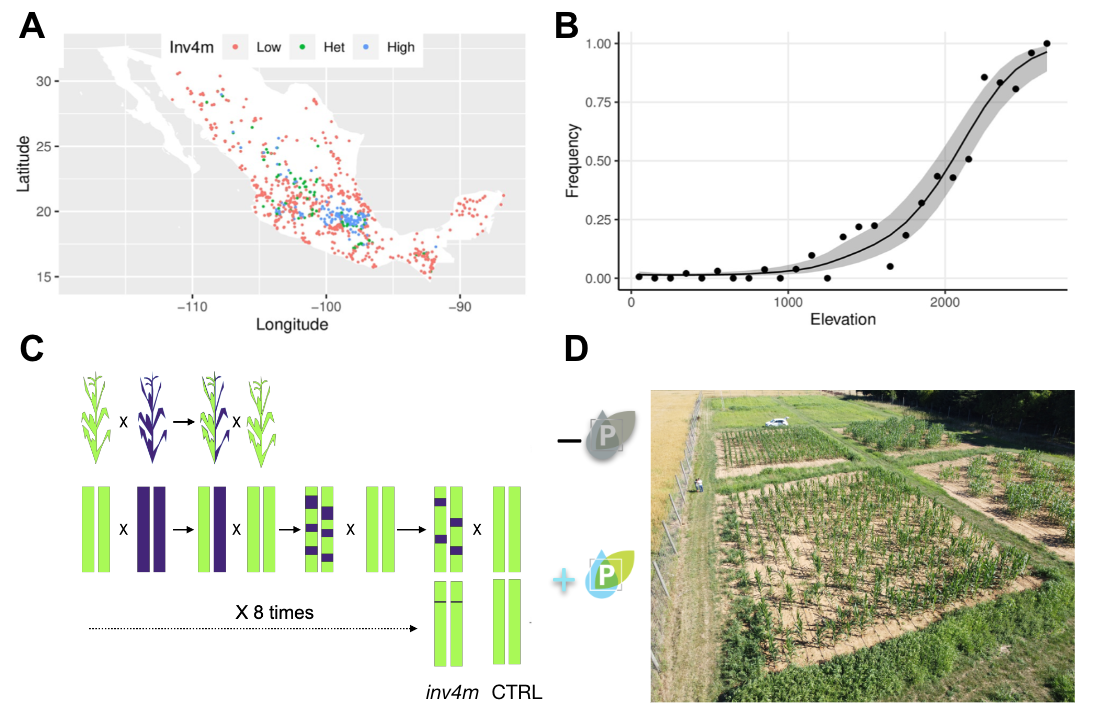
\includegraphics[width=\linewidth]{Chapter-3/figs/design.png}
\caption[\textit{\invfour} Distribution and Introgression Breeding Design]{\textit{\textbf{\invfour Distribution and Introgression Breeding Design.}} [A and B reproduced from \cite{crow2020}] \textbf{(A)} Distribution of lowand homozygous (Low), heterozygous (Het), and highland homozygous individuals of \invfour in Mexican traditional varieties.
\textbf{(B)} \invfour Allele Frequency Cline with Elevation in 100m bins.
\textbf{(C)} Near Isogenic Line breeding scheme, see details in methods, lines in the experiment are BC$_6$S$_2$.
\textbf{(D)}  Rock Springs, Pa, field station experimental setup.
}
 \label{fig::design}
\end{figure}

\section{Methods}
\subsection{\invfour plant population, growth conditions, experimental design, and phenotype measurements}

To measure the effects of the \invfour in plant field phenotypes and their phosphorus starvation response transcriptome, we used a highland traditional variety carrying the Highland haplotype of \invfour corresponding to the inverted karyotype.
The accession Michoacán 21 (referred to as Mi21), from the Mexican Cónico group, was obtained from the International Maize and Wheat Improvement Center (CIMMYT). 
In contrast, the reference genome of the temperate inbred B73, the recurrent parent for introgression, carries the lowland haplotype corresponding to the standard non-inverted karyotype at \invfour.

From the cross of Mi21 with B73 one F1 individual was backcrossed to B73 for six generations. During each cycle, we selected lines carrying  \invfour with a diagnostic SNP using a cleaved amplified polymorphic sequence (CAPS) marker. 
The marker SNP is PZE04175660223 located at position 4:181637780 in the NAM v5 \textit{Zea mays} genome assembly.
Amplification of the polymorphic site was done with the following primer pair: CTGAGCAGGAGATGATGGCCACTC and GGAAAGGACATAAAAGAAAGGTGCA, and subsequently cleaved by \textit{HinfI}.
Plants were genotyped using the CASP marker for selecting heterozygous plants at BC6S2 after selfing seeds of \invfour and CTRL homozygous individuals were selected for the field trial.


Plants were planted on May 26 2022 at the Russell E. Larson Agricultural Research Farm in Rock Springs, Pennsylvania (40°42’36" N 77°57’0" W, 366 m.a.s.l.) in soil classified as a Hagerstown silt loam (fine, mixed, semiactive, mesic Typic Hapludalf).
Experimental conditions were similar to previously described \citep{strock2018}. 
The experiment had a complete block design with two phosphorus (P) levels. 
Low-P fields (5 ppm Melich-3 Phosphorus)  and  high-P fields (36 ppm Melich-3 Phosphorus) were divided into smaller blocks. 
Three rows per block were planted with a mean stand count of 8 plants per plot, and the plants from the center row were selected for measurements to avoid border effects. Fields received fertilization based on treatment requirements. 
Drip irrigation was provided during dry periods. 
Each genotype was replicated four times within its P treatment.


\subsection{Phenotype analysis}

For stover mass growth curves, a different plant at each time point 40, 50, 60, and harvest, 121 days after planting (DAP), was collected, dried, and weighed for the same row. Stover dry mass data was fitted to a logistic growth model using the R package `growth curves`.
Maximum Stover dry weight was estimated to be the maximum over the four time points and not dry weight at harvest.
Ear measurements were taken for one ear per row at harvest. 

Phenotypes were modeled with thee R `lm` function as a multivariate multiple regression with fixed effects in the form of:

$$Y_{ijk} = \mu+ \beta_{1}C_{ijk} + \beta_{2}P_j+ \beta_{3}  \text{\invfour}_k+ \beta_{4} [\text{P} \times \textit{\text{\invfour}}]_{ij} + e_{ijk}$$.

with 

$$e_{ijk}\sim \mathcal{N} (0, {\sigma}^2)$$

For each phenotype $Y$, we modeled a response from the covariates $C_{ijk}$, that include row, column and block, $P_{i}$  the phosphorus treatment, $\text{\invfour}_{j}$ the \invfour genotype,  $[\text{P} \times \textit{\text{\invfour}}]_{ij}$ the genotype by treatment interaction term, and $e_{ijk}$ the residual for each replicate $k$, normally distributed with  mean zero and  variance $\sigma^2$.
Multiple hypothesis correction for the  t-test of model coefficient was done with a false discovery rate (fdr), and significant effects were reported below fdr = 0.05. 

\subsection{RNAseq tissue sampling, RNA extraction and Sequencing}
We took tissue samples 63 DAP when plants were between v7 to v9 developmental stages. 
Ten disc samples from the first leaf with a fully developed collar and every other leaf below for a total  of  four sampled leaves   per plant which where numbered 1-4 from apical to basal (\autoref{fig::RNAseq} A). 
Tissue was fast frozen in 1.5 mL tubes with two steel beads precooled with liquid nitrogen and kept in dry ice until stored at -80oC.
Four replicate plants were sampled per combination of  P treatment and \invfour genotype for a total of 64 tissue samples. 
I extracted total RNA with QIAGEN RNAeasy Plant Mini Kit  RNA extraction kit following manufacturer procedures (QIAGEN 74904), and RNA samples were quantified in nanodrop and sent to the NCSU Core Genomics Facility.
Following QC in bioanalyzer, Illumina libraries were prepared and sequenced in a lane of Novaseq according to manufacturer recommendations.


\subsection{Differential Gene Expression Analysis}
I aligned reads to the maize B73 NAM v5 genome using Kallisto \citep{bray2016}.
The alternative transcript alignment was turned into counts per gene per MB. We then used  voom  to calculate variance according to gene expression levels and counts were converted to log2(CPM). Then a  multivariate multiple regression between expression was run on each of the leaf positions, using the following model in limma :

$$Y_{ijk} = \mu + \beta_1 P_{ij}+ \beta_2 \text{\invfour}_{ij}+ \beta_3 [\text{P} \times \textit{\text{\invfour}}]_{ij} + e_{ijk}$$

with 

$$e_{ijk} \sim \mathcal{N} (0,\phi\sigma^2)$$

Linear model coefficients t-test p values were adjusted as false discovery rates, genes whose effect had a fdr <0.005 were deemed to be differentially expressed.
R scripts and expression data are  available at the  \href{https://github.com/sawers-rellan-labs/inv4mRNA}{\texttt{inv4mRNA} github repository}.



%\subsection*{Gene Regulatory Network Analysis}

%\subsection*{Lipid Analysis}



% \subsection{Phosphorus response of the leaf gene regulatory network to \invfour introgression}

\section{Results}

\subsection{Vegetative and reproductive traits had a marked response to phosphorus treatment and \invfour, but there is no  \invfour $\times$ P interaction effect}

I found a clear phenotypic response to phosphorus treatment independently of \invfour genotype ($\beta$ t-test, $\textrm{fdr} < 0.05$ ). 
Plants grown in low phosphorus grow slower and reach maturity later, with a similar effect in both \invfour and CTRL plants (\autoref{fig::effects} A). 
The effect of phosphorus treatment is significant for all the vegetative growth measurements taken, plant height at anthesis, and dry mass at 40, 50, 60, and 120 DAP.  
Plants growing in low phosphorus had faster male and female flowering times, greater cob width and length, and a reduced yield as measured by total kernel weight per ear (\autoref{fig::effects} B).
A closer analysis of the growth curves inferred from accumulated dry mass on different days showed an increased maximum stover dry mass in high phosphorus conditions, a faster mass acquisition rate, and a shorter time to mid-mass in higher phosphorus (\autoref{fig::growth}). 
There is slight evidence for an interaction between \invfour karyotype and growth. 

In a phenotype PCA of the different mean row trait values the first dimension explains 28\% of the variance. with morphological phenotypes has weights associated with flowering time and dry mass accumulation, highlighting these variables as the most responsive to the phosphorus treatment (PCA biplot). 
The samples in this phenotypic space show a clear separation by treatment but not  \invfour karyotypes ( 2 x MANOVA 2 groups F test, p < 0.05) or their interaction (MANOVA 4 groups, F test, p > 0.05).


\begin{figure}[!ht]
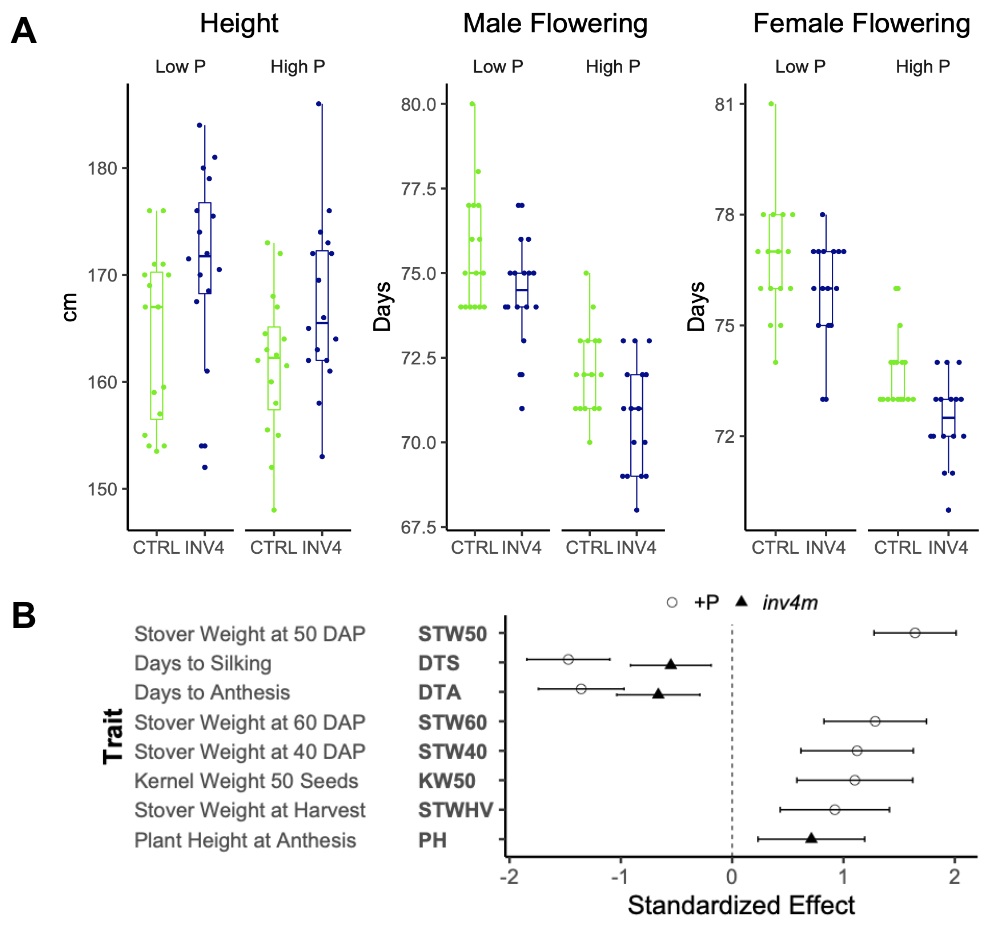
\includegraphics[width=\linewidth]{Chapter-3/figs/effects.png}
\caption[\textit{\invfour} plants flower earlier and are higher independent of phosphorus treatment]{\textit{\textbf{\invfour plants flower earlier and are higher independent of phosphorus treatment}}
% \\\hspace{\textwidth} 
\textbf{(A)} Distribution of traits where \textit{\invfour} genotype has a significant effect. ( Multivariable Multiple regression F test, fdr $<0.05$)
\textbf{(B)} Phosphorus treatment (circle), shows the greatest number of significant effects on traits, and larger absolute magnitude, compared to the \textit{\invfour} effect (triangle). Multivariable Multiple regression effect estimation mean $\pm$ 95 percent confidence interval (whiskers).}
\label{fig::effects}
\end{figure}


\begin{figure}[!ht]

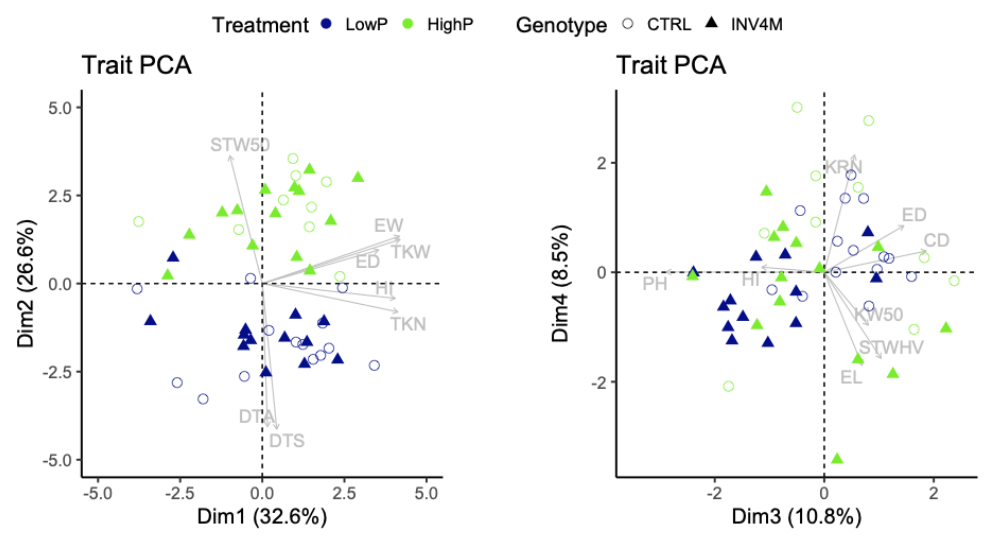
\includegraphics[width=\linewidth]{Chapter-3/figs/traitPCA.png}
\caption[Trait PCA showing that the effect of Phosphorus treatment dominates phenotype differences.]{\textbf{\textit{Trait PCA showing that the effect of Phosphorus treatment dominates phenotype differences.}}
% \\\hspace{\textwidth} 
\textit{Left:} Dim2, whose main contributors are Stover weight at 40 days after pollination, Days to Anhesis, and Days to Silking, sharply separates plants by phosphorus treatment. \textit{Left:} There is a slight separation by \textit{\invfour} genotype along Dim3, and especially along the Ear Diameter projection on this plane}
\label{fig::traitPCA}
\end{figure}

\begin{figure}[!ht]
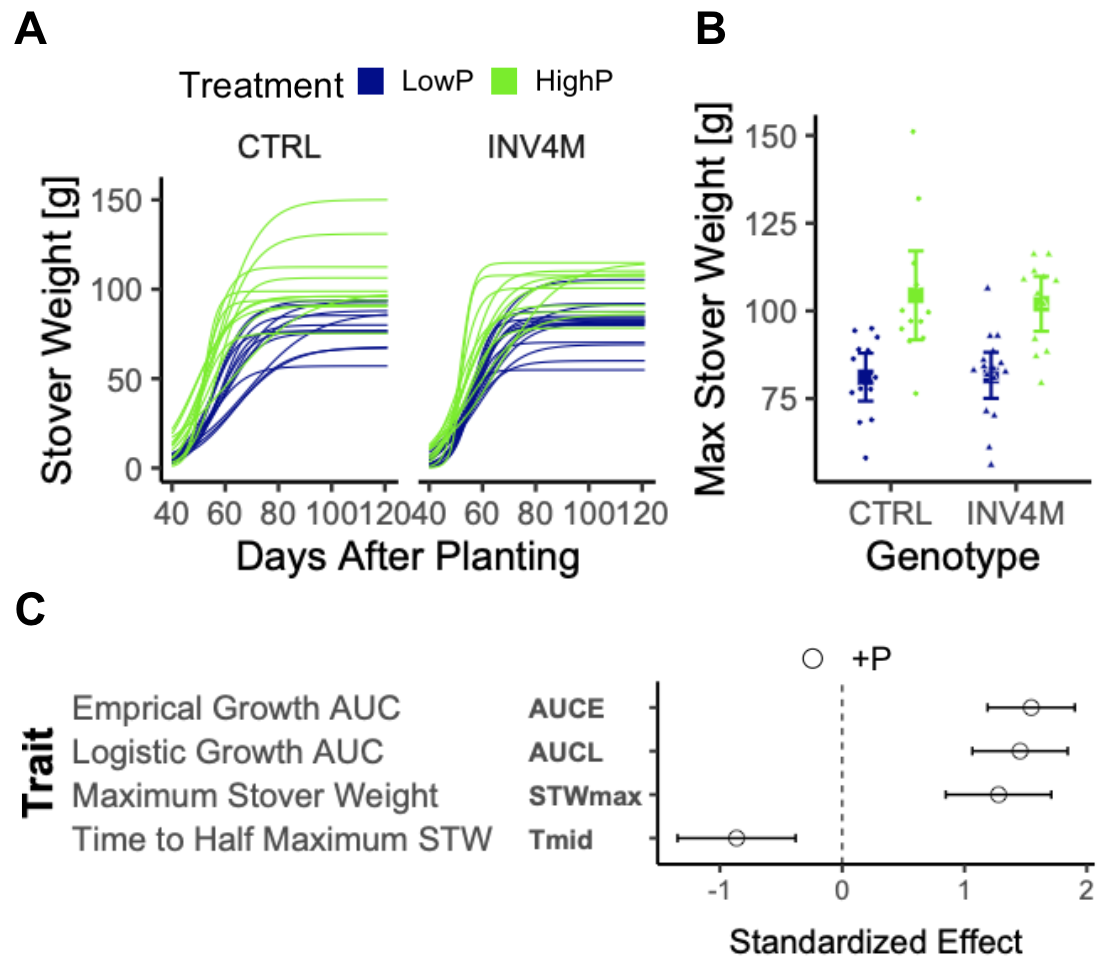
\includegraphics[width=\linewidth]{Chapter-3/figs/growth.png}
\caption[Plant growth curves show effect of phosphorus treatment but no \textit{\invfour} effect]{\textbf{\textit{Plant growth curves show effect of phosphorus treatment but no \textit{\invfour} effect.}}
% \\\hspace{\textwidth} 
\textbf{(A)} Stover dry weight, logistic growth fit curves per field row.
\textbf{(B)} Maximum Stover Weight mean and 95 percent confidence interval.
\textbf{(C)} Multivariable Multiple regression effect estimation mean $\pm$ 95 percent confidence interval (whiskers).
}
\label{fig::growth}
\end{figure}


\subsection{Leaf gene expression shows a marked response to Phosphorus and \invfour, with a single gene responding to \invfour $\times$ P interaction}

Plants showed a remarkable response to phosphorus in their leaf gene expression.
A multidimensional scaling analysis of the gene expression data (\autoref{fig::RNAseq} B) shows an overall response to phosphorus that tends to increase with more basal position of the leaf and is associated with the first dimension. 
The second dimension shows more separation between samples due to leaf position.

After a analysis for the effects of phosphorus treatment in gene expression we see that mir399 is consistently over-expressed from the most apical to the most basal of the sampled leaves.
Gene expression on target genes like SPX transporters was also consistently diminished in high phosphorus, corresponding to the overall expected response to phosphorus.

The phosphorus treatment has a genome-wise effect on gene expression, as shown by the mashr p-values {expression manhattan plots}. We found a total of 7373 differential expressed genes (out of  24249 genes detected in at least one leaf sample), with a distribution mostly consistent with gene density throughout the genome (\autoref{fig::RNAseq} C).
In contrast, the effect of \invfour is mostly detected inside the boundaries of \invfour 
% [I need to genotype the samples  show the actual boundaries  in these plants]
with a RNA-directed DNA polymerase, \textit{Zm00001eb190670} being the most significantly affected gene in the group.
Out of 528 DEGs detected for \invfour 263 genes that showed effect in cis, while 265 genes showed significant differential gene expression in trans between \invfour karyotypes.

% (mean fold value of the two groups, t-test p value (sperate hypothesis for over and under expressed genes?)).

\begin{figure}[!ht]
\centering
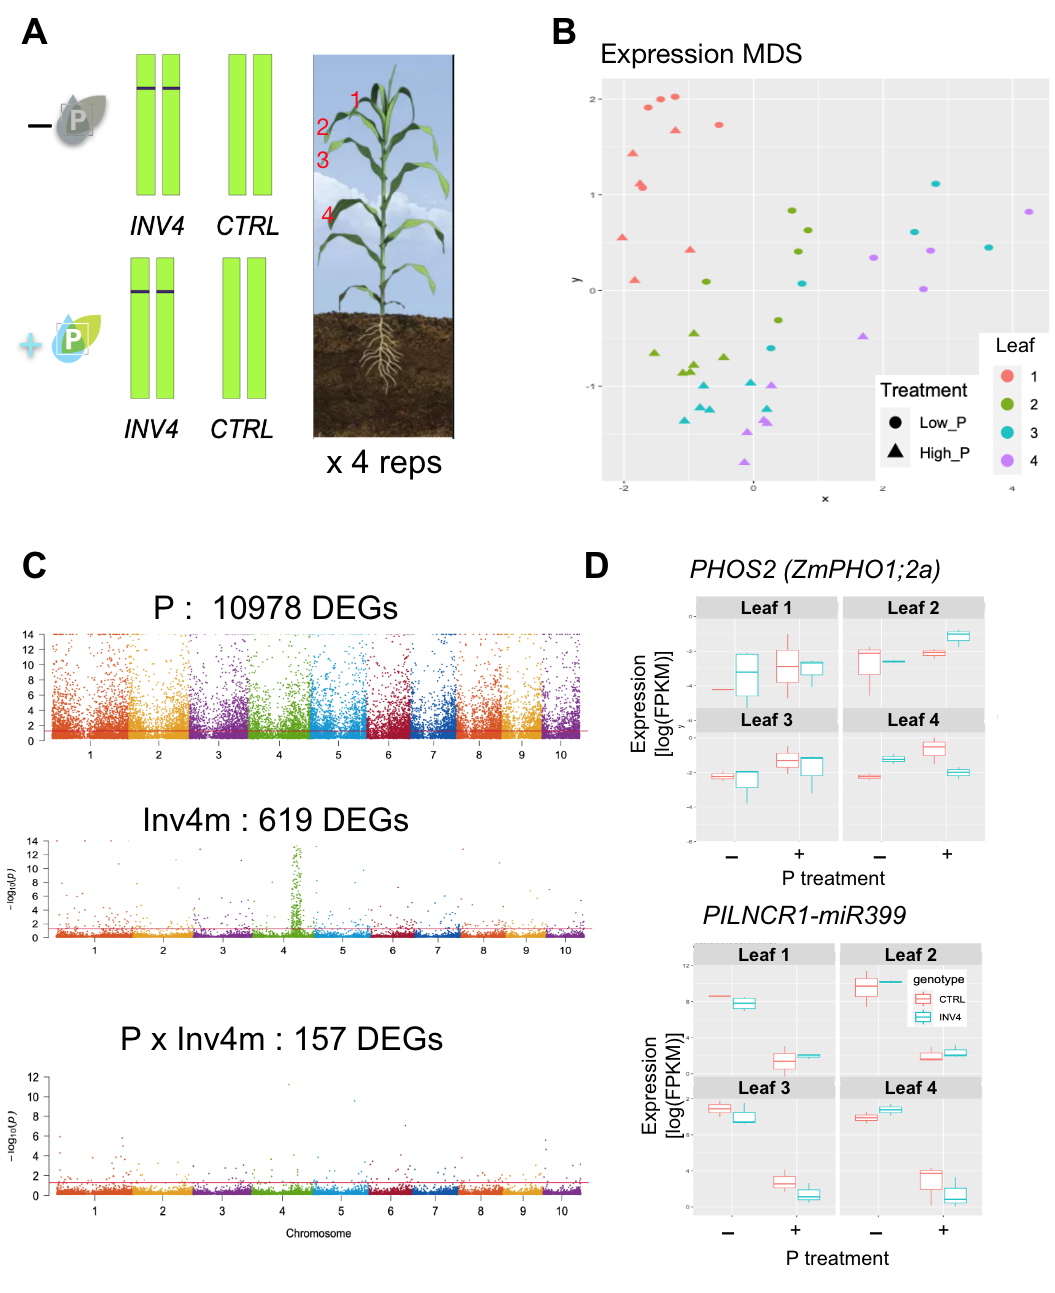
\includegraphics[width=0.95\linewidth]{Chapter-3/figs/RNAseq.png}
\caption[Effect of \invfour, Phosphorus Treatment and Interaction in Gene Expression]{\textit{\textbf{Effect of \invfour, Phosphorus Treatment and Interaction in Gene Expression.}}\\
\hspace{\textwidth} 
\textbf{(A)} Experimental Design.
\textbf{(B)} Gene Expression Multidimensional Scaling. Samples cluster by leaf and P treatment.
\textbf{(C)} Manhattan plots showing statistical significance of differential gene expression between P treatments, \textit{\invfour} genotype and P x \invfour interaction. Vertical lines in the inlay show the reported limits of \invfour \citep{calfee2021-mr}.
\textbf{(D)} \textit{top:} effect of P treatment on the PSR regulator \textit{PILNCR1-miR-399}, and \textit{bottom:} effect of the P x \invfour interaction on the expression of \textit{aldh2}.}
\label{fig::RNAseq}
\end{figure}
\clearpage

However, the variation at \invfour seems to have no major effectnn the gene response to phosphorus.
The \invfour x P interaction t-test (fdr <0.005) shows only one gene with differential response to phosphorus depending on the \invfour karyotype. This gene is found in  near \invfour, but outside previously reported limits (\autoref{fig::RNAseq} C).
A single gene \textit{aldh2}, 3 Mb upstream of the reported \invfour limit,  shows a different response  to phosphorus depending on the \invfour genotype. In phosphorus defficiency \textit{aldh2} overexpresses in  the CTRL plants, but it is not responsive in the \invfour plant (\autoref{fig::RNAseq} D).



\section{Discussion}

 The effect of \invfour in flowering time, previously reported as an association study hit \citep{romero_navarro2017-cn, barnes2022,gates2019-xu}, was confirmed by the experimental introgression of the isolated inverted haplotype into a single genetic background (B73). 
 Additionally, we observed that in this particular background \invfour, increases plant height at flowering.
 These two effects are additive with the corresponding effects of phosphorous treatment. 
 The response of the experimental plants to phosphorus was observed in more phenotypes and was of greater magnitude than the effect of \invfour (\autoref{fig::effects}). 
 In phosphorus deficiency the plants showed delayed growth as both a later time to half maximum stover dry weight and longer times to male and female flowering.
 Plants grew smaller in the absence of phosphorus, accumulated less vegetative biomass as stover dry weight at harvest, and had smaller kernels (KW50) (\autoref{fig::effects}).
 No significant \invfour $\times$ P interaction was detected ($\beta$ t-test, $\textrm{fdr} > 0.05$ for all phenotypes).
 Regarding leaf transcriptome, the master regulator of the phosphorus starvation response  \textit{PILNCR1-mir399} was over-expressed in phosphorus deficiency independent of \invfour genotype (\autoref{fig::RNAseq} D). 
 \textit{PILNCR1-mir399} has been reported to be overexpressed in low phosphorus, and in particular it is more responsive in P-inefficient than in P-efficient genotypes \citep{du2018}.
 B73 has been reported to be phosphorus inefficient with respect other inbreds like Mo17\citep{zhu2005}, and has been selected for yield under high input agriculture compared with traditional varieties such as Mi21. However, \textit{PILNCR1-mir399} response to phosphorus in the experimental plants show no dependency on the variation at \invfour. 
 This suggests that the master regulator phosphorus starvation response is not regulated by \invfour in the experimental conditions. 
 An alternative explanation, is that the experimental P limitation was not hard enough to show a genotype-dependent difference in response. 
 No observable difference in anthocyanin accumulation, or lower leaf senescence in response to phosphorus deficiency in the plant leaves was observed in the field.

We observed a clear over-representation of nitrogen-associated biological processes and metabolic pathways in the 7373 genes responsive to phosphorus treatment (Fisher exact test GO over representation adjusted FDR < 1e-6). 
However, when we reduce the list to the top 1000 most significant, the over-represented gene processes and terms are more related to phosphorus (Fisher exact test GO over representation adjusted FDR < 1e-6). 
This suggests that the genes that show the greater and/or more consistent effect  have phosphorus-associated functions while nitrogen-related genes are making significant but smaller adjustments in expression, maybe reflecting cross-talk between phosphorus and nitrogen homeostasis\citep{torres-rodriguez2021}.
I could not find signals of photosynthesis or carbohydrate over representation in the \invfour responsive to inversion karyotype, as was previously found in response to cold \citep{crow2020}.
 
Overall, there is no evidence from this transcriptome experiment that \invfour contributes to local adaptation to phosphorus, in the sense that its adaptive contribution does not depend on phosphorus amount in the the soil.
However, it is clear that \invfour plants flower earlier and are taller irrespective of the phosphorus status.

\newpage

\printbibliography[heading=subbibnumbered, title=References]


\chapter{Ionomics of the Andosol Introgression Resource Panel: Kernel Nutrient Accumulation and Potential Adaptations to Highland and Lowland Phosphorus Deficiencies}
\label{chap-three}

\newrefsection

\section{Background}
Andosols are soils of volcanic origin that support maize crops, pasture grasses, and native forests in the highlands of Mexico \citep{bayuelo-jimenez2020,galvan-tejada2014}. Maize has been cultivated in the Mexican Highlands for the last 6500 years \citep{piperno2001} without industrial fertilizers.
Adaptation to low phosphorus availability is evidenced by local corn varieties that, have increased phosphorus use and acquisition efficiency when grown in the Andosols of the highland plateau of the Transmexican Volcanic Belt (TMVB) \citep{bayuelo-jimenez2011,bayuelo-jimenez2014} \ref{fig::parentmap}.

\begin{figure}[!ht]
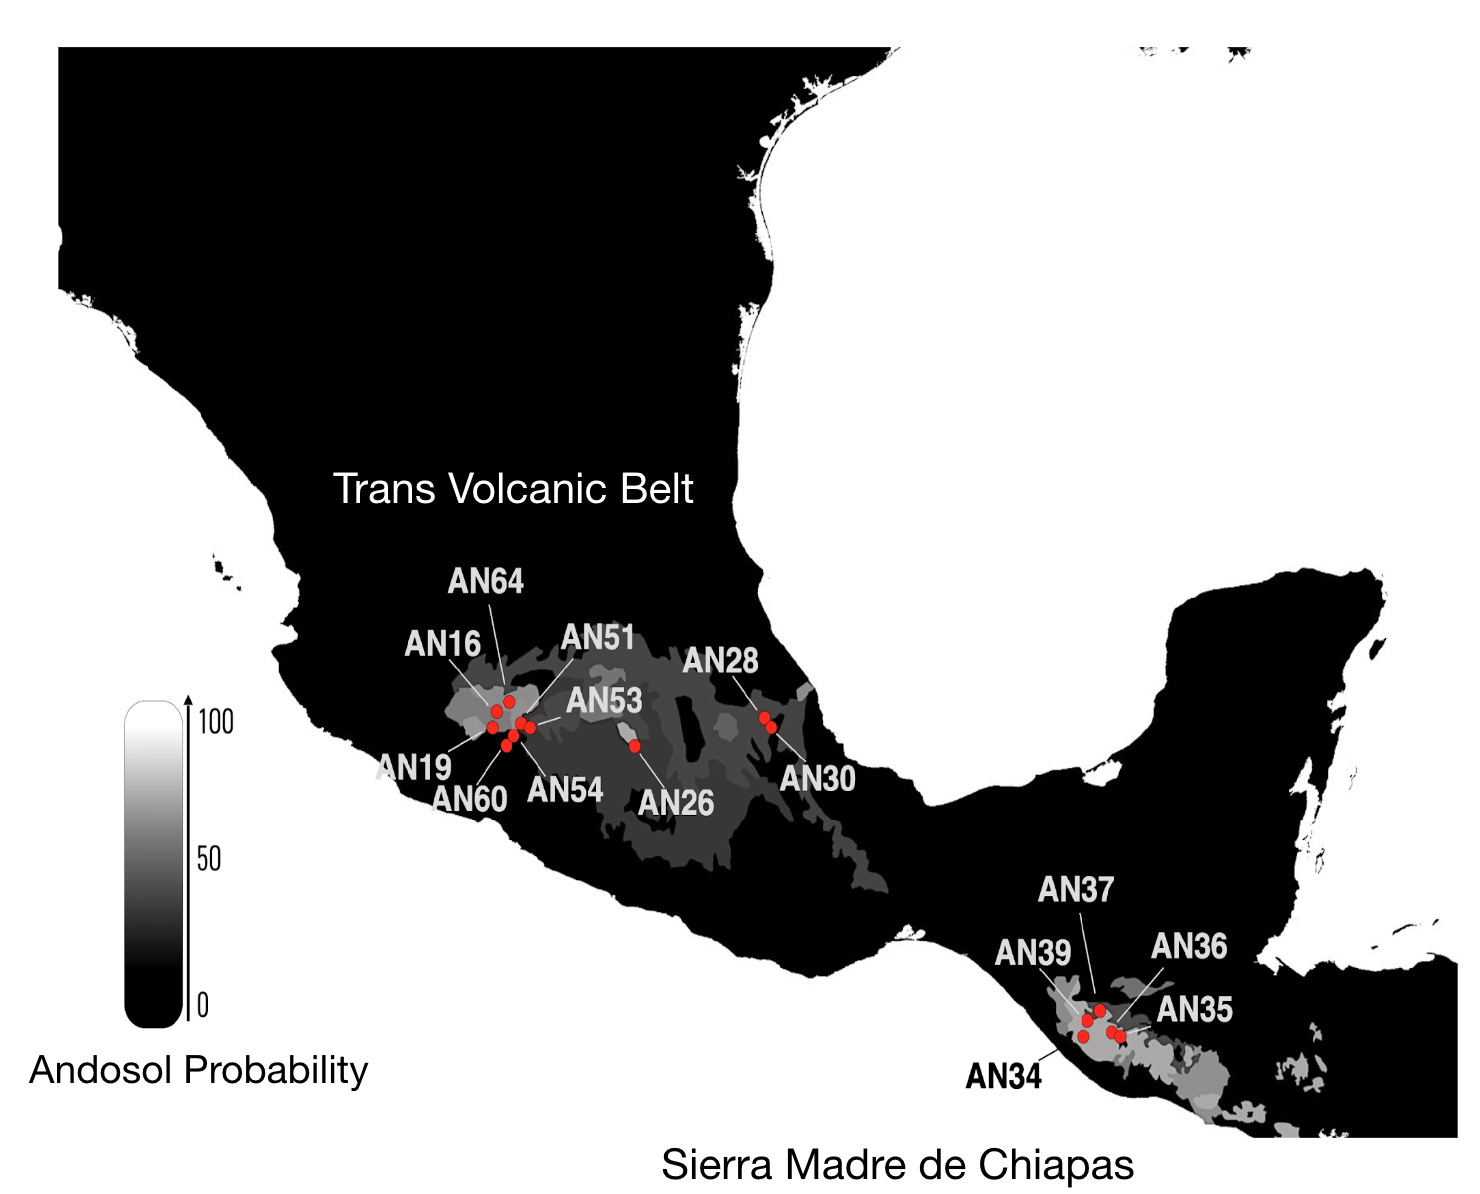
\includegraphics[width=\linewidth]{Chapter-4/figs/parentmap.png}
\caption[ Geographic Distribution of AIR Panel Andosol Founders]
\textit{{\textbf{Geographic Distribution of AIR Panel Andosol Founders }}
15 landraces were selected from Mexico and Guatemala Andosols to be founders of the populations}
\label{fig::parentmap}
\end{figure}

In this work, we use ionomics to search for quantitative trait loci for kernel mineral content, including phosphorus, in a segregating population as a step to understand the genetic basis of kernel mineral composition underlying nutrient use efficiency.
Our maize mapping population has been derived from 15 founder landraces native to the Mexican Andosols, crossed to CML530, a tropical inbred selected for adaptation to acid soils in Colombia \citep{granados1995}.
These crosses might combine different phosphorus use efficiency strategies in maize, the donor landraces conferring adaptation to highland andosols, and the recurrent parent, CML530, adaptation to the acidic ferralsols of the Andean piedmont.

\subsubsection{Nutrient Restrictions in Andosols}

Because of their tendency to retain phosphates, Andosols productivity is limited by the amount of soluble phosphorus they have available for plant intake. Volcanic glass is the source of the Andosols’ high content of alumino-silicate and ferrihydrites that transform over time into allophanes and imogolites \citep{wrb2022}
These minerals make Andosols highly acidic soils and confer them a high cation exchange capacity, due to both, their high surface area and large number of reactive sites.
In these acidic conditions, aluminum and iron cations promote complexes that precipitate phosphates out of the soil solution and strongly bind them to the soil particles \citep{krasilnikov2013}. Plnat adaptations that allow extraction of these occluded minerals might increase the acquisition of phosphorus from a difficult source.

\subsubsection{Genes controlling ionomics in the maize kernel}

Single-kernel ionomics is a valuable approximation for investigating the genetic basis of nutrient  assimilation in corn.
Mineral content in single kernels show enough heritability to be amenable to genetic analysis in the search for candidate loci \citep{baxter2014,baxter2013}. 

\section{Methods}

\subsection{AIR: Andosol Introgression Resource. A novel maize mapping population for the genetic characterization of maize adaptation to low phosphorus availability.} 

We have developed a unique collection of Near Isogenic Lines (NILs) by crossing 15 Mexican highland landrace accessions to the elite CIMMYT inbred background CML530.
The landrace donors used can be divided into two large groups. The first group of 10 landraces represents the Trans-Mexican Volcanic Belt (TMVB) that crosses Mexíco from West to East.
Landraces from TMVB were selected mainly from the Purepecha plateau of Michoacan, in the locality of the Cerro de Tancítaro/Parícutin volcano, a region documented to harbor highly phosphorus-efficient maize \citep{bayuelo-jimenez2011}. The other donors from this group were selected from the Estado de Mexico (Nevado de Toluca volcano) and Veracruz (Cofre de Perote volcano).
All donors from this group were highland sourced, ranging from 1902m to 3017m above sea level, representing seven primary landraces (Table 1). The second group of landraces was sourced from the Andosols of the Sierra Madre de Chiapas (SMC), representing a demographically distinct group of landraces from a different mountain range. This group represents high and lowland landraces, including accessions from Olotón. This landrace has been shown to exude mucilage associated with the recruitment of nitrogen-fixing bacteria \citep{vandeynze2018}.
We backcrossed (BC) each donor twice into the CIMMYT CML530 background - an elite acid soil tolerant line developed from the synthetic population SA-8 \citep{granados1995} - before selfing (S) for three generations. We have produced 1372 BC$_2$F$_3$ families.
A single F1 individual was used for each of our 15 individual populations, capturing a single haplotype from each outbred donor, ensuring each population was biallelic. Each family contains 12.5\% landrace genome in the CML530 background. During the Winter nursery of 2020-21 in Puerto Vallarta, we planted 18 seeds of the BC$_2$F$_3$ ears, and plants within the row were sib-mated and bulked to generate seed for future experiments. On average, we generated ~ 1 kg of seed for each of the 1372 families.
This type of population (BC$_2$F$_3$) has been highly successful in the identification of several types of traits involved in maize domestication \citep{xu2017b,guo2018a,liang2019,tian2019}.


\begin{figure}[!ht]
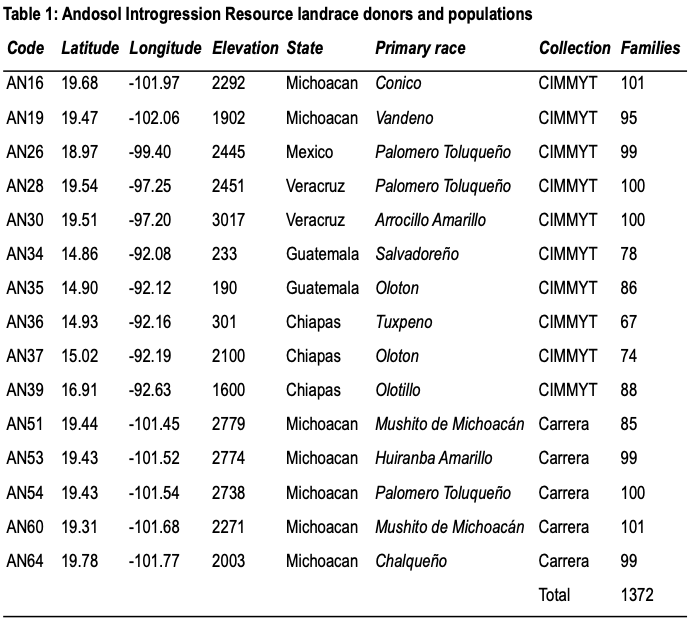
\includegraphics[width=\linewidth]{Chapter-4/figs/parentdata.png}
\caption[AIR Founders Passport Information]{ \textit{{\textbf{AIR Founders Passport Information}}}}
\label{fig::parentdata}
\end{figure}


\begin{figure}[!ht]
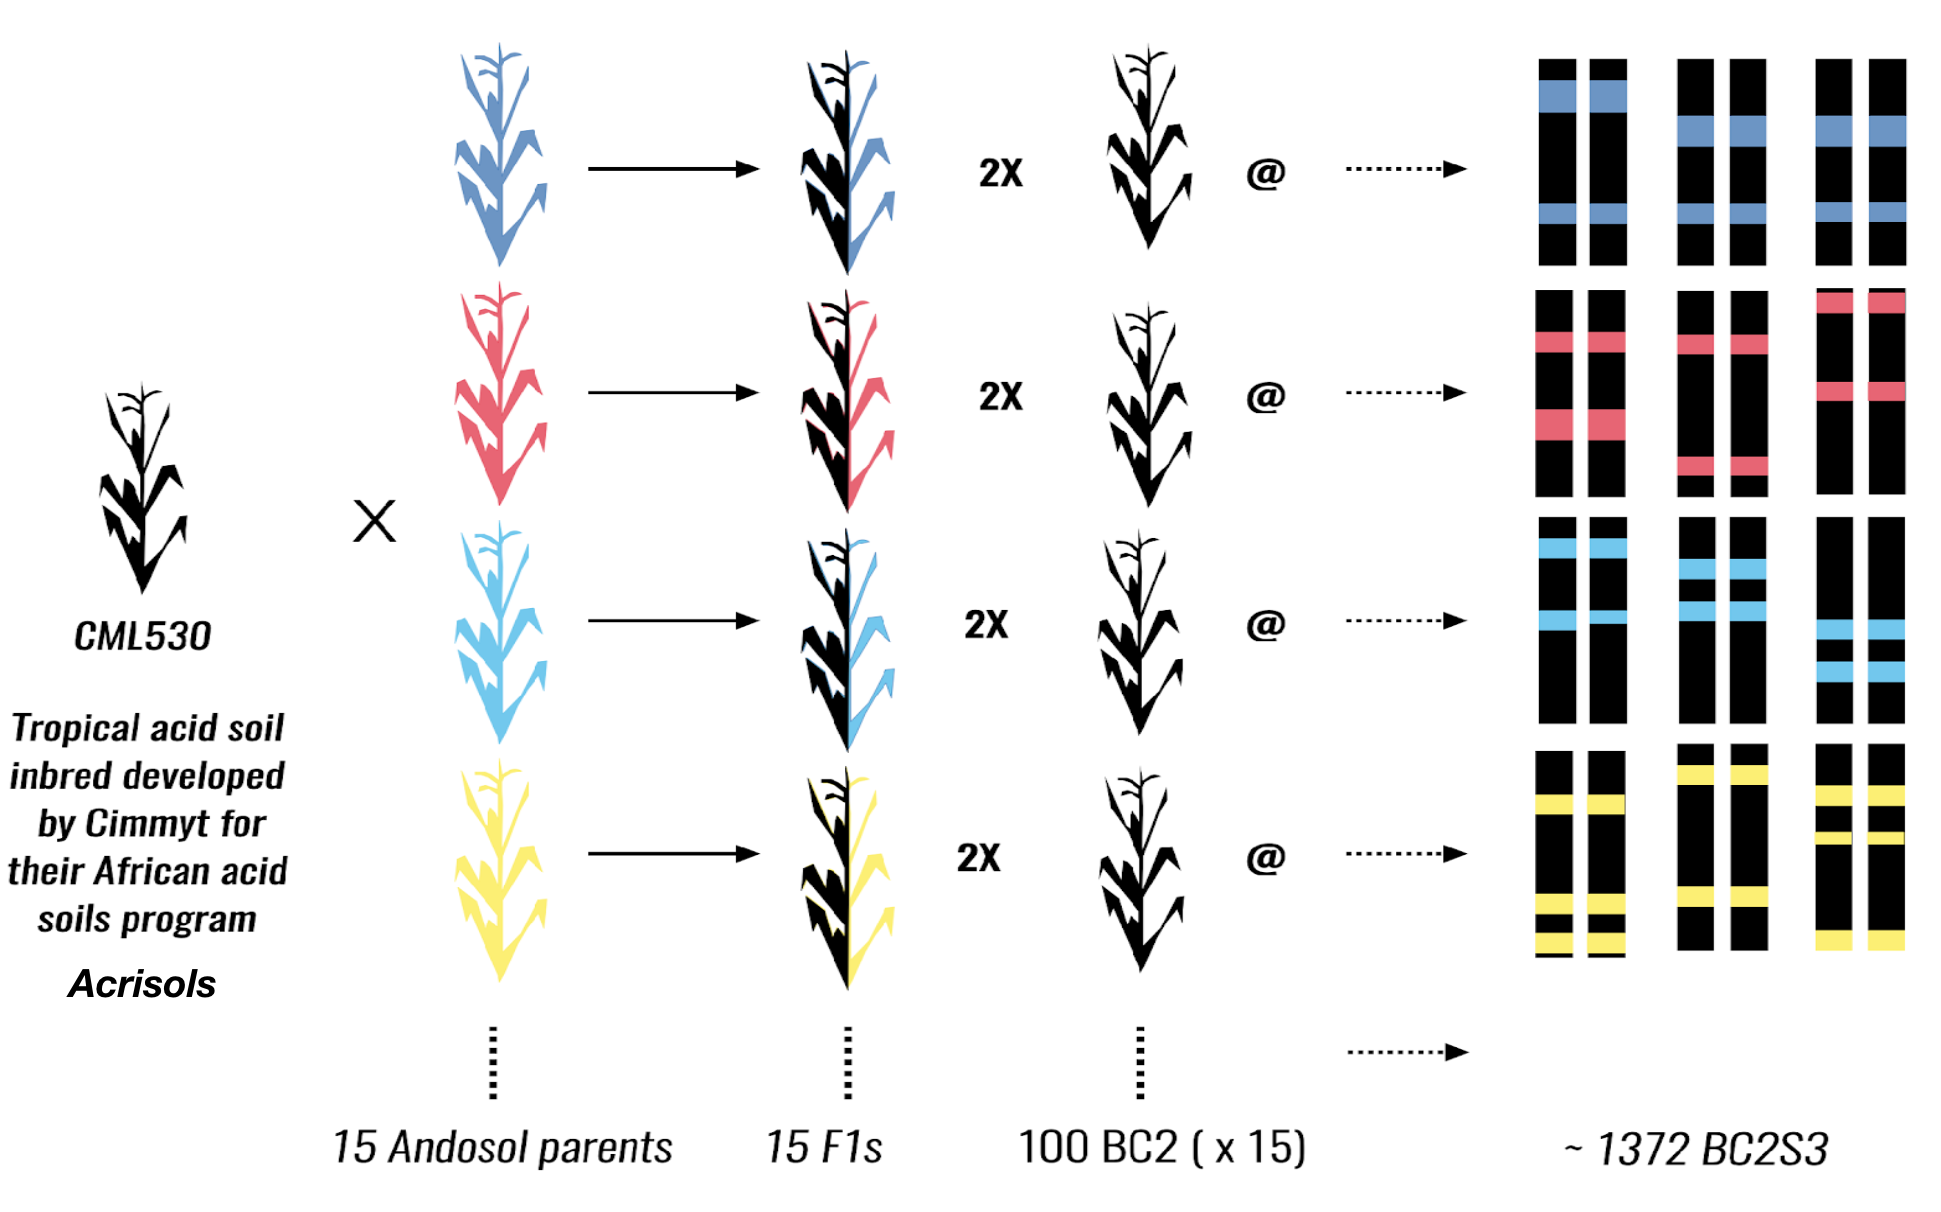
\includegraphics[width=\linewidth]{Chapter-4/figs/AIR_design.png}
\caption[ AIR Panel (Andosol Introgression Resource) Breeding scheme]
{\textit{{\textbf{AIR Panel (Andosol Introgression Resource) Breeding scheme}}}
15 landraces were selected from Mexico and Guatemala Andosols to be founders of the populations}
\label{fig::airdesign}
\end{figure}


\subsection{Genotyping}
 To genotype the BC$_2$F$_3$ families, we first sequenced the 15 F1 CML530 x landrace founder individuals and the CML530 recurrent parent using Illumina, generating an average of 30x coverage. In total, we generated ~ 85 million SNPs.
 We identified ~101,000 thousand SNPs that were common across all F1 individuals and were heterozygous between the landrace parents and CML530. From this set of SNPs, we used plink's LD Pruning tool to select a subset of SNPs unlikely to be in linkage disequilibrium. Using a window size of 50kb and selecting 5 SNPs per window,  we obtained a final set of ~ 3,000 SNPs.
 We then designed primers for amplicon sequencing using LGC Seq-SNP technology. This technology involves the design of primers flanking SNPs of interest.
 We then designed primers for amplicon sequencing using LGC Seq-SNP technology.
 This technology involves the design of primers flanking SNPs of interest.
 After PCR amplification, samples are sequenced via Illumina. We obtained good amplification of around 2500 markers distributed throughout the genome, sufficient to build and saturate a genetic map using R/QTL \citep{broman2012}

\subsection{ICPMS}.
We selected a representative kernel from each AIR line seed bulk and processed it for ICPMS.
The final concentrations of minerals were calculated as mg of element per kg dry seed weight. We checked for clustering of the ionomics profile regarding andosol donors and mountain range source using a PCA analysis of the mineral content.

\subsection{QTL Mapping}
We used single marker QTL mapping in BC$_2$F$_3$ population according to R/QTL manual \citep{broman2012},  making associations for the 14 traits.  We established the statistical threshold after 10000 permutations of the phenotype with respect to genotypes.  We did both, joint analysis with the whole population data and analysis per donor family.
The joint analysis increases our power to detect signals from similar allelic effects coming from different Andosol donor backgrounds.
And the separate family analysis allows us to detect QTLs unique in each family at the cost of reduced power. To test the quality of and the potential of  our map for mapping phenotypes related to  Andosols, we decided to make  a QTL analysis of two other phenotypes that have presumptive adaptive roles in maize heirlooms to the highlands of Mexico.
We scored both stem macro hairs and  the presence of anthocyanin pigments in stems as binary (presence/absence) traits. 


\section{Results}
\subsection{Ionome diversity}
The minerals quantified by ICPMS have two types of distributions. The most abundant ions (median x-y ppm) including Potassium, Sulfur and Phosphorus, tend to have more symmetrical and approximately normal distributions, while the less abundant ions (median x-y ppm) have a  heavily right-skewed distribution, like boron, nickel and aluminum.
Skewed data might better be log-transformed for linkage mapping purposes, as the associations might be linear with the order of magnitude rather than the untransformed concentration in the kernel. As a matter of fact The first two principal components of a naive PCA on the untransforme data show a separation of contributions according to the type of distribution.
Skewed data minerals,Al, B, Mo, Ni, (Jarque-Bera test FDR <0.05 table, ions sorted by median abundance, with skewdness and kurtosis measurements) have mayor contributions to the second principal component (12.1 \% variance) while the more abundant and symmetrically distributed ions make the bulk of the contributions to the first principal component.
A PCA on log-transformed low abundance minerals might reveal a different variance-covariance structure where the log(abundance) might vary less orthogonally to other minerals. A hierarchical clustering of the minerals on the untransformed space shows again, a tight clustering of the rare long tail distribution minerals, and les well-defined clusters corresponding to mostly bivalent cations and iron, Fe,Mg,Mn,Zn, with P,S,K, with other correlated pairs being Na,K and surprisingly Aluminum and calcium . This correlation structure must reflect two underlying causes.
First, the similar chemistry and biological functions of the minerals in the plant tissues. And second, their correlated abundance and bioavailability in the soil.
\clearpage

\begin{figure}[!ht]
\begin{center}
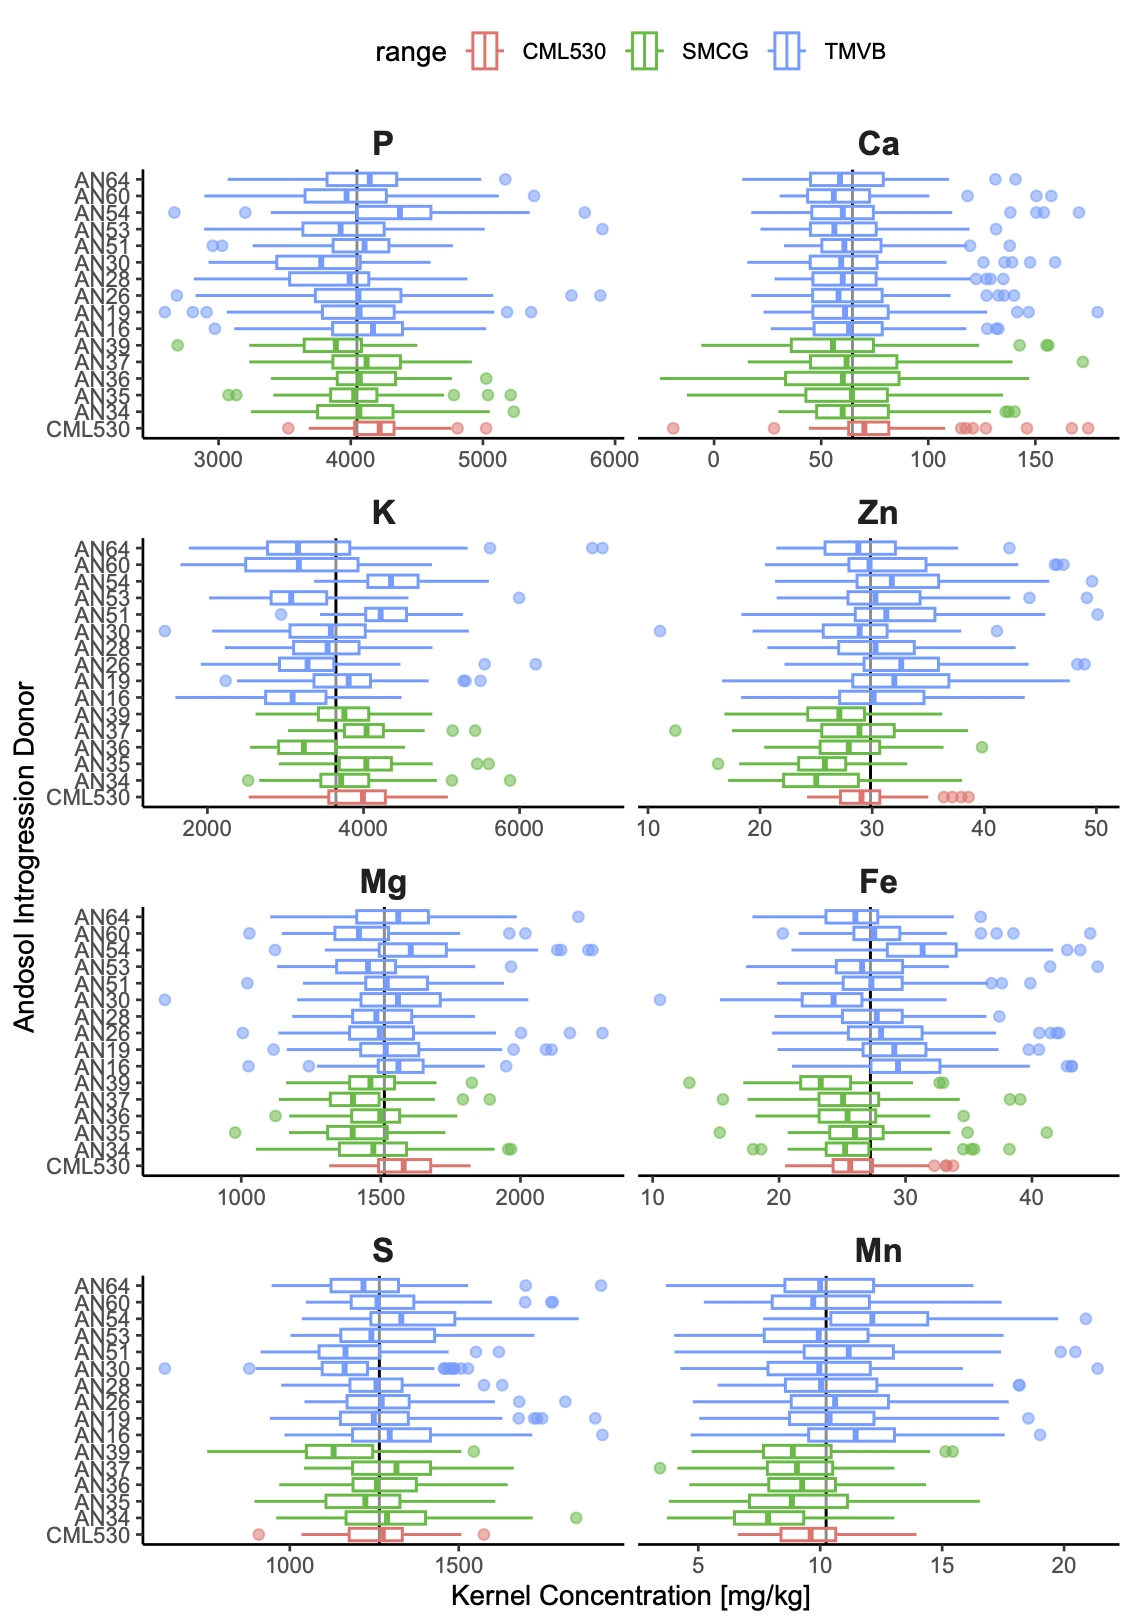
\includegraphics[width=0.8\textwidth]{Chapter-4/figs/mineral_distro.png}
\caption[Distribution of mineral kernel concentration]\textit{{\textbf{Distribution of mineral kernel concentration}} Minerals sorted by mean abundance from top to bottom, boxes with median, IQ range, whiskers $95\%$ quantiles. Families derived from Sierra Madre de Chiapas y Guatemala (SMCG, n=375), have a distinct mineral content (MANOVA, p<1e-12) than either Transmexican Volcanic Belt (TMBV, n=910, Zn, Mg, Fe, Mn), or CML530 material (n=70, Mg, Zn, Mn).}
\end{center}
\label{fig:mineraldistro}
\end{figure}
\clearpage

\begin{figure}[!ht]
\begin{centering}
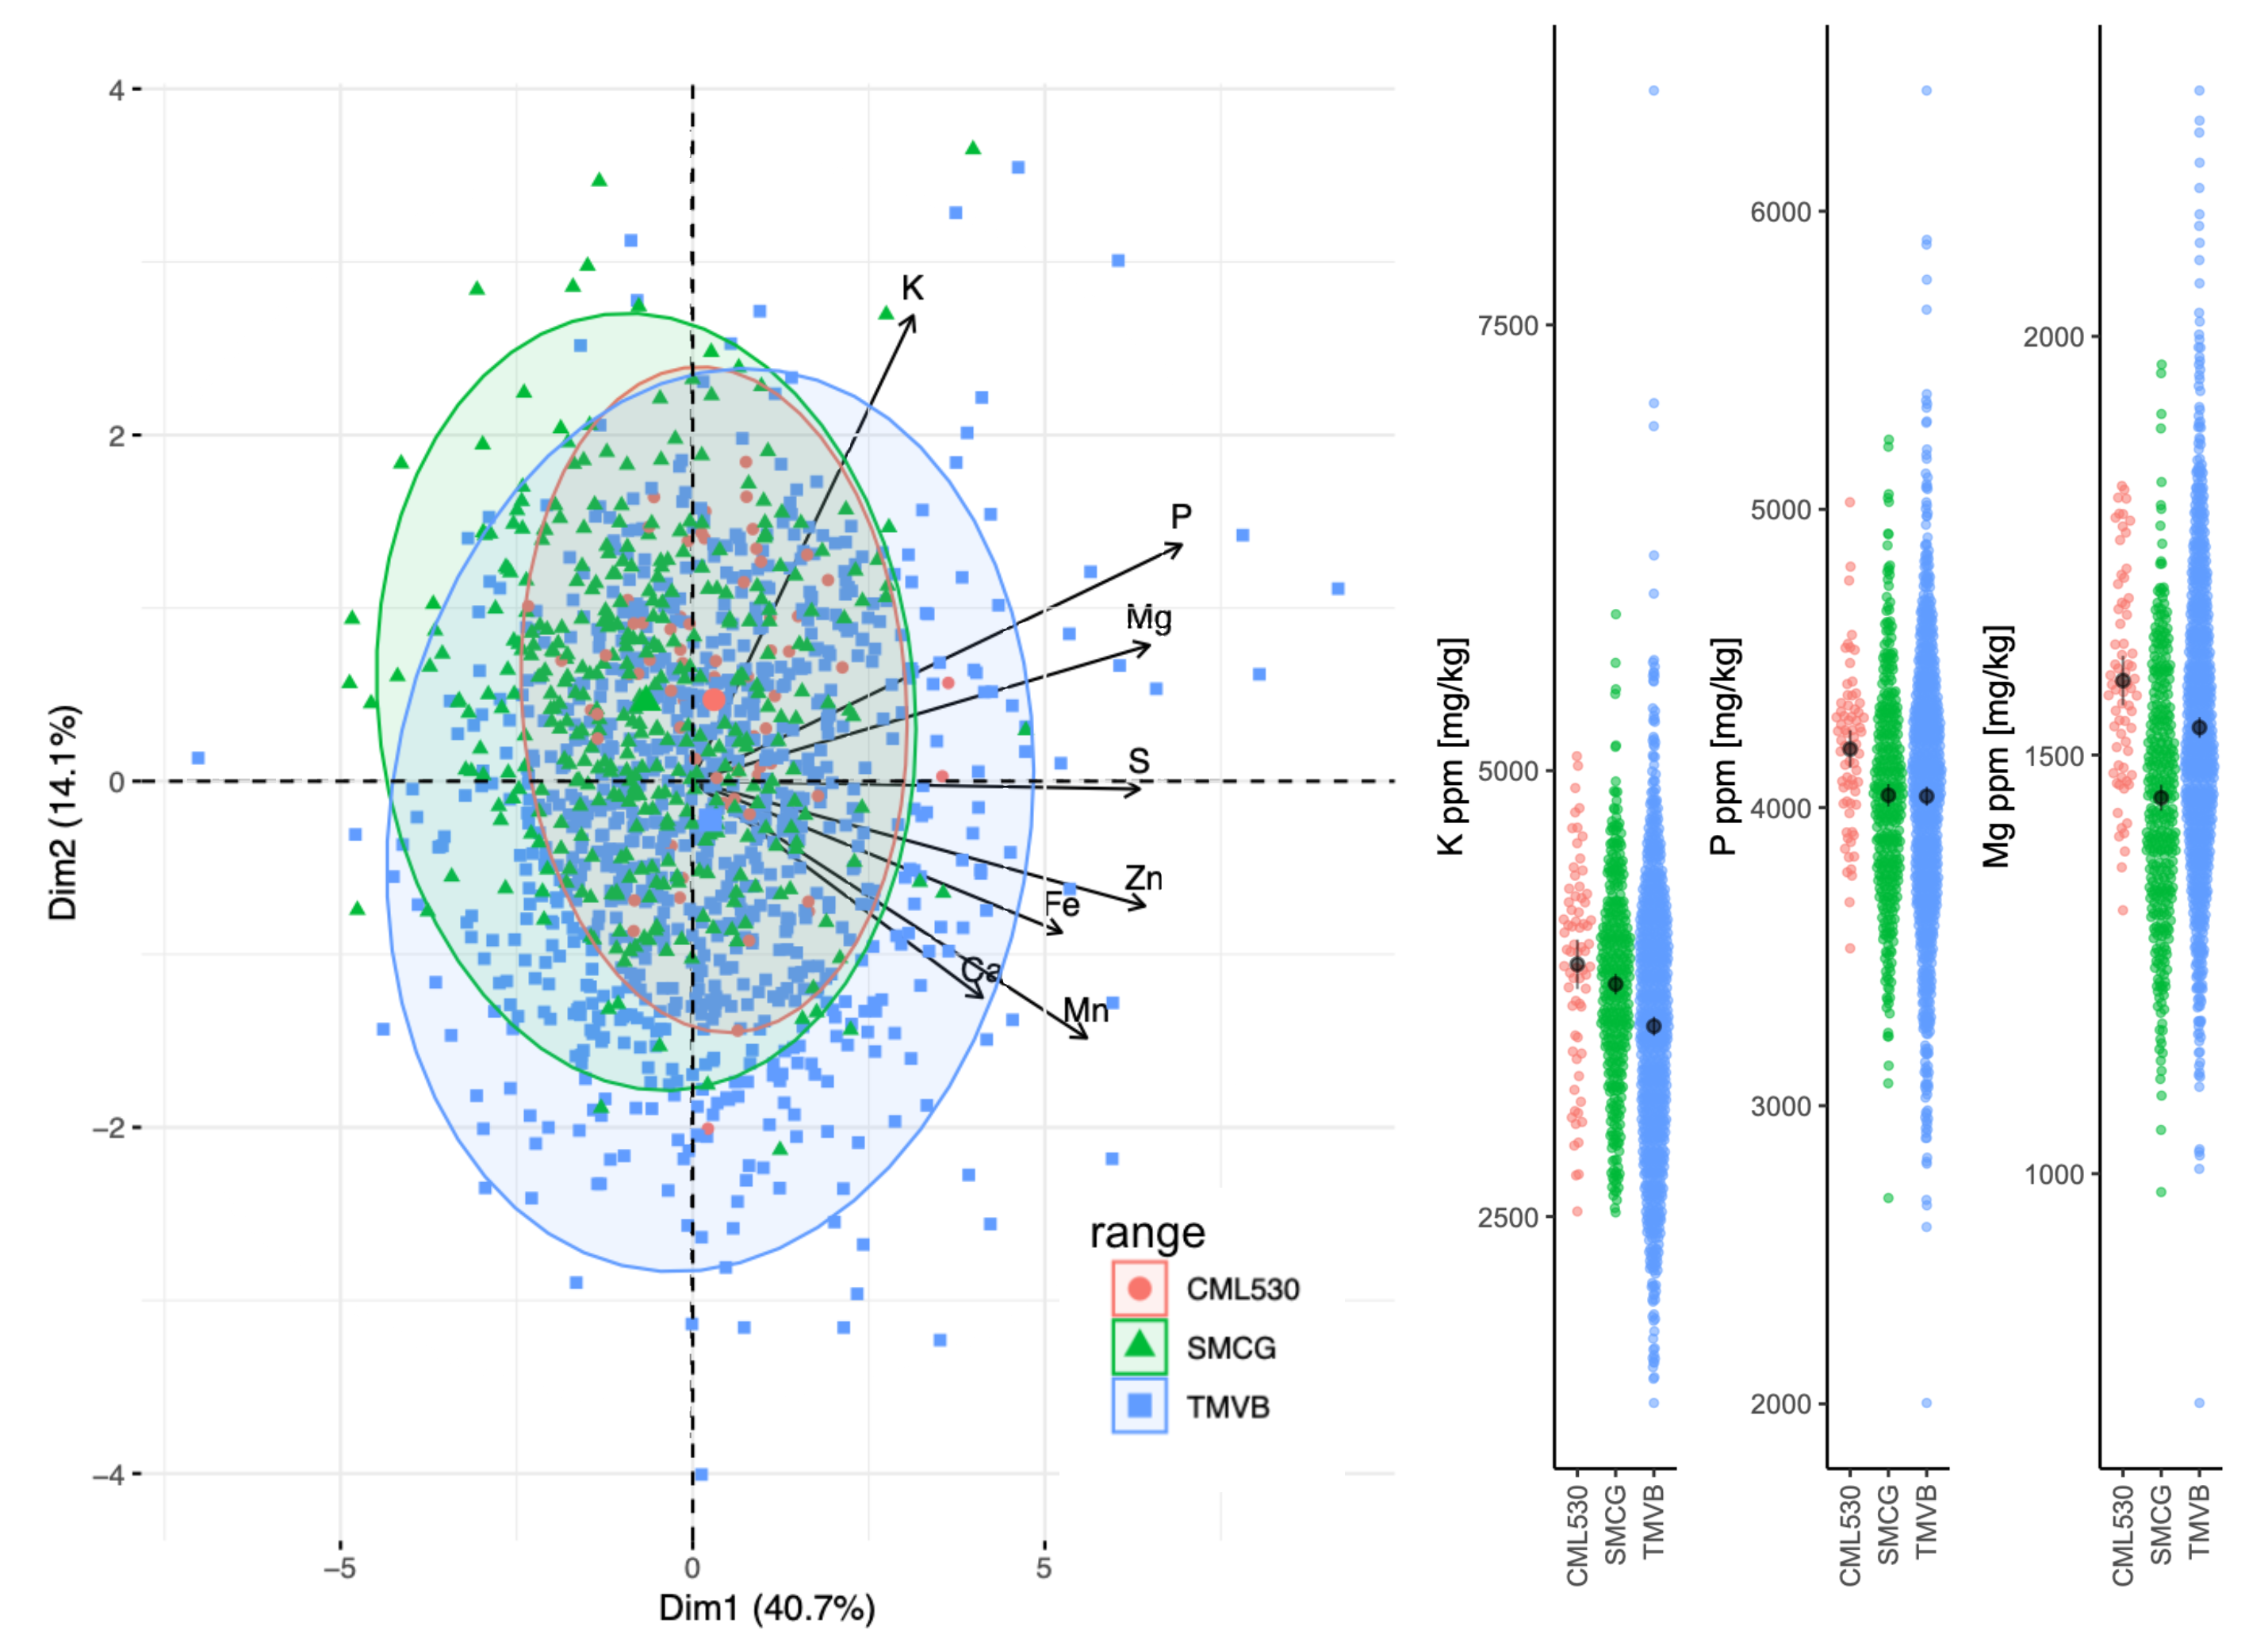
\includegraphics[width=\textwidth]{Chapter-4/figs/mineral_PCA.png}
\caption[Kernel Mineral PCA]{\textit{\textbf{Kernel Mineral PCA}}. \textit{Left:} First dimension has a high contribution from P, Mg, Zn and S; the second dimension's main contribution is from K.  \textit{Right:} there are significant differences between the mineral composition of families derived from parents of different geographic range (SMCG and TMVB) and the recurrent parent CML530.}
\end{centering}
\label{mineralPCA}
\end{figure}
\clearpage

\subsection{Linkage Map.}
The genetic PCA showed evidence of genetic outliers that most likely are due to contamination.Thus we calculated kinship coefficients (manichakul etal) and discarded x outliers.
We obtained a joint genetic map with 2300 markes of 2500 cM, with mean distance of 1 Mb/cM and sd dev of 1 Mb/cM, no gap grater than 10 cM, in good agreement with our expectations from marker design (mean 1Mb/cM, sd = 1Mb/cM).
Our genotype table has a completenes of 95\%, with mean 95 ccompleteness per marker and 80 ccompletness per individual.
We found a predictable excess of heterozygous given that samples were pooled per row and the genotype calling software penalyzes the homozygote calls.  We found low recombination rates around the reported centromeres (mean sd, t test).
Genetic Maps per individual family varied, as  many alleles were not  polymorphic, and thus excluded, in certain families do to lineage sorting.



\begin{figure}[!ht]
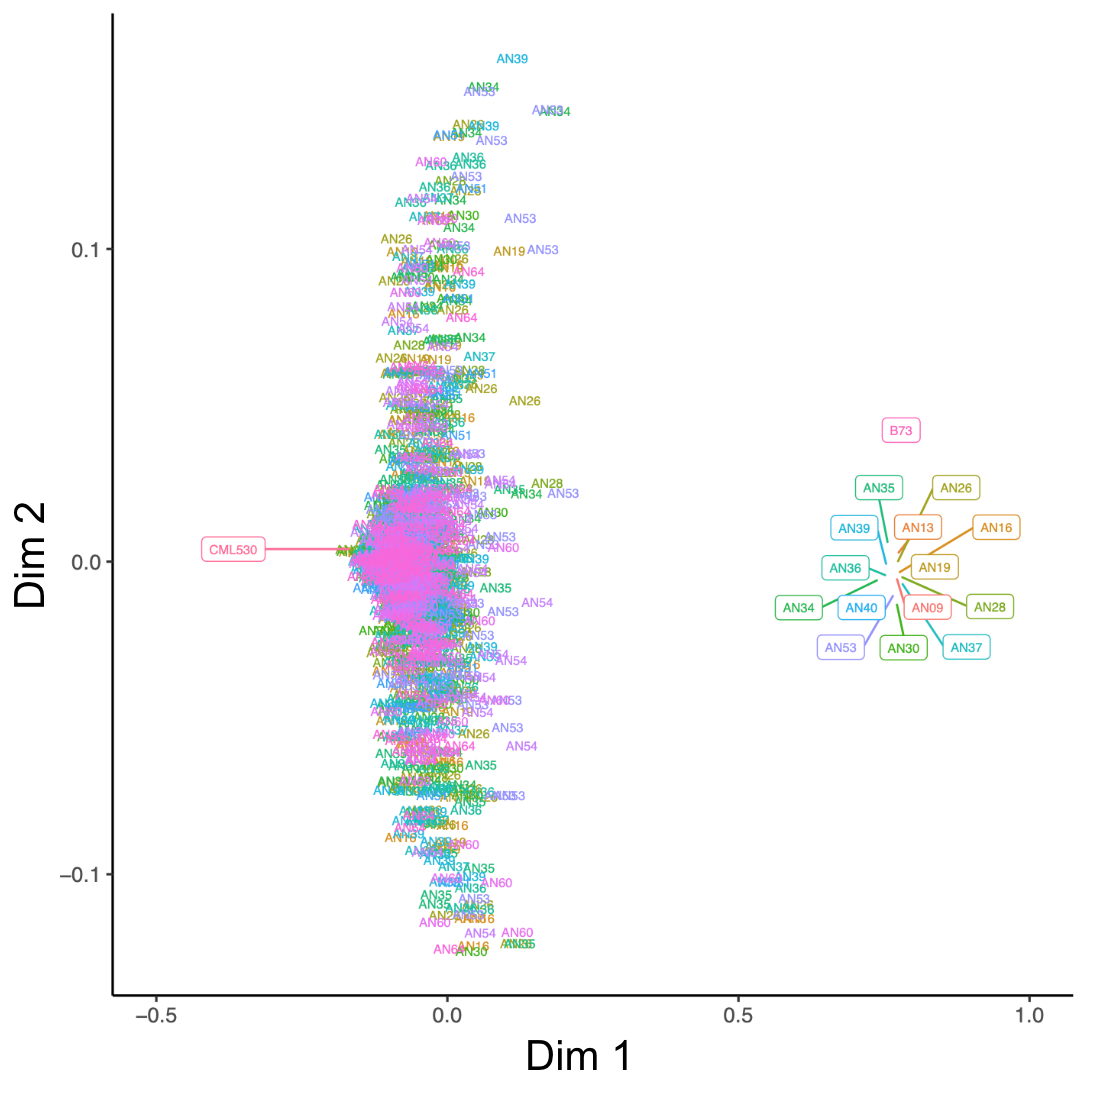
\includegraphics[width=0.8\paperwidth]{Chapter-4/figs/genetic_MDS.png}
\caption[Genetic PCA of AIR lines]{\textit{\textbf{Genetic PCA of AIR lines.}}
Dim1 has an enormous contribution to genetic variance, and it is not correlated with either donor or geographical origin. Possible contaminations can be seen in kinship distribution}

\label{Fig3.3}
\end{figure}
\clearpage


\begin{figure}[!ht]
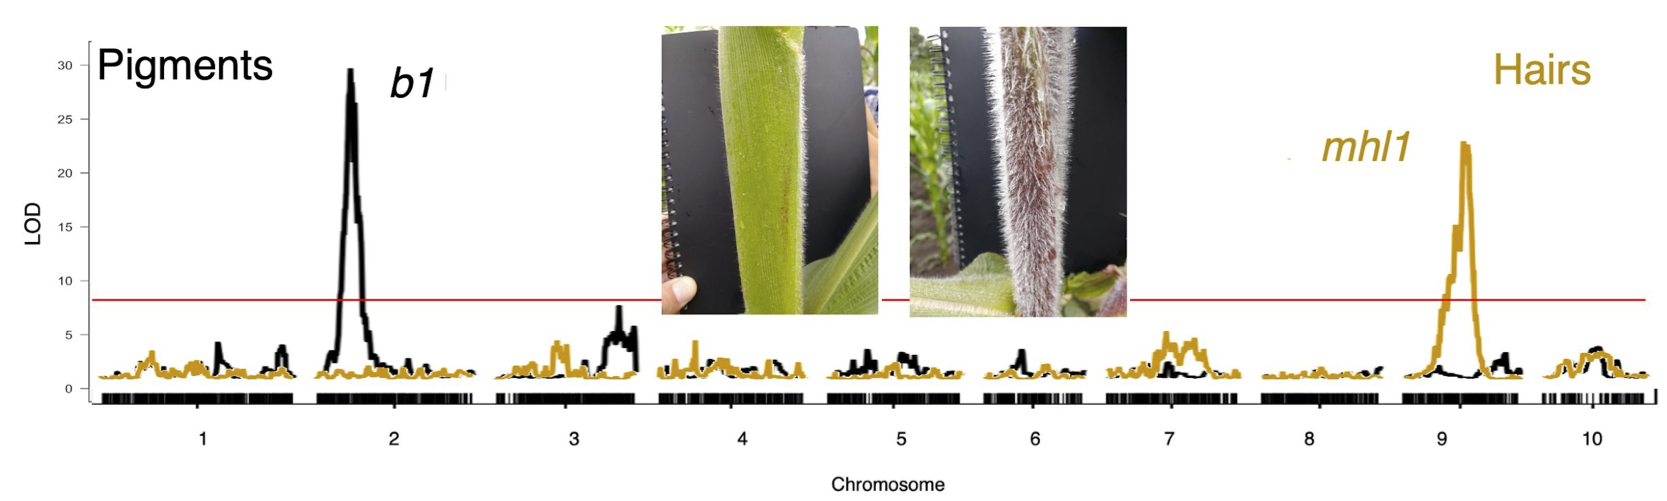
\includegraphics[width=0.8\paperwidth]{Chapter-4/figs/highland_traits.png}
\caption[QTL mapping for presumptive Highland Adaptive traits]{\textit{\textbf{QTL Mapping for presumptive Highland Adaptive traits}} Strong signals were detected for both macro hairs and anthocyanin pigmentation coinciding with previously reported loci \textit{b1} and  \textit{mhl1}.
}
\label{fig:highlandtraits}
\end{figure}


\subsection{QTL Mapping.}
As a quality check we were able to locate strong and highly significant QTLs for stem macro-hairs (LOD =15), and anthocyanin pigments (LOD =20), and colocalized with previously reported loci R1 an mhl1.

In the joint map we found genome wide significant single marker QTLs for all minerals measured as described in figure 3. The most significant hits were found for Mn, Mg and Ni.  Of our particular interest Phosphorus showed a robust QTL in chromosome 8.

% QTLs that were found in the joint analysis but not in the per family analysis

% Family specific QTLs.

% QTLs  showing matching  effect sign through families

% QTL showing incongroun signs between familes


\begin{figure}[!ht]
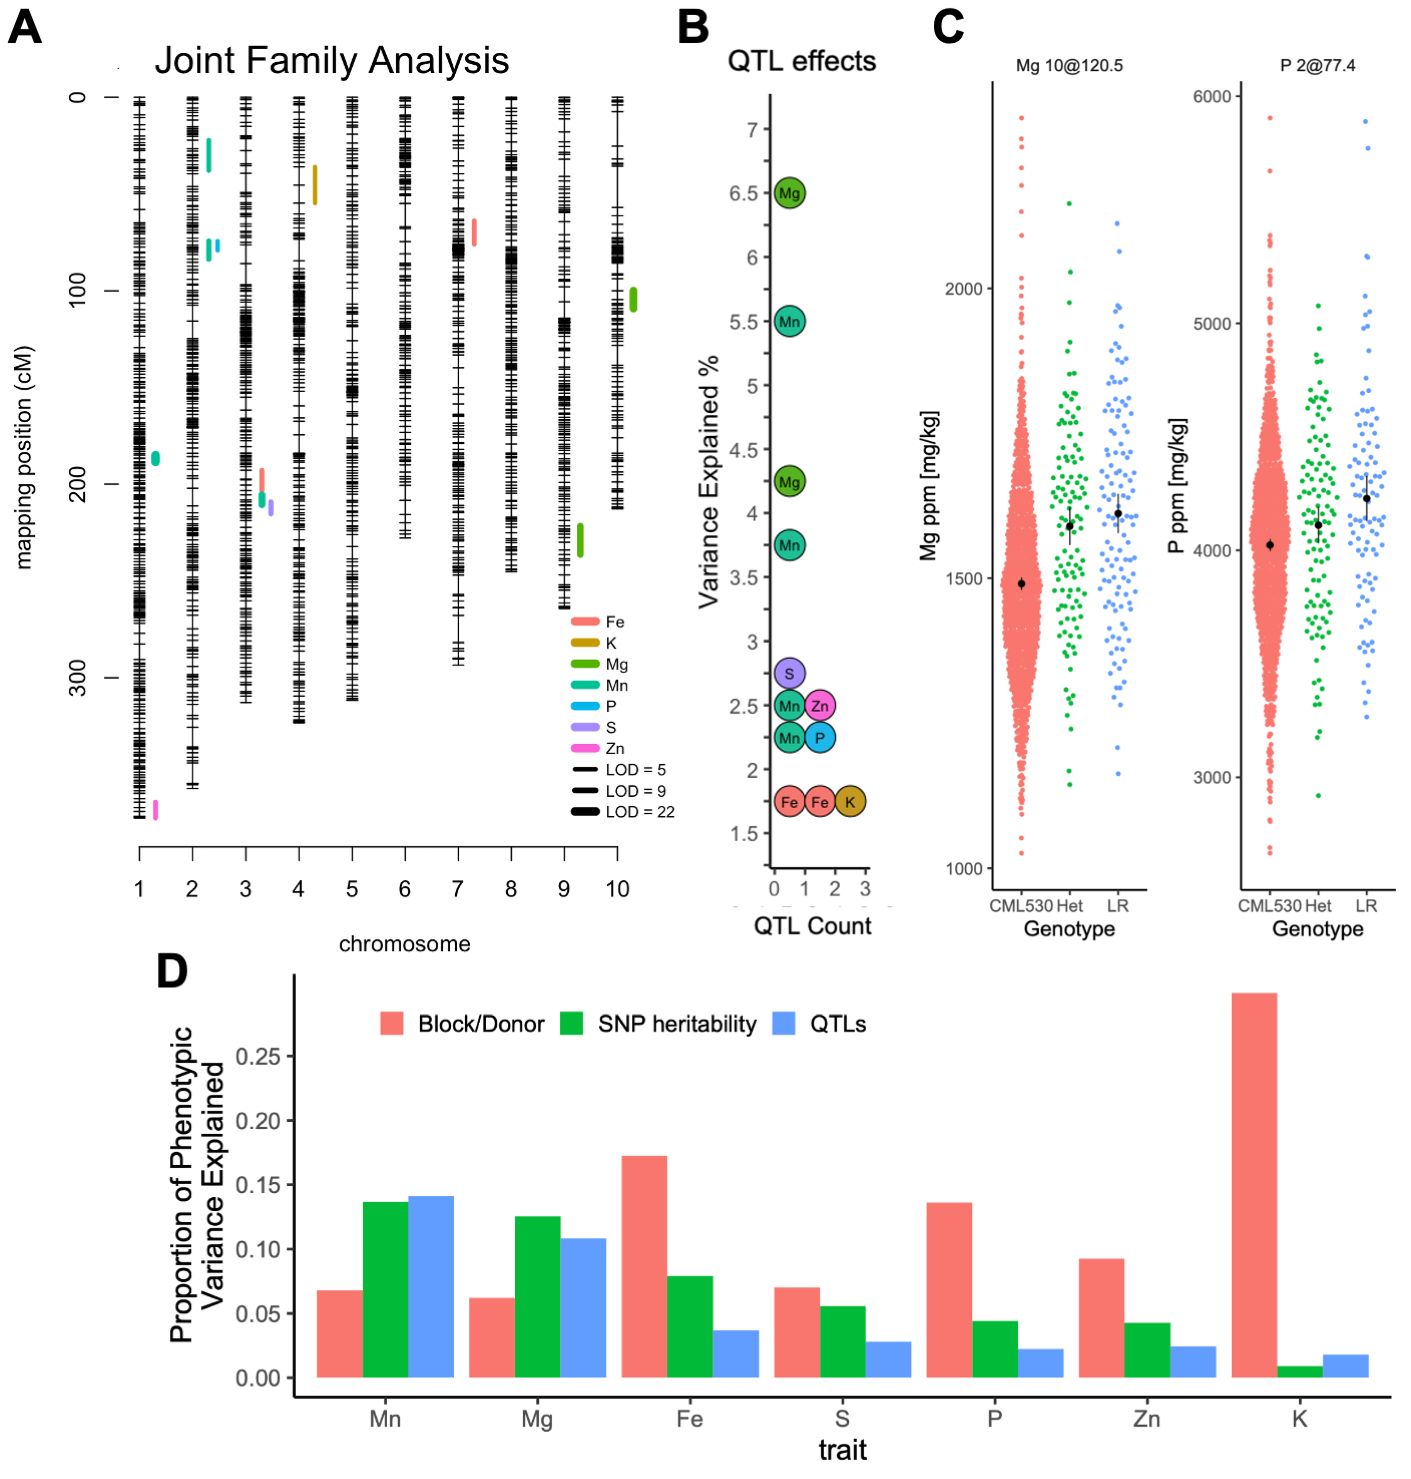
\includegraphics[width=\linewidth]{Chapter-4/figs/mineral_qtls.png}
\caption[Kernel Mineral QTLs for the AIR panel]{\textit{\textbf{Kernel Mineral QTLs for the AIR panel}}
\textbf{(A)} Significant QTLs in joint mapping analysis.
\textbf{(B)} QTL effects as percentage of observed variance in the mineral content. \textbf{(C)} QTL effect sizes, as ppm, for Mg, largest observed effect, and P
\textbf{(D)}  Phenotypic Variance Contributions. Comparison of variance contributions in separate models. Narrow sense heritability ($h^2$) estimated from variance components of a genomic relationship animal model implemented in ASReml.
}
\label{fig:mineralQTL}
\end{figure}
\clearpage

\begin{figure}[b]
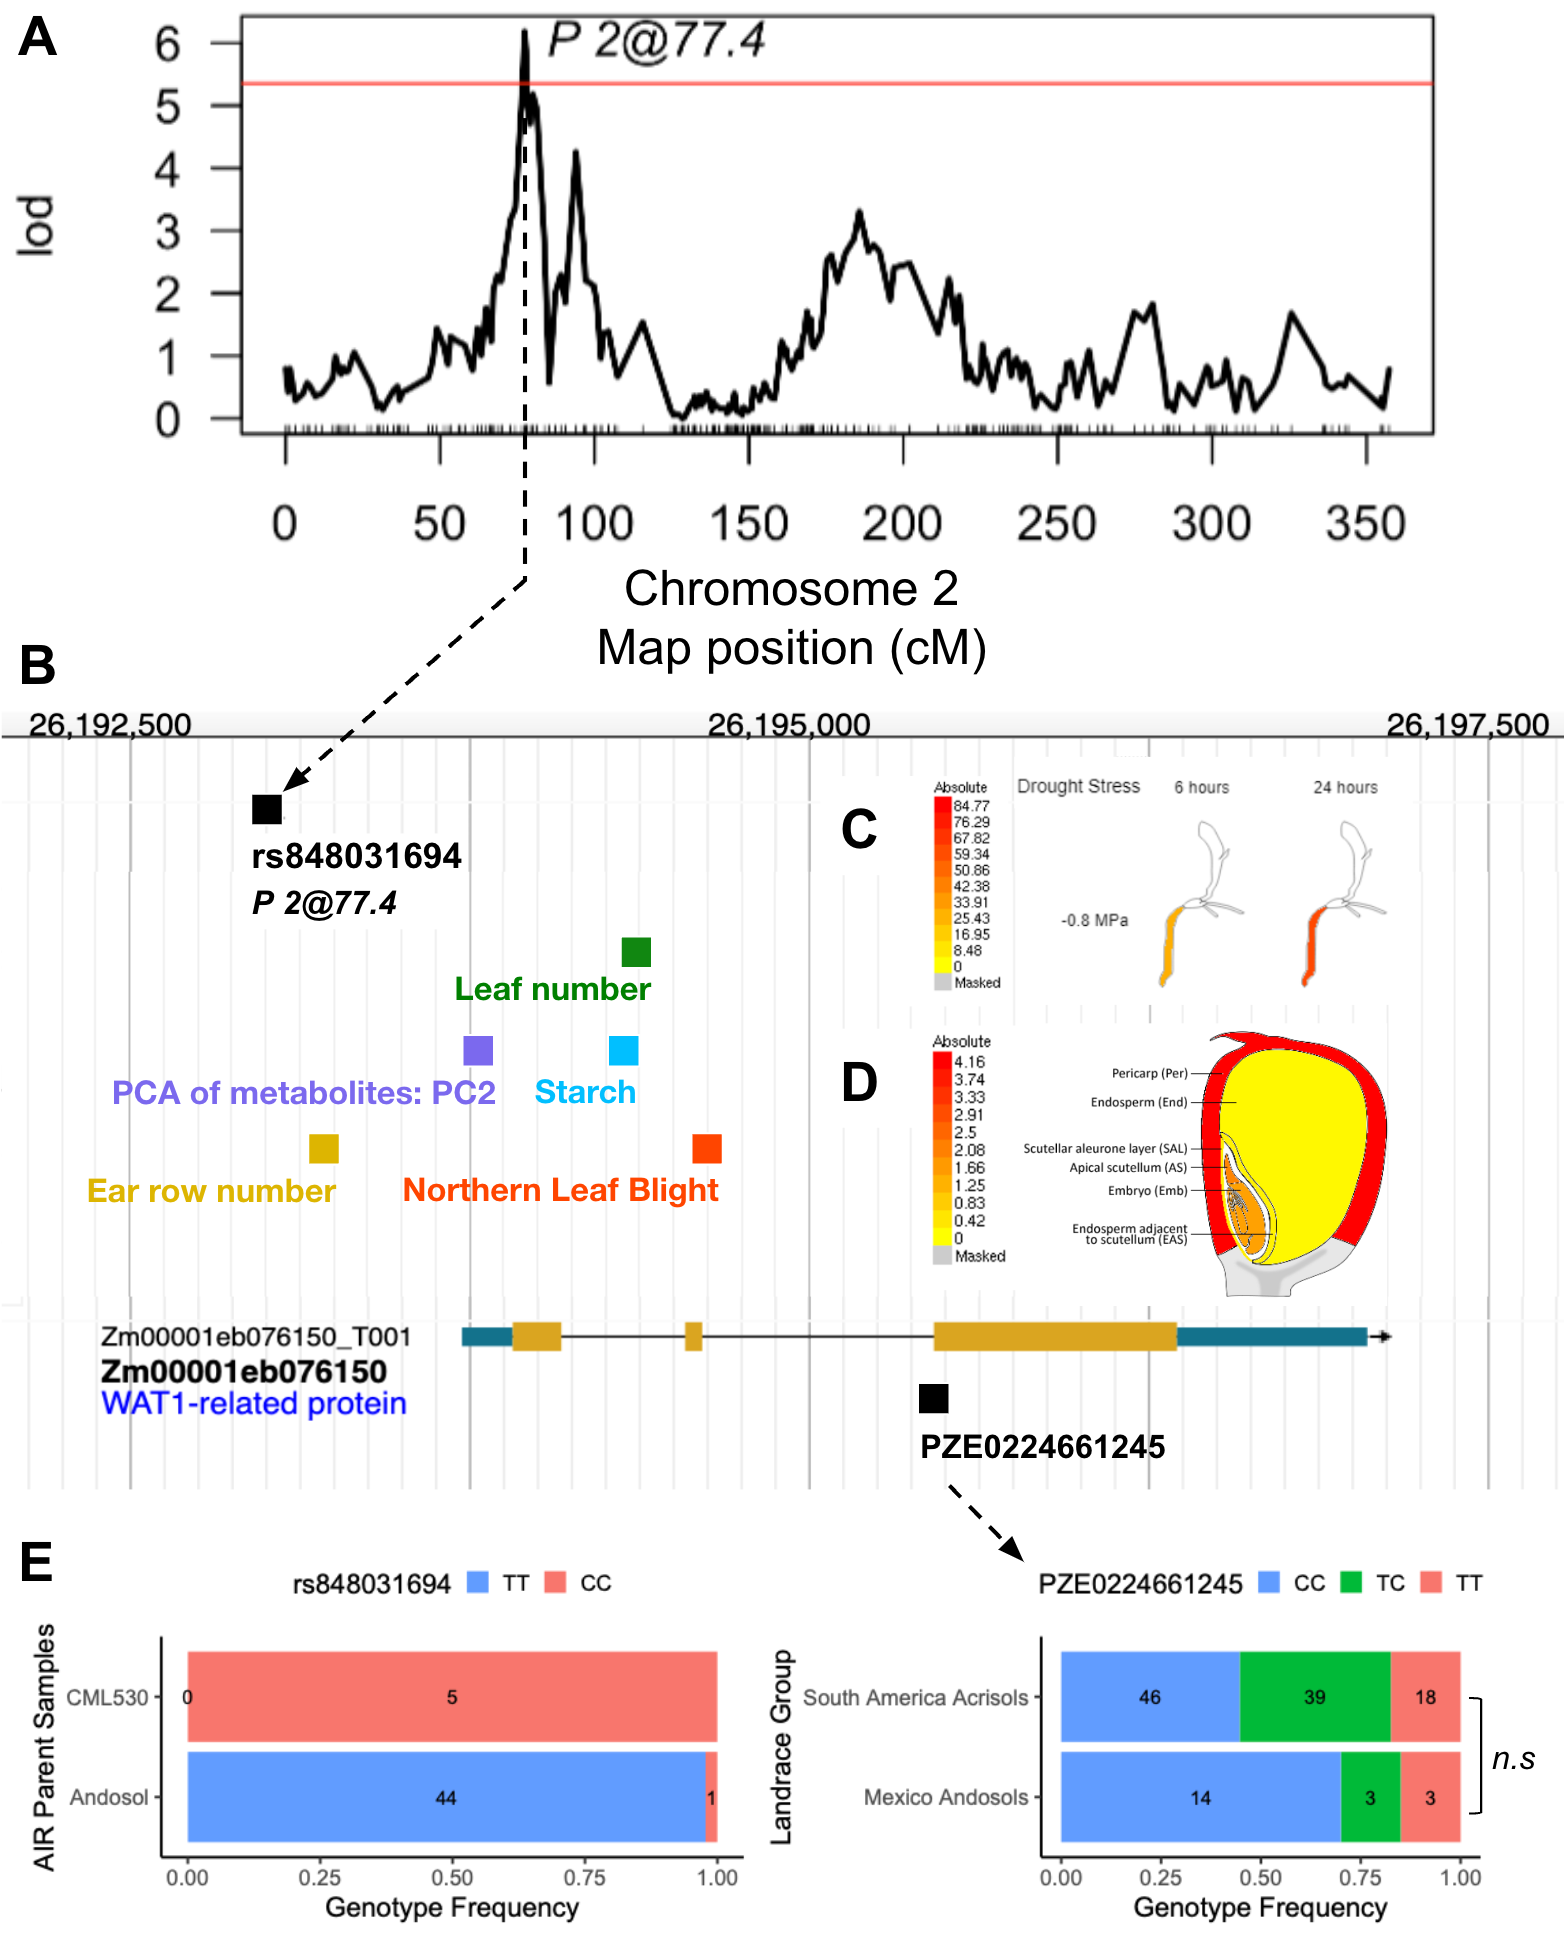
\includegraphics[width=\linewidth]{Chapter-4/figs/WAT1.png}
\caption{}
\label{fig:WAT1}
\end{figure}

\clearpage

\addtocounter{figure}{-1}
\begin{figure} [t!]
  \caption[Kernel Phosphorus QTL genomic context]{\textit{\textbf{Kernel P QTL genomic context.}} \textbf{(A)} P 2@77.4 QTL peak marker (rs848031694)
  \textbf{(B)} rs848031694 is ~1500 bp upstream of WAT1 an auxin transporter showing GWAS associations with several phenotypes under phosphorus sufficiency (colored tracks). A homolog of WAT1 in wheat has been found to be associated with root architecture under phosphorus deficiency. It is highly expressed in the pericarp \textbf{(C)} and embryonic root under drought stress \textbf{(D)}.
  %This region also shows signals of selection during maize domestication/improvement, which most likely means that some specific alleles from teosinte were recruited to cultivated maize at this site. 
  \textbf{(E)} Although there is an intronic SNP in WAT1 that has an allelic frequency higher in a sample of Mexican Andosol landraces compared with  South American Acrisols (where the recurrent parent was bred) it shows no significant evidence of selection according to soil type.}
\end{figure}

\section{Discussion}

\printbibliography[heading=subbibintoc, title=References]



%%---------------------------------------------------------------------------%%
% Appendices
%% \ensureoddstart
% uncoment lines with %% for final version
%% \restoregeometry
%% \appendix
%\newgeometry{margin=1in,lmargin=1.25in,footskip=\chapterfootskip, includehead, includefoot}

% Can remove or add
%% \chapter{Acronyms}

A summary of all acronyms is documented in Table \ref{tab:acro}.

\begin{longtable}{| l | l |}
\caption{A summary of acronyms used in alphabetical order.}\label{tab:acro}\\
\hline
Acronym & Abbreviation \\
\hline
African Easterly Wave & AEW \\
African Easterly Jet & AEJ \\
African Monsoon Multidisciplinary Analysis & AMMA \\
Climate Forecasting System Reanalysis & CFSR \\
Convective Available Potential Energy & CAPE \\
Dry Adiabatic Lapse Rate & DALR \\
European Centre for Medium Range Weather Forecasting & ECMWF \\
Eddy Kinetic Energy & EKE \\
GARP Atlantic Tropical Experiment & GATE \\
Global Forecast System & GFS \\
Global Precipitation Mission & GPM \\
Long Wave (Radiation) & LW \\
Mesoscale Convective System & MCS \\
National Aeronautical and Space Administration & NASA \\
National Center for Atmospheric Research & NCAR \\
National Center for Environmental Prediction & NCEP \\
National Hurricane Center & NHC \\
National Science Foundation & NSF \\
Planetary Boundary Layer & PBL \\
Potential Vorticity & PV \\
Short Wave (Radiation) & SW \\ 
Quasi-Geostrophic & QG \\
Rossby Wave & RW \\
Tropical Cyclone & TC \\
TRMM Multi-Satellite Precipitation Analysis & TMPA \\
Tropical Rainfall Measurement Mission & TRMM \\
Weather Research and Forecasting Model & WRF \\
\hline
\end{longtable}


% \chapter{Variables}

A summary of all variables is documented in Table \ref{tab:vars}.

\begin{longtable}{| l | l |}
\caption{A summary of common meteorological variables and their abbreviations in alphabetical order.}\label{tab:vars}\\
\hline 
Variable & Abbreviation \\
\hline
Arbitrary variable & $X$ \\
Absolute vorticity vector & $\vec{\eta}$ \\
Coriolis parameter & $f$ \\
Gas constant for dry air & $R$ \\
Geopotential & $\Phi$ \\
Geopotential height & $Z$ \\
Gravitational accelleration & $g$ \\
Horizontal wind vector & $\vec{V}$ \\
Isobaric vertical motion & $\omega$ \\
Latent heat of vaporization & $l_v$ \\
Meridional unit vector & $\hat{j}$ \\
Meridional wind & $v$ \\
Potential temperature & $\theta$ \\
Potential vorticity & $P$ \\
Pressure & $p$ \\
Relative vorticity vector & $\vec{\zeta}$  \\
Specific density & $\alpha$ \\
Specific heat capacity at constant pressure & $c_p$ \\
Temperature & $T$ \\
Time & $t$ \\
Three-dimensional wind vector & $\vec{U}$ \\
Vertical absolute vorticity & $\eta$ \\
Vertical unit vector & $\hat{k}$ \\
Vertical relative vorticity & $\zeta$ \\
Zonal unit vector & $\hat{i}$ \\
Zonal wind & $u$ \\
\hline
\end{longtable}
%% \restoregeometry

%%---------------------------------------------------------------------------%%

%%---------------------------------------------------------------------------%%
\backmatter

\end{document}